\chapter{Introduction to Stereophotogrammetry}\label{chap:stereophotogrammetry}
\section{Digital Surface Models}\commanue{Là c'est en reprendre car tu as copié collé ce paragraphe dans l'intro donc à voir comment tu équilibres entre l'intro et ici. Ici il faudra plus détailler. Dans l'intro tu te limites à expliquer brivèevemnt un DSM, la différence avec un DTM (juste le sol), les différentes méthodes possibles avec leur niveau de résolution et le niveu de détail. Ici tu peux pousser la comparaison, tu peux montrer les différentes produits. Peut-être ici donner des exemples montrer une ville, genre toulouse,  avec différents DSM pour voir les différents niveaux de détails, parler des formats etc. Tu peux aussi parler de l'étendue spatiale des produits, de leur mise à jour. Pour l'instant pas mal d'interventions manuelles.}
\todoroman{Utiliser les slides de formation CARS pour montrer les différentes méthodes pour faire de la 3D, mettre des exmples de LiDAR ou faire un schéma ?}

\commanue{Il faudrait aussi montrer des résultats, en gros c'est quoi en fait un modèle 3D. Après parmi tous les exemples d'utilisation de la 3D que tu donnes tu peux en détailler un un peu plus. Celui que tu préfères.}
Knowing the Earth's topography is crucial for modern geosciences. As such, \acrfull{dsm}, which are a representation of a surface's elevation on a regular grid, appear as a natural solution in many \acrfull{gis}. Indeed, they can easily be handled and provide georeferenced information regarding the topography of an area. \acrshort{dsm} find usage in various contexts for a wide range of applications. In \acrfull{eo} for instance, \acrshort{dsm} are used to monitor changes in vegetation \cite{sadeghi_canopy_2016}, melting rates of glaciers \cite{berthier_glacier_2014, rieg_pleiades_2018}, volcanos \cite{ganci_data_2022}, snow or water resources \cite{marti_mapping_2016, gascoin_theia_2019, yamazaki_merit_2019} \etc Similarly, \acrshort{dsm} are employed for catastrophe management, to predict the potential damage caused by earthquakes or floods \cite{jenkins_physics-based_2023} \dots \acrshort{dsm} are also crucial for ortho-rectifying image, \ie geometrically correcting the effects of distortions between the sensor and the terrain. This process creates a planimetric image with a consistent scale in all parts of the image. It allows images to be easily used in \acrshort{gis} or as background for maps. In urban settings, high resolution \acrshort{dsm} can help drone navigation for Defense applications, or more broadly for urban planning \cite{velazco_3d_2012}.

Nowadays, \acrshort{dsm} are mostly generated from laser scanning with LiDAR sensors, radar interferometry or stereophotogrammetry \cite{youssefi_cars_2020}. Air-borne laser scanning results in \acrfull{vhr} models, but the swath width and cost of acquisition campaigns do not allow to periodically cover the globe\commanue{Pour le LIDAR tu peux citer le Liadr HD de l'IGN: durée de la campagne et données déjà disponible pour montrer que rien que pour avoir la France cela prend beaucoup de temps.}. Space-borne \acrshort{lidar} is mostly used for atmospheric measurements, or discrete measurements \cite{fouladinejad_history_2019}. For instance, NASA's ICESat-2 \cite{jasinski_atlasicesat-2_2020} measures elevation of seas and glaciers using 6 lasers taking measurements along track, which is not adapted for reconstructing high-accuracy DSM. Space-borne radar interferometry remains widely used, and has allowed to create a worldwide digital model of emerged surfaces of the Earth at $30$m and $90$m resolution with the SRTM mission \cite{farr_shuttle_2007}\commanue{Tu peux aussi citer le DEM Copernicus https://spacedata.copernicus.eu/collections/copernicus-digital-elevation-model il faudrait détailler comment il est réalisé. Le SRTM c'est la classe car c'est via la navette Endeavour. Pour revenir au DEM copernicus, il est réalisé à partir de Tandem-X qui est un SAR qui permet de réaliser des DEM jusqu'à 10 à 12m. En fonction du temps tu peux détailler un peu le principe d'acquisitions}. To obtain coarser resolutions\commanue{Donne des ordres de grandeurs qu'on vise par rapport aux autres technos}, it is possible to leverage the technological advancement of optical sensors in orbit to create sub-meter \acrshort{dsm} using stereophotogrammetry with relatively low cost\commanue{Peut-être détailler pourquoi c'est plus low cost}. However, this process is more complex than laser measurements as it deduces height from the principle of parallax. Stereophotogrammetry pipelines usually consists in multiple processing steps with intermediary products (see \ref{sec:classical_stero_pipeline}), with different methods, parameterization and post-processes available for each step (\eg matching, filtering \etc). This broad range of solutions allow to adapt our processes to the type of images and terrain observed, but it sometimes makes it difficult to determine the configuration producing the best quality DSM, or to single out a general good-working configuration. 

This thesis focuses on \acrshort{dsm} obtained from stereophotogrammetry, however we will use \acrshort{dsm} obtained from air-borne LiDAR acquisitions as references to validate our results, considering their high resolutions\commanue{Dans cette section tu mentionnes rapidement le lidar. Je pense que tu dois détailler un peu plus car c'est comme même ta vérité terrain. Il faadrait parler de l'acquisition, du format (points), de la rasterisation (on se retrouve avec plusieurs bandes). Il faudrait aussi citer le lidarHD de l'IGN car c'est vraiment cela que tu utilises comme VT. Tu peux mettre en perspective le temps nécessaire pour faire les acquisitions et mettre à dispo les produits. Notamment cela te sera utile quand tu aborderas la mission CO3D}.
\commanu{ pas plus que manue sur cette section, complètement d'accord}
\todoroman{Schema de \acrshort{dsm} par avion LiDAR, satellite interfero et stereo}
\section{CO3D mission and Pléiades Satellites}\label{sec:co3d}\commanue{Moi je mettrais un titre plus générique sur les satellites optiques haute résolution. Tu démarres par DSM dans la section précédente et tu mentionnes ce type de satellites pour créer des DSM. Donc section suivantes tu parles de ces satellites que l'on peut utiliser pour faire de la 3D (ah transition !) car ils possèdent des atouts : haute résolution, agilité. Tu peux mentionner ensuite les satellites existants Worldview Pleiades CSO (acquisition push-broom que tu peux introduire si tu veux) et ensuite tu introduis la nouvelle constellation de satellites CO3D matrice de bayer, ils volent en formation donc acquistion synchrone (pour une paire),etc. Te connaissant je ferais des sous-sections par exemple : intro globale sur les sat optiques HR, mission actuelles, mission CO3D, données que tu utilises}\commanu{+1}

The following paragraphs detail satellites characteristics relevant to stereophotogrammetry. It is important to notice that although the sensor used greatly determines the resolution of the final \acrshort{dsm}, it is not the only factor at stake here. The altitude and positions of the satellites are also crucial for the resolution\todoroman{parler de \cite{qin_critical_2019} avec un bon ratio et surtout la diff d'angles solaires}, and can be characterized by the \acrfull{b/h} ratio, as in \Cref{fig:RPC}. This ratio is computed by dividing the distance separating the stereo acquisitions by the altitude of the satellite. It indicates the angle formed between the line of sights originating from the satellites towards an object of the scene. A high \acrshort{b/h} allows for high elevation accuracy, but possesses more occluded regions (for instance a narrow street between two high buildings), and conversely for a low B/H \cite{delon_small_2007}.

The main source of images used in this thesis comes from Pléiades images\commanue{Tu peux mentionner çà à la fin de la section (tu sais le truc qui s'appelle une conclusion) une fois que tu as présenter les différentes mission et leur caractéristiques. Tu peux dire que bien que les travaux de cette thèse ont pour vocation de servir dans le segment-sol de CO3D en l'absence de donnée CO3D tu as utilisé des données Pléiades qui ont caractérisques assez proches.}. The Pléiades constellation developed by Airbus is composed of two identical satellites, 1A and 1B. The satellites were launched in 2011 and 2012 in an heliosynchronous orbit at $690$km, for both civilian and defense usages. They provide panchromatic images at a resolution of $70$cm (resampled at $50$cm), and RGB-NIR images at a resolution of $2$m, with a $20$km swath (\url{https://dinamis.data-terra.org/pleiades/}). Their high agility and revisit rate allow them to capture stereo and tri-stereo images for any location on the globe, ideal to produce \acrshort{dsm} with high accuracy\commanue{Il y a même un mode vidéo où tu prends plus d'une dizaine images}. The \acrshort{b/h} ratio for stereo acquisitions can vary between $0.1$ and $0.4$. However, stereo acquisitions is not the only objective of this mission, even though the demand for those products is increasing \cite{berthier_glacier_2014, poli_radiometric_2015, rieg_pleiades_2018, loghin_potential_2020}. The acquisition of stereo images is thus provided on command, which can conflict with other usages of the satellite, and can become costly when trying to cover large areas \commanue{Tu peux mentionner que c'est un satellite dual donc militaire et civil et que les militaires ont la priorité. Après tu peux aussi dire que Pléiades est utilisé lors de l'activation de la chartre https://disasterscharter.org/fr/web/guest/home. Alors on a pas déclenché la chartre mais pour le glissment de terrain dans le sud-est Pléiades avait pris de stéréo.}.  
\begin{figure}
    \centering
    \begin{subfigure}[t]{0.5\linewidth}
        \centering
        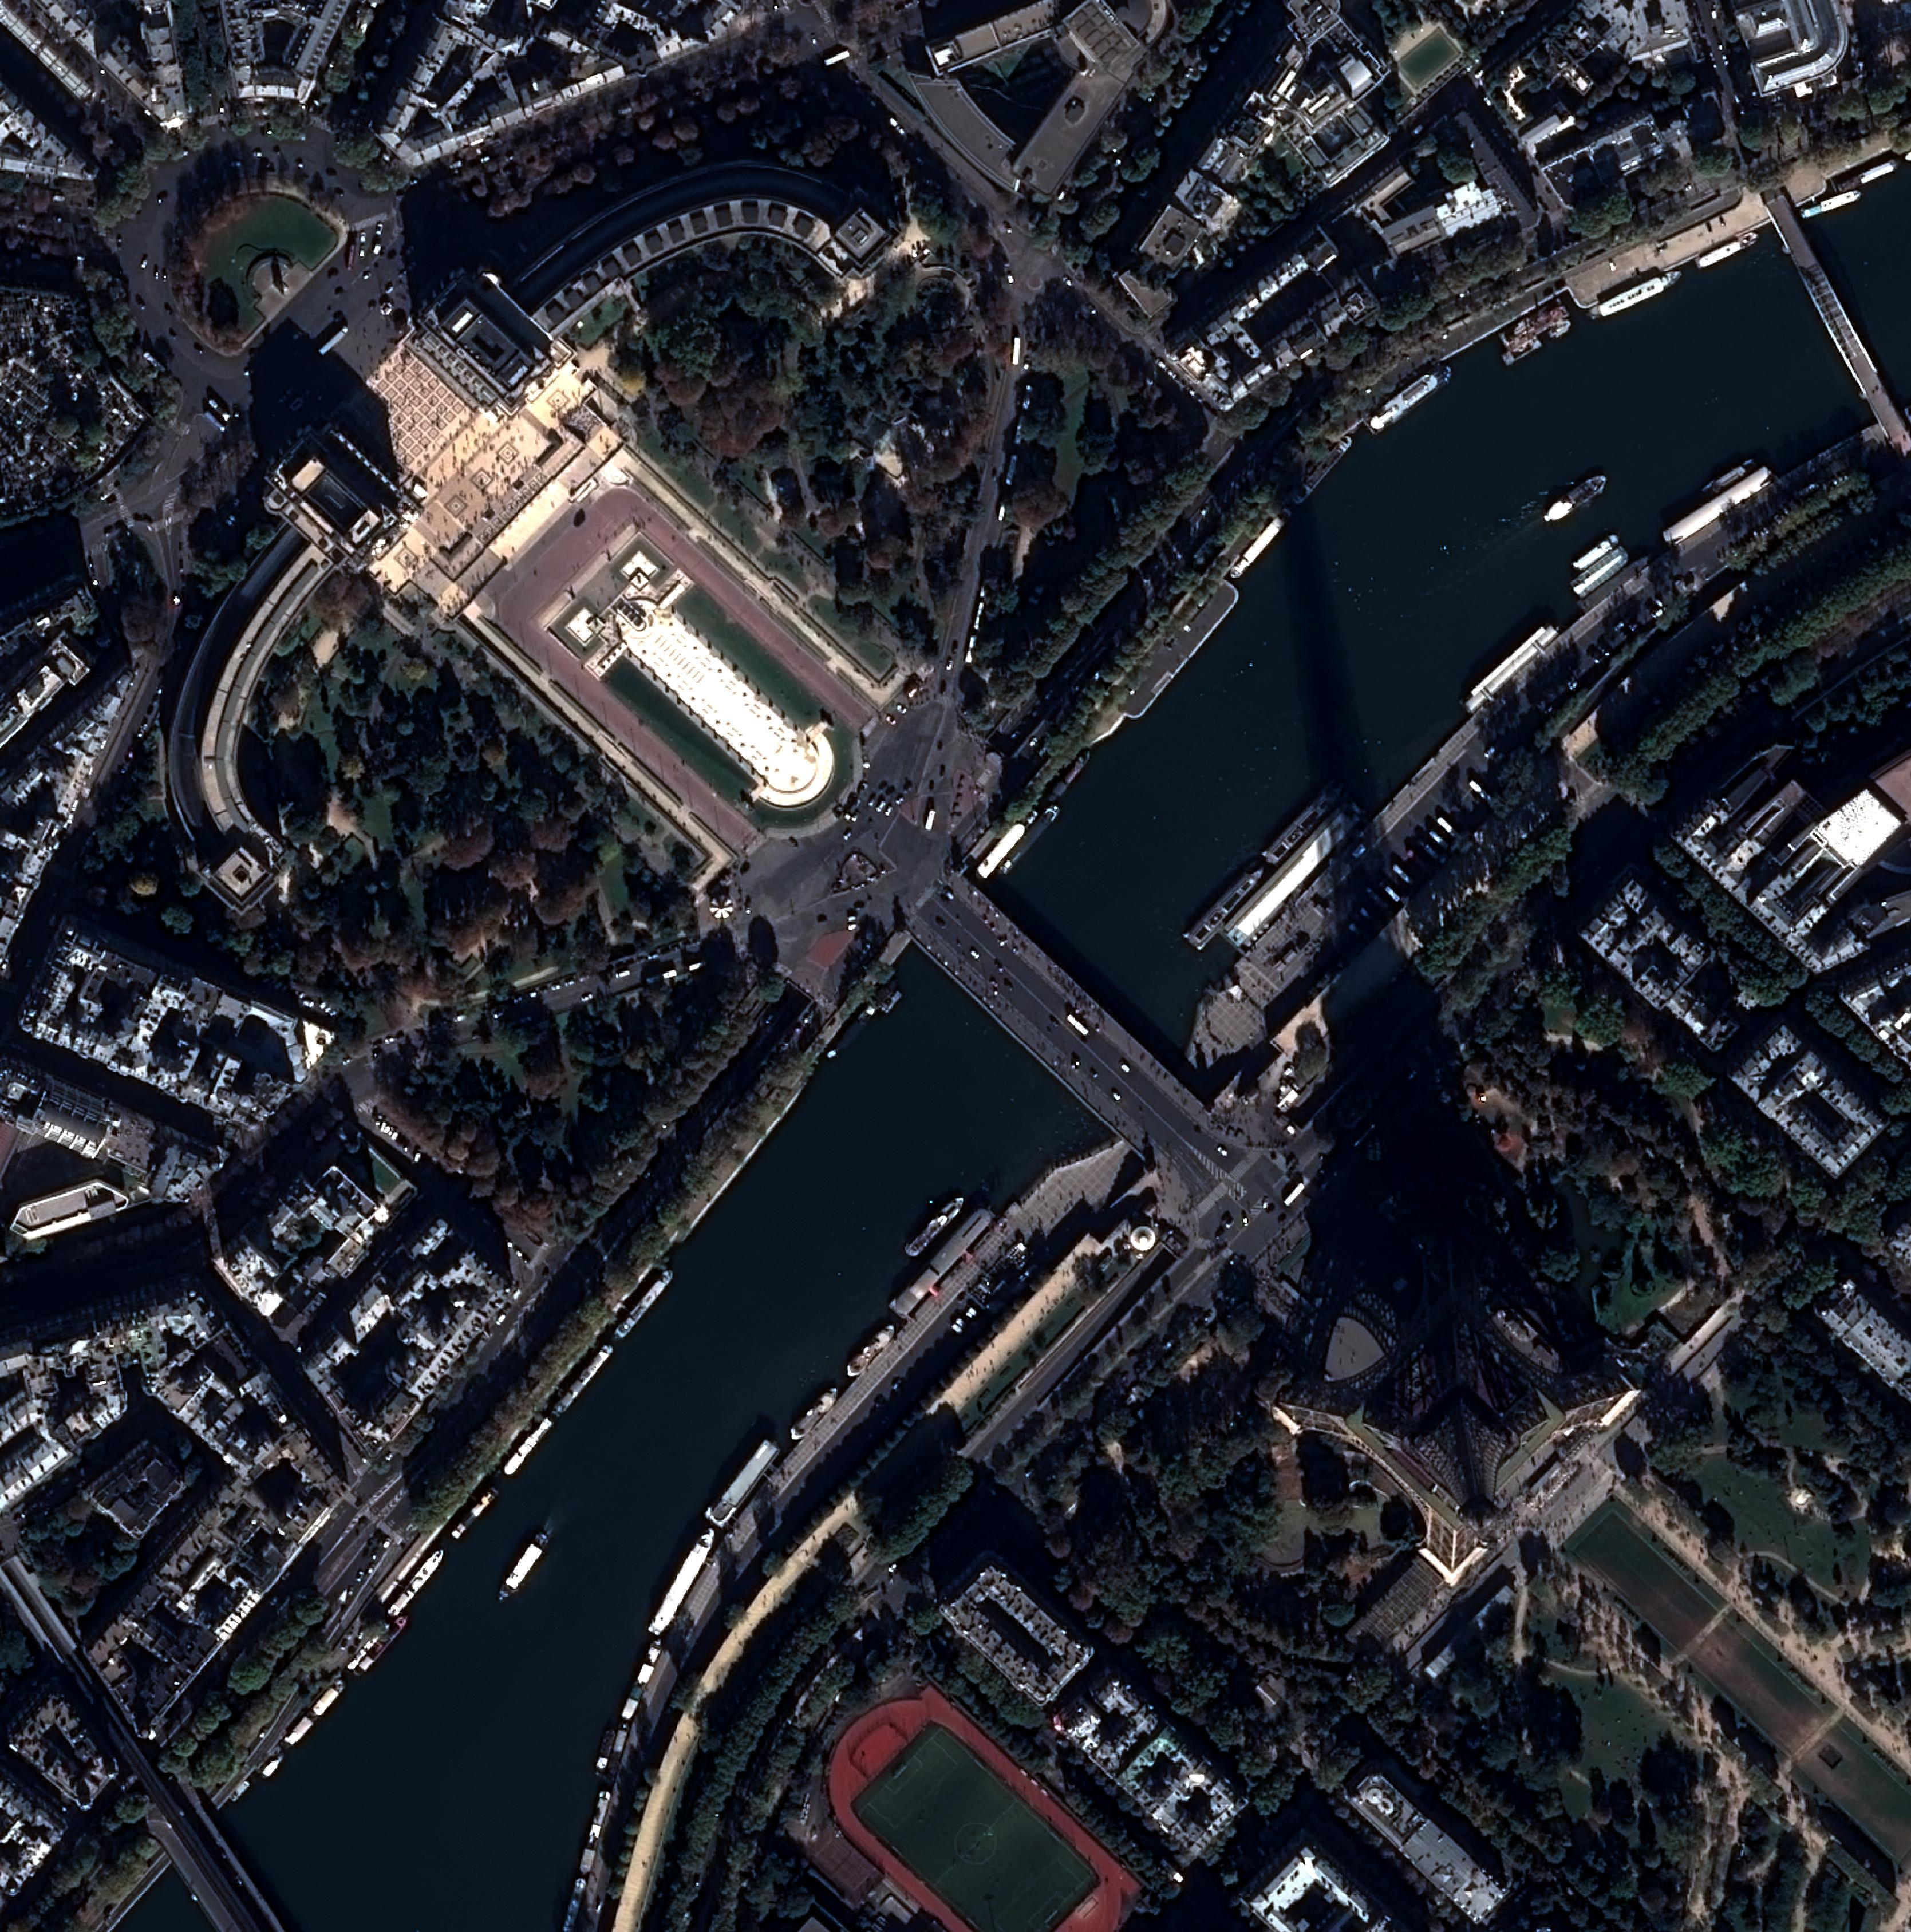
\includegraphics[height=6cm]{Images/Chap_1/Paris_003.jpeg}
        \caption{$14/10/2017$ $11:03:003$}
        \label{fig:Pleiade_over_Paris_a}
    \end{subfigure}\hfill
    \begin{subfigure}[t]{0.5\linewidth}
        \centering
        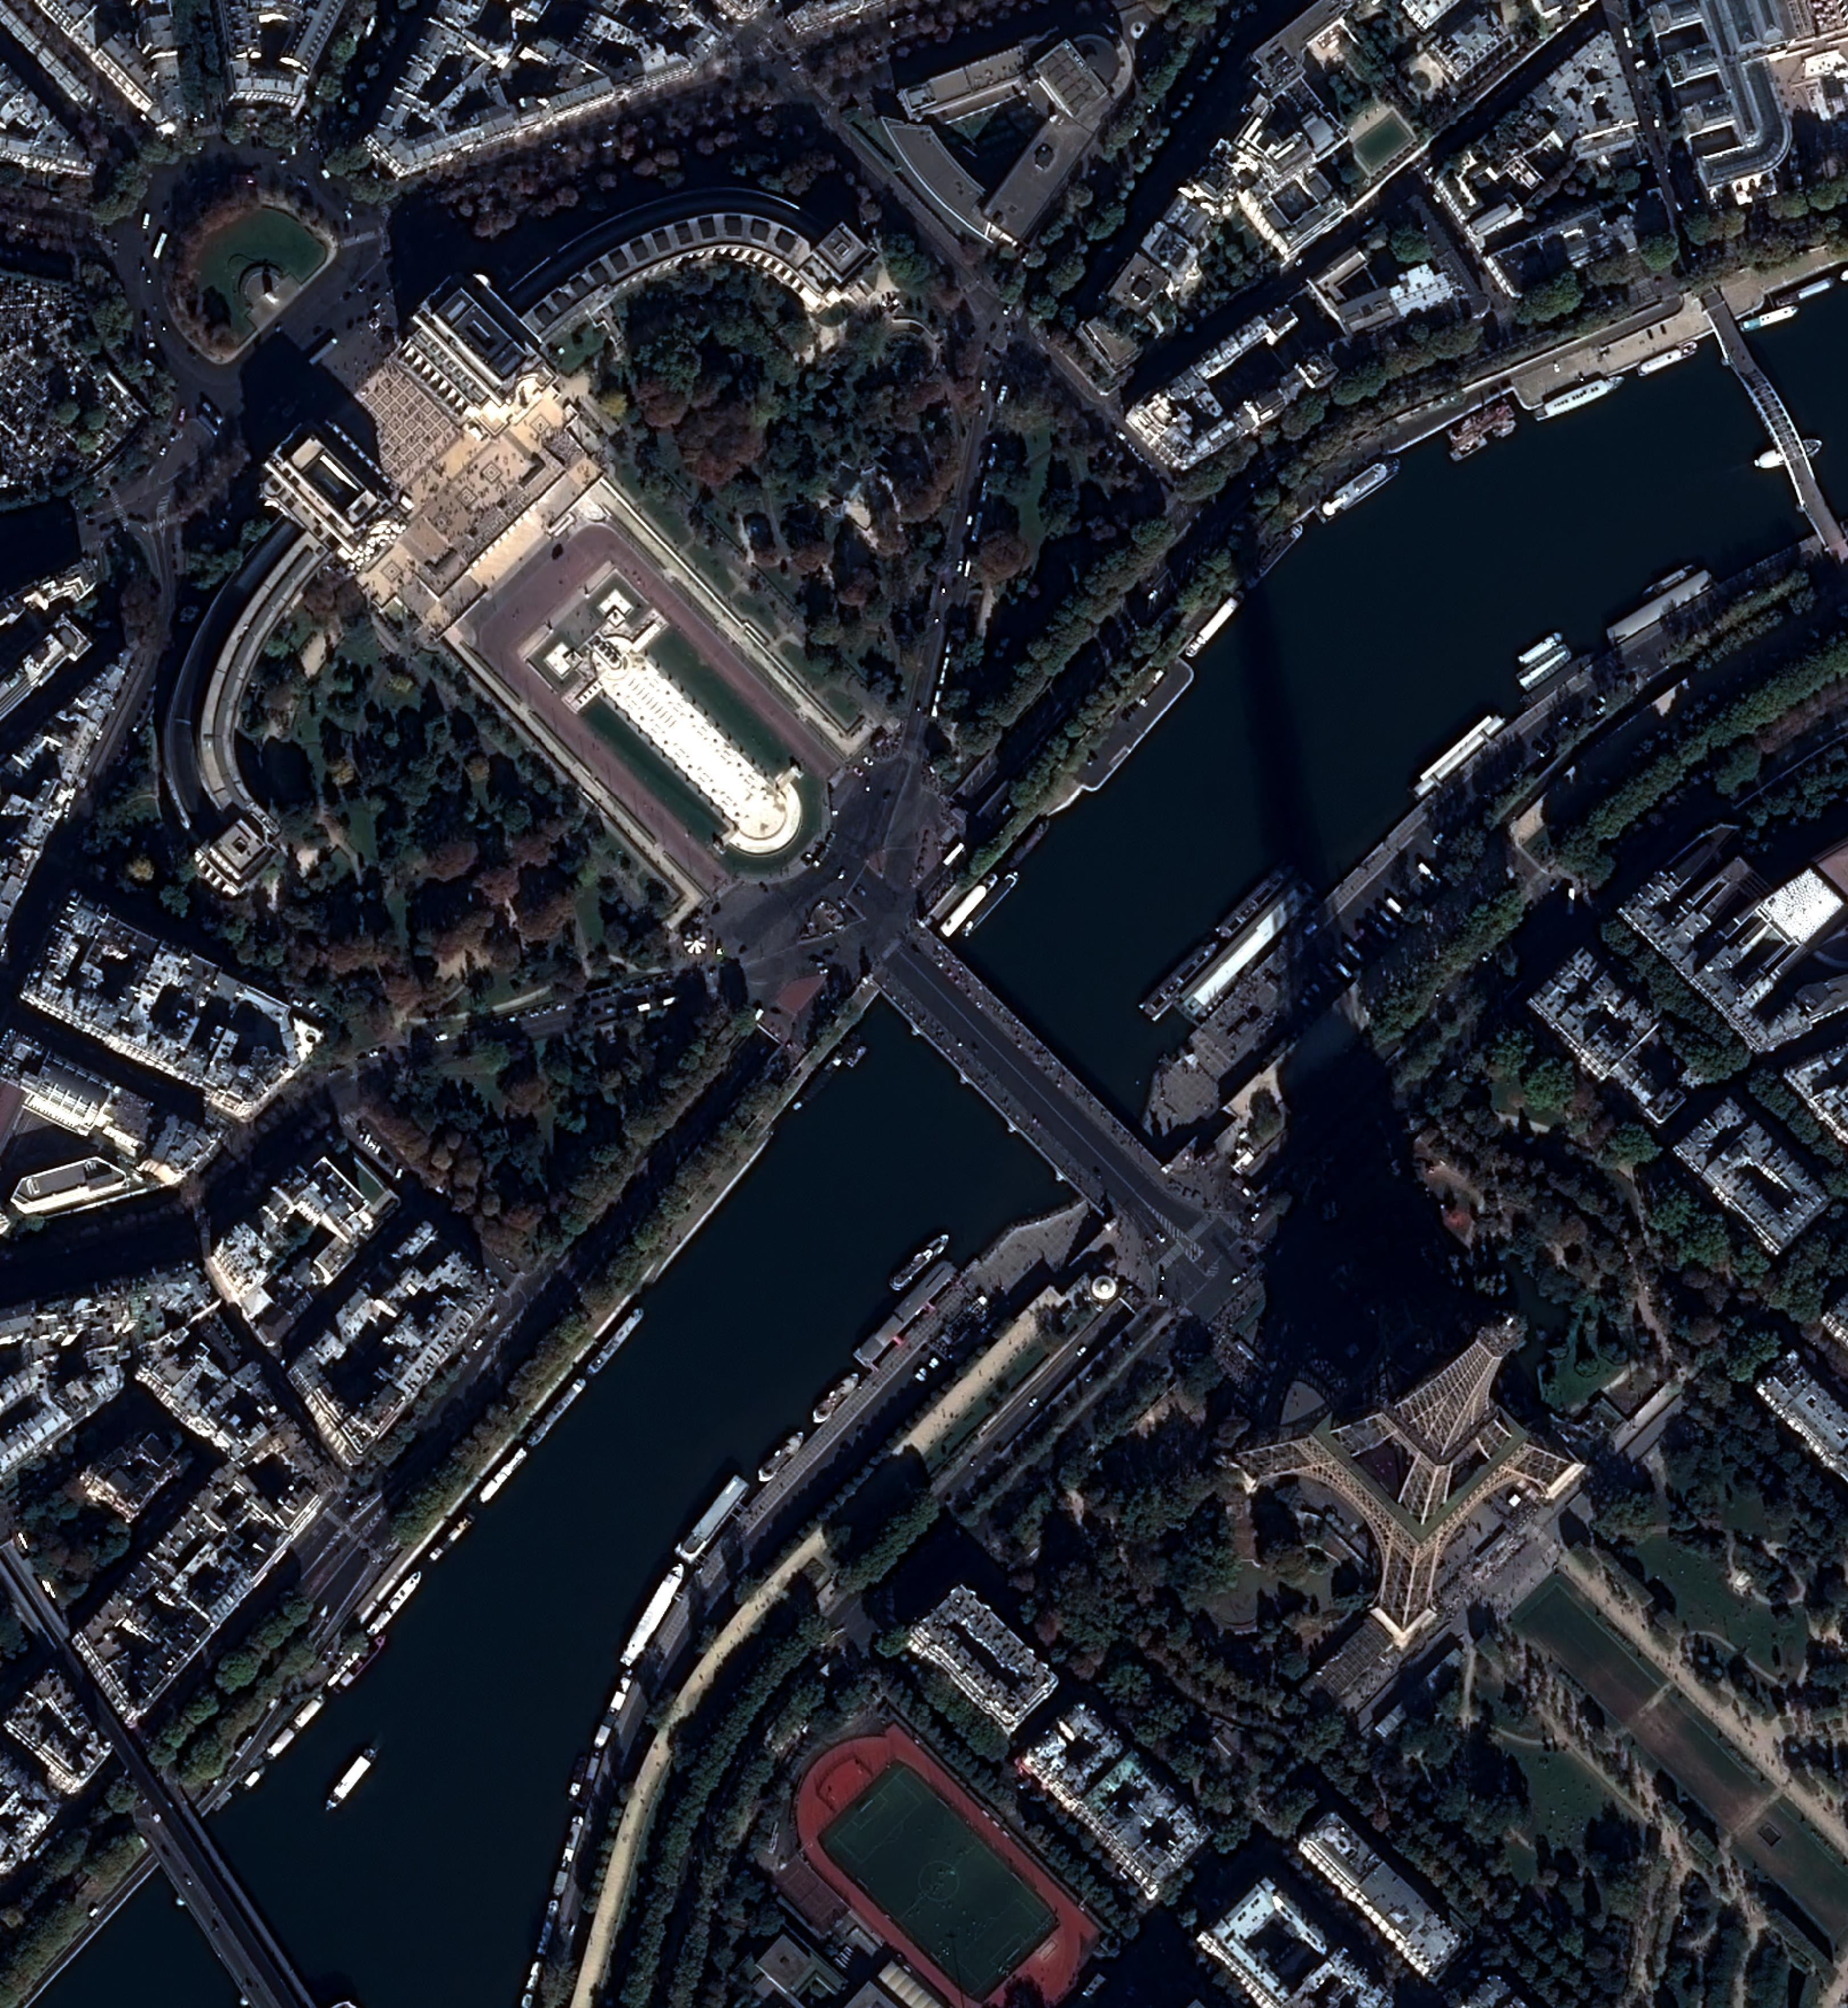
\includegraphics[height=6cm]{Images/Chap_1/Paris_403.jpeg}
        \caption{$14/10/2017$ $11:03:403$}
        \label{fig:Pleiade_over_Paris_b}
    \end{subfigure}
    \caption{Pansharpened Pléiades stereo images over Paris at $0.5$m of resolution. Pléiades \copyright CNES 2017, Distribution AIRBUS DS}
    \label{fig:Pleiade_over_Paris}
\end{figure}

In order to produce a worldwide \acrshort{dsm} with $1$m resolution by 2025, the \acrfull{cnes} is launching the \acrfull{co3d} mission \cite{melet_co3d_2020}. Composed of two pairs of low-cost satellites equipped with \acrshort{vhr} optical sensors, the mission will produce image in the \acrshort{rgb} and \acrshort{nir} spectrum at $0.5$m of resolution \cite{lebegue_co3d_2020}. The pairing of satellites allows for \textit{almost} simultaneous stereo image acquisition, cutting short the transient object problem (\ie objects moving/disappearing between stereo images). To be able to process the amount of data provided by the CO3D mission ($40\,000$ images a day, at $50cm$ resolution and covering a footprint of $7km\times5km$ \cite{melet_co3d_2020, lebegue_co3d_2020}), every step of the pipeline has been developed to be highly parallelizable\commanu{scalable ? to be scalable -> passer à l'échelle. plus large que juste le calcul parallèle qui est une facette de l'optim}. Different acquisition schemes can also be used, such as the video mode, or even the `diamond' geometry acquisition, which acquires a quadri-stereo over a couple of days. Depending on the relief of the terrain observed, the \acrshort{b/h} ratio will be between $0.2$ and $0.3$\commanue{Détaille un peu dans les paysages naturels, les satellites s'éloignent pour augmenter le B/H et dans les zones urbaines ils se rapprochent pour limiter les occlusions}. In parallel with image quality specifications, the CO3D products need to abide to a height accuracy of $1$m on low slopes \comloic{à vérifier je crois que c'est 1m en relatif à CE90. En absolu je ne sais plus}. Another requirement, which is particularly relevant in the context of this thesis, is the production of a performance map supporting the output \acrshort{dsm}. Investigating sources and propagation of the uncertainty inside a 3D stereo pipeline can be beneficial for this performance map requirement\commanue{Je dirais plutôt In addition, the project plans to produce a performance map supporting the output DSM. Therefore, investigating sources and propagation of the uncertainty inside a 3D stereo pipeline is essential for the implementation of this performance map.}\commanu{idem que manue avec juste investigating uncertainty inside a 3D stereo... serait plus direct, tu parles des sources et propagation ailleurs, pas besoin de compliquer la phrase}. 
\todoroman{Dire qu'on est partis du besoin utilisateur pour faire notre méthode et pas l'inverse.}\commanue{Effectivement tu peux expliquer que pour répondre à ce besoin de créer une carte de performance, il existe plusieusr approches. On pourrait faire comme ce qui est fait dans les autres produits (attention c'est à vérifier sur les sites de l'IGN et du DEM coppernicus par ex) il y a une carte qui indiquent une classe de confiance dans le résultat. C'est souvent un masque avec des flags de qualité qui permet de dire si le traitement c'est bien passé ou non. Toi tu as choisi une optique différente en demandant aux utilisateurs quelle information d'incertitude ils attendaient. Et ensuite blabla tu connais l'histoire comme moi.}\commanu{+1}
\todoroman{Parler de Maxar avec les Worldview ?}\commanu{tu peux juste citer mais pas obligé, tu t'en sers pas...}

\todoroman{Schema de la mission CO3D. Type of sensor, push-broom vs raster for CO3D. Pour info c'est une matrice de Bayer}

\begin{remark}
    When an image is acquired both in panchromatic and RGB mode, it is possible to leverage the high resolution of the panchromatic image to improve that of the color image. This fusion technique is called \textit{pansharpening} \cite{loncan_hyperspectral_2015}. We use this technique for clarity in figures and other illustrations of this thesis. It is important to remember that the processed images are the panchromatic images, and not the pansharpened ones which are only used for the final visualization.\commanue{Pour CO3D c'est un peu différent car matrice de Bayer.}
\end{remark} 
\commanu{je sais pas si besoin de cette remarque panchro RGB ici, peut etre quand tu l'utilises plus tard ?, tu verras à la relecture finale. et oui attention différent sur CO3D}

\section{Sensors and Geolocation}\label{sec:sensors_rpc}\commanue{là la transition avec cette partie est plus complexe. Peut-être que je mettrais les éléménts concernant les différents capteurs dans le paragraphe précédent lorsque tu présentes les satellites. Et je déplacerais la partie géoloc dans le pipeline par ex dans une section au début (que tu n'as pas qui explique le niveau de produit que l'on utilise pour faire de la 3D donc image en géométrie capteur avec un modèle de prise de vue où tu peux expliquer que dans ton cas c'est un RPC car le comprimis entre précision et facilité d'utilisation est acceptable.)}
Different types of sensors can be used to acquire satellite images. Below is detailed a (non-exhaustive) list of sensors of interest \cite{cnes_imagerie_2008}

\textbf{CCD matrix sensor}. CDD are classical sensors used, for instance, in current digital cameras. They possess multiple advantages, such as good geometrical quality as all pixels are acquired simultaneously, or the possibility to perform many acquisitions with various angles possible. However, CCD sensors with small pixel sizes are technologically difficult to built. Augmenting the number of pixels complicates the shutter function\commanue{et ça prend de la place. Alors que qq lignes pour un push-broom c'est plus compact}, and requires more radiometric calibration as one pixel equals one sensor\commanue{là je ne suis pas sure de comprendre la remarque}. It is also more complex to acquire long segments of an image \commanue{il faut peut-être expliqué que le satllite est toujours en mouvement donc là tu dois faire en sorte de ralentir (façon de parler car en réalité le satellite qui pivote pour fixer la zone à aquérir suffisamment longtemps pour avoir assez de petits photons)}. CO3D satellites will use this technology\commanue{moi je mettrais cela dans la description de CO3D}.

\textbf{Push-broom sensor}. Those image sensors are only composed of a single cell row, acquiring simultaneously radiometric information alongside a line perpendicular to the direction of the satellite\commanue{peut-être précise que dans ce cas on utilise la vitesse de défilement du satellite}. As only one line of cells is needed, push-broom sensors are simple systems which can capture images continuously, while guarantying good geometrical quality along the rows of the images. A variation of those sensors are TDI sensors (Time Delay Integration). Those sensors function as a push-broom except that each row has the ability to transfer its photon charges to the next row. This allows to capture signals over a longer period of time,  thus reducing the signal-to-noise ratio. Harder to produce, TDI sensors also require a precise control of the satellite so that observed objects stay within a column of the TDI sensor. They are used in Pléiades satellites for instance\commanue{je remonterais cette partie quand tu décris les capteurs HR actuellement en vol.}.

\todoroman{Regarder "Developement and Implementation of Rational Polynomial Coefficient Algorithms for Georeferencing Cartosat-1 Data", et "Metric Information Extraction from Spot Images and the Role of Polynomial Mapping Functions" de Baltsavias et Stallmann}
\commanue{Comme mentionner précédement je mettrais cela plus loin quand tu décris le pipeline CARS. Je ferais une section dédiée sur le fait que CARS prend en entrée une image en géométrie capteur avec un modèle de prise de vue. Si tu veux tu peux préciser qu'il s'agit d'une image où les bandes sont recalées entre elles. Tu peux expliquer à quoi correspond un pixel. On est pas sur une image géoréférence comme on pourrait utiliser dans un SIG. Et ensuite c'est parti pour le modèle de prise de vue... }\commanu{d'accord avec ca}A crucial part of satellite imagery is the ability to perform georeferencement, or georegistratation, of every pixel, \ie, locate their coordinates in an Earth system of coordinates such as latitude and longitude. Physical models possess high geolocation accuracy, but are sensor-specific and are computationally complex. For stereo reconstruction,  generalized sensor models are preferred. Specifically, we will focus on \acrfull{rpc} \cite{grodecki_ikonos_2001} used by the \acrshort{co3d} and Pléiades satellites, and provided alongside images. Sometimes called Polynomial Mapping Functions \cite{baltsavias_metric_1992} or Rational Function Models \cite{tao_comprehensive_2001}, \acrshort{rpc} are functions allowing to transform a pixel's ground location $(X,Y,Z)$ into its image coordinates $(row, col)$. \acrshort{rpc} encode lines of sight of the satellite, \ie the line joining the center of the sensor's cell to the ground and going through the optical center of the sensor. To improve numerical stability and minimize computation errors, the image coordinates and ground coordinates are normalized between $-1$ and $1$, using their scale factors $SF$ and mean values:
\begin{eqnarray*}
    SF_X &=& \max(X_\mathrm{max}-\overline{X},~\overline{X}-X_\mathrm{min})\\
    \Tilde{X}&=&\frac{X-\overline{X}}{SF_X}
\end{eqnarray*}
The same processed is applied to $Y,Z,row$ and $col$. To avoid heavy notation in this section, we will refer to every normalized coordinate using their non-normalized symbol.

\begin{figure}
    \centering
    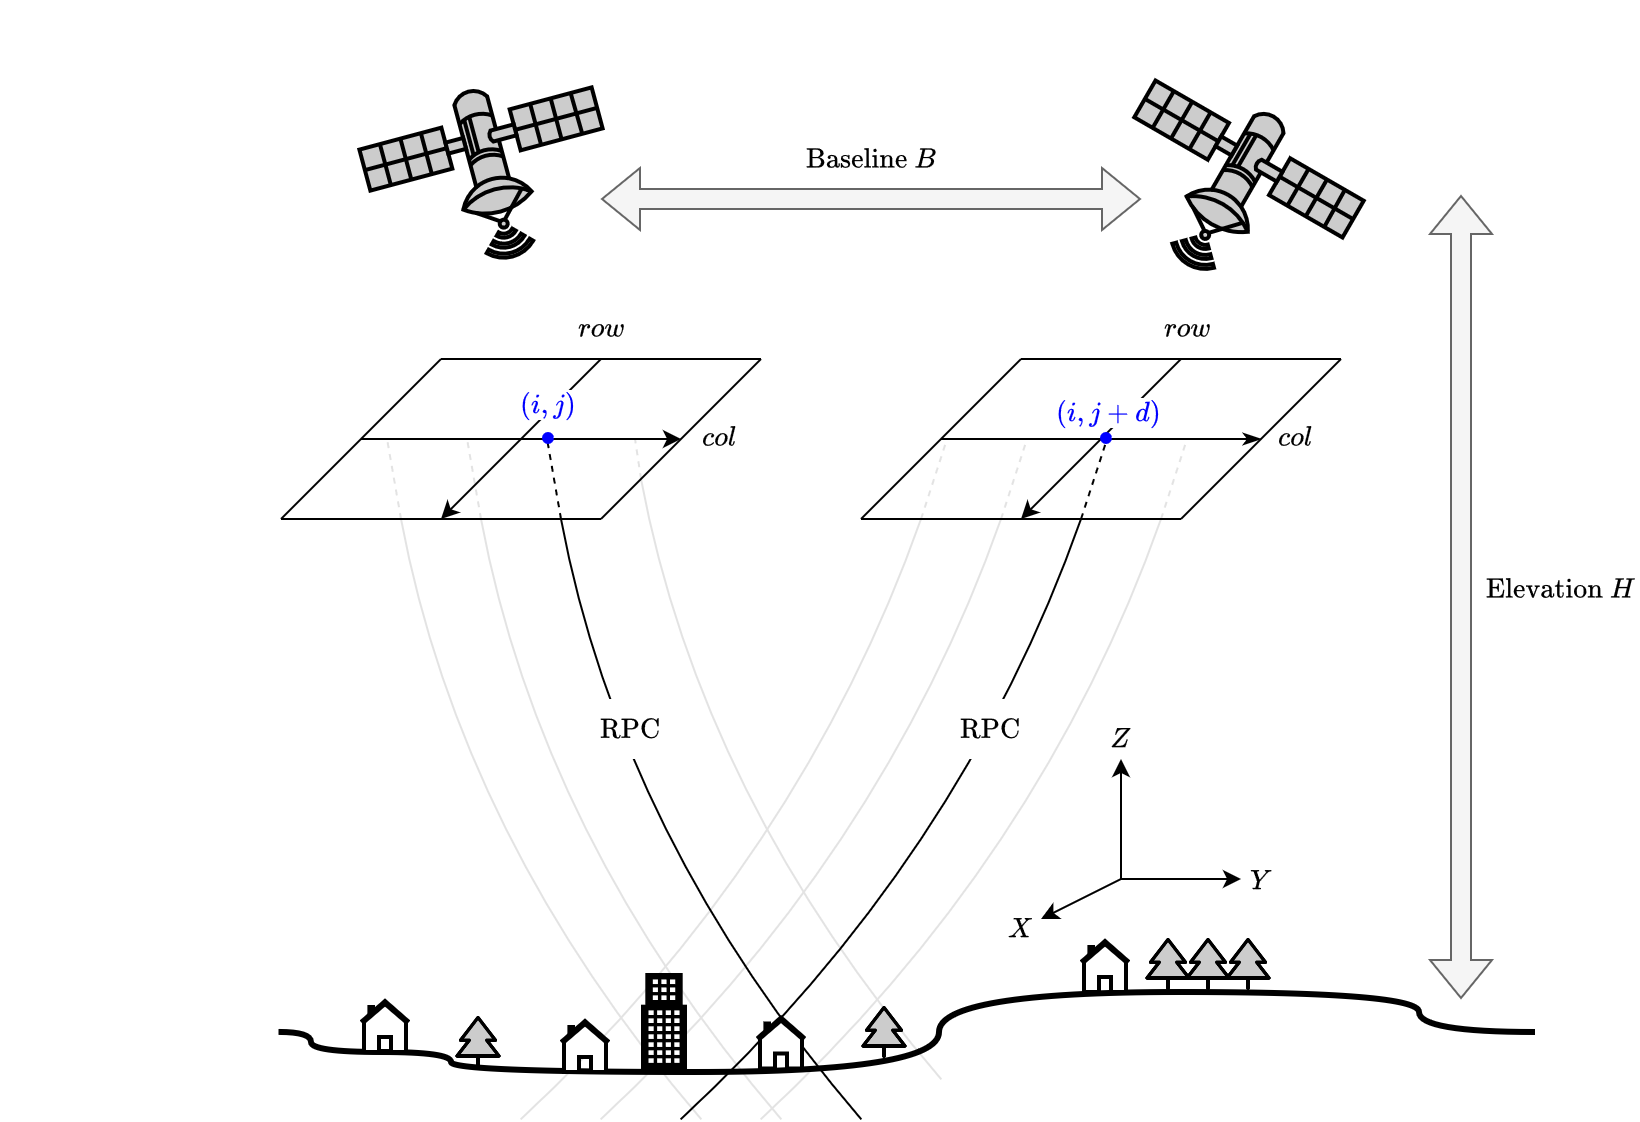
\includegraphics[width=0.8\linewidth]{Images/Chap_1/RPC.png}
    \caption{Triangulation of the position of a point using RPC models}
    \label{fig:RPC}
\end{figure}

Formally, \acrshort{rpc} are defined as rational fractions of polynomials:  
\begin{eqnarray}
    \RPC:\mathbb{R}^3 &\rightarrow&\mathbb{R}^2\nonumber\\
    (X,Y,Z) 	&\mapsto& \left(\frac{Num_{row}(X,Y,Z)}{Den_{row}(X,Y,Z)}, \frac{Num_{col}(X,Y,Z)}{Den_{col}(X,Y,Z)}\right)\nonumber\\
    &\mapsto&(row,col)\label{eq:rpc}
\end{eqnarray}
where $Num_{row},~Den_{row},~Num_{col}$ and $Den_{col}$ are the numerators and denominators for rows and columns respectively, expressed as polynomials with a maximum order of $3$:
\begin{eqnarray*}
    Num_{row}(X,Y,Z) &=& \sum_{i=0}^3~\sum_{j=0}^{3-i}~\sum_{k=0}^{3-i-j}a_{ijk}X^iY^jZ^k\\
    &=& a_{000} + a_{100} X + a_{010} Y + a_{001} Z + a_{110} XY + a_{101} XZ \\
    &&+ a_{011} YZ + a_{200} X^2 + a_{020} Y^2 + a_{002} Z^2 + a_{111} XYZ \\
    && + a_{210} X^2Y + a_{201} X^2Z + a_{120} XY^2 + a_{102} XZ^2\\
    && + a_{021} Y^2Z + a_{012} YZ^2 + a_{300} X^3 + a_{030} Y^3 + a_{003} Z^3
\end{eqnarray*}
$Den_{row},~Num_{col}$ and $Den_{col}$ respectively possess different coefficients $a_{ijk}$. The order or indexing of $a_{ijk}$ may differ in the literature. For instance, they can be numbered from $0$ to $19$ or $1$ to $20$, and do not refer to the same indeterminate. \acrshort{rpc} are computed using reference ground control points.\commanue{Discute avec Daniel mais tu peux effectivement utiliser des poinst de contrôle pour fitter les ceoff mais dans le cas des segments-sols, ils utilisent le modèle physique et ensuite ils fittent sur ce modèle un modèle RPC pour les utilisateurs normaux.}

It has been showed in \cite{baltsavias_metric_1992} that RPC are well suited to be used for ortho-rectification and stereophotogrammetry, as they possess good accuracy and are computationally fast. For stereo photogrammetry, it is ofter required to use the inverse \acrshort{rpc} model. As \acrshort{rpc} encode a line of sight given an image coordinate, the use of an additional elevation coordinate is required to move from the image space to the object space (\ie to go from a 2D space to a 3D space). It can be a geoid modelling the Earth's surface, or a \acrshort{dsm} with higher resolution. Knowing the true elevation $Z$ of a pixel, we define the inverse model as:
\begin{eqnarray}
    \RPC^{-1}:\mathbb{R}^3 &\rightarrow&\mathbb{R}^3\nonumber\\
    (row, col, Z) 	&\mapsto& (X,Y,Z) \label{eq:inverse_rpc}
\end{eqnarray}

An illustration on how RPC are used in stereo-photogrammetry is presented in \Cref{fig:RPC}. \commanu{c'est dommage de pas l'utiliser pour l'étape de triangulation. Ici, l'exemple le plus direct serait juste une loc sur ellipsoid ou DEM, ca evite au lecteur de penser autre chose (exemple image page accueil https://shareloc.readthedocs.io/)}

\section{Structure of the Stereophotogrammetry Pipeline}\label{sec:classical_stero_pipeline}
This section dives more into details of the inner workings of stereophotogrammetry\commanu{soit cohérent tout le long, 1 mot, 2 mots? pas pareil partout (dans l'intro t'as mis 2 mots)}, and presents the stereo pipeline mainly considered in this thesis. Photogrammetry is the science of deducing information from photographic images\commanu{ref ? un livre référence par exemple}. A sub domain of photogrammetry is stereophotogrammetry, which specifically consists in deducing 3D information from multiple photographic images. Although multiple stereophotogrammetry setups can be achieved, for instance using structured light \cite{scharstein_high-accuracy_2003} or different wavelength \cite{geng_rainbow_1996}, we focus here on the pipelines designed for processing satellite images, which are used and studied in this thesis. 

The main idea of stereophotogrammetry for satellite images and other 3D pipelines is to identify the parallax of objects between multiple images, and to deduce the distance between the object and the sensors from this displacement\commanue{Tu as le droit de mettre des schémas en plus tu risques d'en avoir besoin pour ta prez}. When expressed in pixels, the displacement is called disparity\commanue{si tu as un schéma plus loin mets une ref, sinon fait un schéma. C'est important que les termes que tu vas utiliser un nombre incalculable de fois par la suite soient bien définis}. To determine this disparity, the images must first be corrected from atmospheric effects (small clouds, aerosols, \etc) to go from top-of-the-atmosphere radiance to the actual light that illuminates the Earth surface \cite{hagolle_maja_2017}, called reflectance \comloic{je ne sais pas à quel point c'est vrai dans le cas de CO3D. Les acquisitions sont synchrones et le B/H petit. Je serai supris que en TOA les résultats soient très différents mais peut être. En tout cas je n'ai pas en tête de travaux qui le montrent.}\commanue{Alors si CO3D respecte le process standard la correction atmo c'est au niveau 2A donc tes images sont déjà projetées au sol donc on ne fait pas de 3D avec elles. Les images pour faire de la 3D c'est en général ce qu'on appelle de niveau 1B (correction radio et géo (recalage et modèle géométrique). A partir de 1C on projette au sol. Mais à vérifier avec David si CO3D utilise les niveaux de produits standards}. Many stereo setups\commanue{Alors là tu t'éloignes du satellite, je ne sais pas s'il ne faut pas le préciser. Ici quand tu parles de setups c'est les autres applications utilisant la 3D comme les voitures autonomes, les rovers sur Mars que tu as en tête} align their cameras in such a way that objects only move horizontally between images \cite{geiger_are_2012, scharstein_high-resolution_2014, keselman_intel_2017}. This allows to restrict the search space for pixel matches to a single row instead of the whole image. In a way, most people's eyes also present this alignment\commanue{je suis d'accord avec l'analogie mais la transition avec in a way c'est bizarre.}. When operating satellites, it is more complex to ensure that the sensors disposition will stay consistent\commanue{peut-être le tourner différemment, comme tu le mentionnes, habituellement dans les autres applications qui utilisent de la stéréo, les caméras sont montées de telle sorte à être dans la géométrie. Tu fais du principe d'acquisition satellite (qui défile) on n'est pas dans ce cas. C'est pas que c'est plus complexe. C'est que le mode d'acquisition ne le permet pas.}, thus requiring some pre-processing step to rectify images and ensuring that the displacement of an object only occurs horizontally (see \Cref{sec:epipolar_geometry}). Then matching pixels are determined by computing their disparity in a step called stereo matching presented in \Cref{sec:stereo_matching}\commanue{je suis en train de me dire que ce que tu racontes est très liée à la géométrie épipolaire. Mais que dans les faits les pipelines satellites font parfois le choix de reprojeter l'image de droite dans la géométrie de l'image de gauche donc corrélateur 2D car la mise en géométrie épipolaire est complexe. Donc peut-être que dans toute cette partie l'intérêt de la géométrie épipolaire doit être gardé pour plus tard et de rester haut niveau pour l'instant en disant seulement que l'étape consiste à trouver les pixels homologues entre deux images ou même pas car dans cette section, tu te limites à parler d'objets et non pas de pixels}\commanu{je suis d'accord, je ferais plus simple et ferait en 2 fois}. The 3D coordinates of the corresponding object are determined by computing the intersection between matching pixels' lines of sight (or best approximation if they do not strictly intersect). This results in a point cloud, where each point correspond to a match of two pixels\commanue{là on repart sur la notion de pixels donc soit tout ton paragraphe raisonne avec des objets dans les images soit tu parles de pixels dans les images. Mais si tu passes de l'un à l'autre c'est perturbant car les deux notions ne sont pas interchangeables}. The point cloud can be processed to remove outliers, and is then projected into a regular grid to obtain the desired \acrshort{dsm}. The following section dives more into details for the specific case of the CARS stereo pipeline\commanue{bah en fait non, dans la suite tu repars sur les pipelines existants. Donc je mettrais un peu d'ordre. Tu as fait un paragraphe très générique sur ce qu'est un pipeline 3D. Ce que tu as raconté ici, s'applique à tous, ça tombe bien c'est l'intro. Ensuite nouvelle section tu mentionnes les pipelines existants, tu peux fortement t'inspirer de ce que j'avais écrit pour ISPRS pour CARS. Tu auras peut-être besoin de la géometrie épipolaire. Et après tu enchaines sur CARS.}\commanu{en effet, mieux avec 1 général 2 pipeline existant 3 le notre cars, ca cleanera le meme feeling que manue entre ses deux sous sections}.

\subsection{Structure of the Stereo Pipeline}
Several stereo pipelines processing satellite images exist in the literature. We can think of NASA's \textit{ASP} \cite{shean_automated_2016}, IGN's \textit{MicMac} \cite{rupnik_micmac_2017}, Centre Borelli's \textit{s2p} \cite{franchis_automatic_2014}, DLR's \textit{CATENA} \cite{kraus_fully_2013}, Ohio State University's \textit{RSP} and \textit{SETSM} \cite{qin_rpc_2016, noh_surface_2017}\todoroman{Regarder "Metric Evaluation Pipeline for 3D Modeling of Urban Scenes" pour des comparaisons}. All those pipelines roughly possess the same structure, \ie pre-processing, images resampling in a convenient geometry for pixel matching, dense matching, triangulation and rasterization. Variations in those pipelines concern the different preprocessing steps (bundle adjustment, histogram equalization), the type of geometry used, the dense matching algorithms available \etc\commanue{Donc pour un chapitre de thèse va falloir plus détailler, je suis sure que j'ai mis plus d'info dans la publi de CARS ;) Il faudrait ajouter par rapport à ce que j'avais moi, c'est si certains pipelines gèrent ou non les incertitudes. Je n'avais pas regardé ce point à l'époque. Sans parler d'incertitudes, tu as peut-être a minima des flags qualité qui permettent au moins de dire ce résultat-là on regarde même pas}\commanu{et du coup, je découperais: une partie à part état de l'art des satellite stereo pipeline + une partie dédiée sur cars, revoir ta structure pour aider le lecteur} We will focus on the CARS pipeline used in this thesis, developed by CNES \cite{michel_new_2020}. A schematic of the different steps of the pipeline are presented in \Cref{fig:cars_pipeline}.
\todoroman{Insister sur le fait que CARS est tout automatique, y compris sur les cartes de performances à grande echelle. A voir avec Sylvia comment les DEM de l'IGN ont une carte de perf, et si oui si elle est pas manuelle}

\begin{figure}
    \centering
    \includegraphics[width=\linewidth]{Images/Chap_1/CARS_pipeline_detailed.png}
    \caption{Different steps of the CARS pipeline}
    \label{fig:cars_pipeline}
\end{figure}
The CARS pipeline works with grayscale images, but colored images (for instance pansharpened image) can be provided alongside the grayscale image\commanue{alors petite précision, Pandora ne fait de la corrélation que sur une seule bande. Donc CARS en général utilise les images PAN car plus résolues et ensuite complète sa sortie avec des infos issues du RGB. Donc je dirais plutôt que CARS (à cause de l'étape de corrélation) travaille majoritairement en mono-bande. Après si on envisage des étapes où on se sert du RGB par exemple pour faire de la classif ou pour filtrer, on pourrait avoir une plus grande utilisation de l'information provenant de plusieurs bandes}\commanu{je sais pas si c'est central en effet. a la lecture, ca donne l'impression que c'est important alors que c'est un peu annexe: ici tu présentes surtout les grandes étapes et les grandes lignes de fonctionnement du pipeline. La color peut etre un sujet intéressant mais annexe à ta problématique, attention digression comme vu par manue}. The grayscale pixels will be used in the pipeline\commanue{car les PAN sont plus résolues pour les images Pléiades. Pour CO3D on prendrait la bande verte car 2 fois plus de pixels}, but the colorimetric information will be kept until the final DSM, thus providing an ortho-rectified image\commanue{C'est pas faux mais il faut que tu fasses attention à toutes ces petites remarques que tu ajoutes et qui peuvent perdre le lecteur. As-tu besoin de parler les images orto RGB? Si oui, vraiment maintenant ou peut-être au moment de la rasterisation}.\commanue{Donc là voir remarque précédente, mais je mettrais ici clairement ce que c'est que les inputs de CARS : image en géométrie capteur mono-bande avec un modèle de prise de vue.}

\subsection{Resampling in Epipolar Geometry}\label{sec:epipolar_geometry}
The first step of the CARS pipeline is to resample the stereo acquisitions into a convenient geometry to carry out the dense matching\commanue{alors dans l'intro de cette section (qui es utile pour poser les termes), tu n'as jamais dis dense matching. Tu as juste parlé de matching (j'ai vérifié) donc dis juste matching entre les pixels. Tu expliqueras le terme dense dans l'étape de matching à proprement parlé}. This geometry is the epipolar geometry \cite{cnes_imagerie_2008}, which is constructed so that each line of an image follow the movement of the satellite, \ie the objects move only horizontally between the reference and secondary stereo images. This will\comloic{pourquoi will?} greatly facilitates the dense matching\commanue{juste matching} as the search space for a match is only limited to a one dimensional space instead of a two dimensional space around the pixel\comloic{la fin de la phrase est peut être pas utile}. A first approximation\commanue{pourquoi first approximation?} of the epipolar geometry can be computed using the respective geolocation models of both images $\RPC_1$ and $\RPC_2$. Indeed, given the altitude $Z$ of the object represented by pixel $(row_1, ~col_1)$ in the reference image, then\comloic{then pas utile} we can deduce its ground location $(X, ~Y, ~Z)$ using $\RPC_1^{-1}$. The position in the secondary image of those coordinates\comloic{là on ne sait pas trop si tu parles de la représentation du pixel (row,col) il y a deux phrases ou de la groud location} can then be retrieved using $\RPC_2$. In short, we found the secondary coordinates $(row_2,~col_2)$ of a pixel $(row_1,~col_1)$ in the reference image given an elevation $Z$\comloic{C'est pas limpide. Je vois comment ça marche dans ma cars mais là en te lisant je suis pas convaincu de l'ordre des opérations / explications}: 
\begin{equation}
    (row_2,~col_2) = \RPC_2\circ\RPC_1^{-1}(row_1, ~col_1, ~Z)\label{eq:epipolar_transfer}
\end{equation}
By varying the altitude in the range of considered elevations $[Z_{min},~Z_{max}]$, $\RPC_2\circ\RPC_1^{-1}$\comloic{tu peux la nommer f2->1 et préciser que c'est la fonction de colocalisation 2 vers 1} provides a characterization of the parallax between images. The lines described by $\RPC_2\circ\RPC_1^{-1}$ are thus the epipolar curves for the reference image\commanue{Tel que tu l'expliques, c'est plutôt la transformée d'une ligne de l'image de gauche par la composition des fonctions de RPC qui te donne la ligne épipolaire correspondante dans l'image de droite. Donc effectivement en faisant ça tu obtiens la ligne dans laquelle faire ta recherche. Mais il faudrait ajouter que c'est juste inutisable dans la pratique. On passerait son temps à faire des locs. Ce qu'on recherche c'est une transformation pour rééchantilloner les images}. Similarly, $\RPC_1\circ\RPC_2^{-1}$ provides the epipolar curves for the secondary. The range of considered elevations $[Z_{min},~Z_{max}]$ can be determined with a low resolution digital elevation model\commanue{pour faire une loc inverse tu as besoin d'une élévation donc n'importe quoi fait l'affaire.}. This is not constraining as a geoid of the Earth can be used, and there also exists open models such as the NASA's SRTM \cite{farr_shuttle_2007} ($30$m and $90$m of resolution between $-56\degree$ and $60\degree$ of latitude), or ESA's Copernicus DEM ($30$m and $90$m of resolution worldwide).  \todoroman{Parler aussi de la RGE Alti de l'IGN. regarder aussi s'ils ont un masque de perf}\commanue{Dans la suite tu repars sur le modèle pinhole. Donc cette partie sur le RPC on a l'impression que c'est pas fini. Peut-être commencé par parler du pinhole. C'est un modèle simple, c'est facile de calculer la transformée en géométrie épipolaire. Le souci c'est que le modèle pinhole n'est pas valide sur toute l'image mais localement. D'où l'utilisation du RPC mais les RPC ne permettent pas une formule analytique. Donc on passe par une grille de transformation. Et on utilise des compositions de fonctions de loc (et pour la fonction inverse on a besoin d'une hauteur).}

\begin{figure}
    \centering
    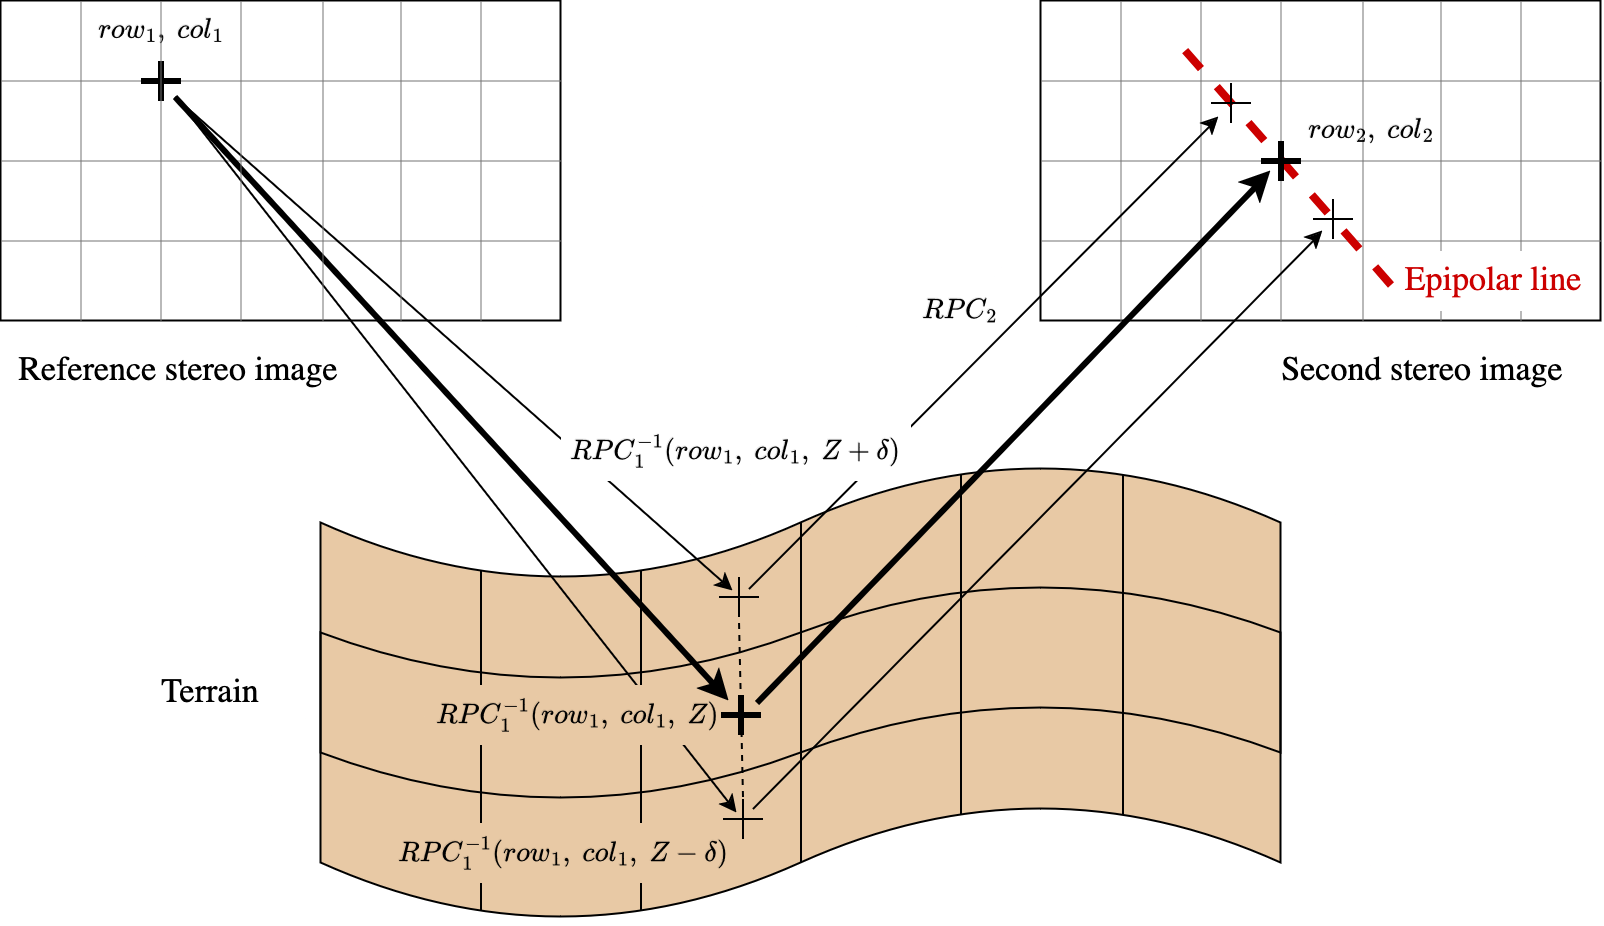
\includegraphics[width=\linewidth]{Images/Chap_1/epipolar_lines.png}
    \caption{Computation of an epipolar line for a pixel using small height variations}
    \label{fig:epipolar_lines}
\end{figure}

Captors using a pinhole camera model have a perfectly defined epipolar geometry, modeled by an affine transform \cite{hartley_multiple_2004}. This not true for push-broom sensors \cite{morgan_epipolar_2004}, but other models exist allowing to compute such a geometry \cite{oh_piecewise_2010, de_franchis_stereo-rectification_2014, koh_unified_2016, michel_new_2020}\commanue{Alors je mettrais la remarque en premier. Si on utilise un modèle simple pour décrire le modèle géométrique donc du pinhole c'est facile de faire le passage en géométrie épipolaire. Le pb c'est que le modèle pinhole n'est pas valide sur l'intégralité de l'image. Donc il faut l'appliquer par morceau, c'est ce que fait S2P. Résultat, tu as des effets de tuilages sur ton image. Ici on cherche une méthode pour passer en géométrie épipolaire en utilisant direct la précision du RPC. Alors tu cites la publi ISPRS de CARS mais justement on ne passe pas par du pinhole}\comloic{je rajouterai que ça va un poil vite. Quand tu dis qu'il existe d'autres modèles pour calculer la géométrie épipolaire tu passes un peu sous silence que ce sont des approximations, et justement la complexité dont on hérite avec des acquisitions de l'espace et des capteurs VHR principalement pushbroom, c'est qu'on ne peut pas exprimer la géométrie épipolaire de façon exacte sur l'ensemble du produit. Ensuite tu cites plusieurs papiers, il est important de noter ce qui distingue CARS des autres et notamment de la référence s2P (réf car IARPA winner tout ça tout ça). Dans s2p on a fait une approximation locale du modèle de caméra par un modèle type pinhole donc on peut réutiliser les algos de la computer vision à l'échelle d'une tuile sous réserve qu'elle soit petite. Dans CARS on cherche une représentation globale que l'on va exprimer par une grille de déformation qui fournit pour chaque point de la géométrie épipolaire sont équivalent dans la géométrie capteur.}. In the CARS pipeline, \cref{eq:epipolar_transfer} is evaluated with an elevation $Z$ extracted from the low resolution elevation model, and for small variations of altitude $Z\pm\delta$\commanue{alors je connais le principe mais là j'avoue que c'est pas clairement précédément tu as dit que tu pouvais avoir la ligne et là tu expliques que tu le fais localement. J'aurais tendance à renverser l'explication. Comme on ne peut pas avoir une trasformation analytique, on recherche une grille et voilà comme on évaluer chaque point de la grille.}. Those three points allow to compute the direction of epipolar lines for every pixel of both images as in \Cref{fig:epipolar_lines}\commanue{C'est un peu rapide. Comme on ne peut pas avoir une transformation en géométrie épiplaire qui peut s'écrire simplement via une transformation matricielle comme pour du pinhole. On décide d'exprimer la transformation par une grille que l'on peut prendre avec un pas assez large vu que les variations sont assez basse fréquence}. This method generates what is called an epipolar grid $g_{e1}$ joining every epipolar coordinate $(row_e, ~col_e)$ to its position in the reference image $(row_1, ~col_1)$:
\begin{align}\label{eq:epipolar_grid}
    g_{e1}(row_e, ~col_e) = (row_1, ~col_1)
\end{align}
A similar grid $g_{e2}$ is determined for the secondary image, which is actually computed jointly with $g_{e1}$. Those grids also use the low resolution elevation model\commanue{l'approche nécessite une altitude pour faire la loc inverse mais tu pourrais utiliser une altitude constante et la technique fonctionnerait. Si on utilise un DSM basse résolution c'est que cela permet de limiter l'intervalle de recherche.} to determine which altitude corresponds to a null disparity\commanue{Moi je tournerais plutôt la phrase qu'avec cette méthode par construction la disparité nulle correspond à l'altitude du DSM utilisé}\comloic{+1, c'est pas construction, tu peux amener ça de façon anecdotique, en gros c'est dans cette géométrie épipolaire là, puisqu'on pourrait en créer une autre, que la disparité nulle correspond à Z, où Z est censé être le Z dont tu parles plus haut et autour duquel tu ajoutes +/- delta, tu pourrais de Zcoarse ou Zdem. Enfin je veux dire, tu parles de Z en disant qu'il est extrait du low resolution elevation model mais on pourrait penser à un scalaire qui aurait au moins une occurence dans le low res elevation model, et peut être qu'il faudrait low res digital elevation model pour garder le lien avec DEM que tu présentes plus haut}. After the dense matching step, a disparity of $0$ would mean that the object has the same altitude than that of the low resolution elevation model. For more details on the way epipolar grids are computed, we refer to \cite{michel_new_2020}. Using those grids, it is possible to resample the reference and secondary images in their respective epipolar geometry. 

Because the geolocation models\comloic{c'est un termes que tu n'utilises que deux fois dans le manuscrit et je dirai qu'on pourrait l'introduire un peu mieux peut être pour ceux qui n'ont pas l'habitude de manipuler des images satellites. Peut être que dans le 1.3 le titre est trop vague, et le contenu fait un peu commercial plus que scientifique par moment. Je pense que tu pourrais y exposer plutôt des notations et des principes un peu originaux pour ceux qui découvrent l'image satellite mais sont qd mm intéressés par la thèse parce que par ailleurs ils font du stereo matching. Par exemple avant de parler des RPCs ou quoi faudrait introduire les systèmes de coordonées peut être. A la limite juste ECEF et UTM mais de quoi faire intervenir les notations X,Y, lon, lat, Z et h et les fixer pour le reste du manuscrit. Et ensuite seulement aborder les modèles géométriques et les RPCs et donc les loc directe et inverse. D'autre part à partir du 1.3 on parle souvent de DEM et d'intersecter un DEM du coup mais on parle pas du référentiel du DEM, en gros le Z du DEM il est par rapport à quoi ? faut faire intervenir géoide et ellipsoide je pense. Ou alors je vais trop loin mais là disons qu'on aborde tout ça très vite dans les premiers sous chapitre de cette section. Ensuite tu peux aborder les modèles de caméra utilisé dans le spatial un peu comme tu le fais mais sans le mélanger avec les RPCs, faudrait structurer avec un chapitre sur les syst de coord, un sur les modèles de caméra, un sur la géo d'acquisition en 3D qd même avec le b/h, avec le termes "nadir" peut être aussi, et ensuite les RPCs ou quoi)}  have a limited precision, there might be a misalignment left in the epipolar grids. To correct this error, a set of SIFT points \cite{lowe_distinctive_2004} is computed between the reference and secondary epipolar images. For every match, the difference between their rows is computed. The secondary epipolar grid is then corrected so that row differences are null on average. Once aligned epipolar grids have been obtained, stereo images can been resampled in epipolar geometry one last time so that \commanu{so that what ? à enlever ou finir la phrase}

\begin{remark}
    By computing the disparity for the set of SIFT points, it is possible to estimate the range of disparities to be considered in the dense matching step for a relatively low computation cost. We will see in \Cref{sec:triangulation} that there is an approximately\comloic{approximation?} allowing to simply convert disparities into an elevation using the $B/H$ ratio presented in \Cref{sec:stereo_matching}. Therefore, an approximation of the elevation of each SIFT match can easily be computed. A low resolution elevation model can then be derived from it, thus removing the need of an external model such as SRTM or Copernicus DEM.\commanue{Je ne suis pas sure que ça doit rester juste une remarque. MOn souci c'est qu'il y a plusieurs infos dans ta remarque. Premièrement les SIFT sont utilisés pour calculer l'intervalle de dispariaté,deuxième on peut convertir la disparité et troisièment on peut faire un DSM endogène. Donc la première partie de la remarque t'es surement utile. Le reste c'est à voir ou il faut faire plusiuers remarque.}\comloic{ouais c'est un paragraphe que tu pourrais avoir écrit la veille de la remise du manuscrit ça ;-) ça fait un peu, j'ai oublié deux trois choses qui rentrent pas dans le moule actuel donc je fais un patch. J'ai entendu dire que quand on fait un patch c'est un pb de conception si c'est pas un pb de temps ^^'}
\end{remark} 

Epipolar grids can also provide a good approximation of the disparity to altitude ratio $d_{alt}$ over the whole image, which can be used to determine the approximate $Z$ resolution of the DSM. It can also convert disparities into height as we will see in \Cref{sec:uncertainty_pandora}\commanue{Alors là je ne suis pas de comprendre le lien direct entre grille épipolaire et disparité}. 

\subsection{Stereo Matching}\label{sec:stereo_matching}
\subsubsection{Different Approaches}\commanu{pas sur que tu aies besoin de ce titre de soussoussection, j'enleverais}
Dense matching\commanue{je pense qu'il faut que tu prennes une phrase pour expliquer pour quoi on parle de dense matching. C'est assez typique de la télédétection où on fait du matching sparse pour recaler et dense pour la 3D. Donc je mentionnerais que l'on parle de dense car on réalise le matching sur l'ensemble de pixels} can be performed once epipolar images have been computed. As stereo matching is an important problem is\commanue{in?} computer vision, multiple algorithms have been proposed to compute a dense disparity match\commanue{c'est bizarre l'association de terme.}. Dense matching algorithms can be broadly classified into two categories: classical approaches following the steps outlined by Scharstein \etal \cite{scharstein_taxonomy_2001}, and deep-learning based methods \cite{laga_survey_2022}.
\begin{remark}
	In the domain of stereo matching, the reference image is often referred to as the \textit{left} image, and the secondary image is the \textit{right} image.
\end{remark}

Recently, deep-learning methods have been greatly improving\commanu{bizarre en anglais, je mettrais have greatly improved, sinon ce serait have been improved mais marche pas} the results of stereo matching algorithms \cite{tosi_survey_2024}\commanue{il faudrait que tu précises, tu parles de la stéréo en général et/ou de la télédétection}. Best results on famous benchmarks have been obtained using 2D an 3D convolution neural networks \cite{guo_openstereo_2024, liu_playing_2024}. Those deep-learning approaches often face generalization challenges, particularly when applied to images that differ from their training datasets. It is especially true in the case of satellite imagery \cite{mari_disparity_2022, jiang_rethinking_2024}, as there is a large variety of landscapes and sensors to consider, landscapes change with the seasons, and radiometry can also vary greatly between two acquisitions\commanue{je me dis que MCCNN c'est du deep learning mais c'est juste une étape donc quand tu parles de méthodes DL tu entends méthodes full DL ou non ? Si c'est le cas il faudrait le préciser.}. Many datasets are available for stereo processing, especially for autonomous cars \cite{geiger_are_2012, geiger_vision_2013}, but it is harder to come across open satellite datasets due to the costs and copyrights of satellite images, even if more datasets tends to be released \cite{bosch_semantic_2018, le_saux_data_2019, huang_urban_2022}\commanue{Les idées sont là mais l'ordre est pas évident. Soit tu expliques que les techniques DL notamment pour les voitures autonomes trustent les meilleurs perfs, car il y a bcp de datasets que la généralisation se passe bien puisqu'au final la structure de l'image varie peu. Et ensuite tu passes à la télédétection et là tu expliques que c'est plus mitig. Même si ces méthodes obtiennent de très bons résultats en télédétection, elles génralisent mal car les paysages sont très voire trop diverses, et en plus la création de VT est difficiles}. Obtaining ground truth data for satellite imagery is also challenging, as airborne campaigns are costly and often need to cover large areas to match satellite acquisitions\commanue{Oui c'est vrai que une acquisition LIDAR est chère. Mais c'est surtout que générer le jeu de données : aligner les données hétérogènes est un enfer et que tenir comptes des différences entre les acquisitions est un casse-tête et aussi passer le lidar en géométrie épipolaire}. All those factors make the training of a performing and generalizable network for satellite imagery quite challenging. Even though deep stereo algorithms will probably end up by replacing cost-based methods in future years\commanu{tu n'en sais rien et ca décrédibilise ton approche de thèse pour rien, donc à tourner plus positivement. Tu montres avant que ce n'est pas du tout sur. donc justifie plutot que l'approche de ta thèse est tout à fait logique et argumenté}, we will not focus on deep end-to-end algorithms\commanue{c'est ici que tu mentionnes le end-to-end} in this thesis and instead restrict ourselves to so-called \textit{classical} methods used in satellite stereo pipelines. Those methods have the advantage of relying on an extensive literature on the subject, and implementing new features (for instance a new optimization strategy or a new cost function) is usually easier and does not require to re-train the whole network\commanue{en même temps MCCNN c'est du DL donc... En fait le truc c'est que les méthodes end-to-end en plus de mal généraliser actuellement (on peut se dire que peut-être ce verrou peut sauter à terme) sont des boîtes noires donc mettre de l'explicabilité comme tu le fais ça me paraît pas être adapté. Il faudrait que le réseau apprenne la disparité et son intervalle d'erreur en même temps. Je pense que cette phrase est à mettre dans le paragraphe suivant.}\comloic{je pense aussi que l'objectif de la thèse rend compliqué l'utilisation d'algo IA end to end. C'est pas seulement landscape et sensors to consider, il y a le b/h, la résolution des images, les angles de dépointages à b/h équivalent etc. et le fait que la plupart de ces algos subissent un entrainement supervisé. Vu qu'on ne sait pas estimer la disp parfaite entre deux images avec des algos non IA (sinon à quoi servirait l'IA) on peut pas générer la VT donc on prend une source exogène qui fait office de VT mais qui présentent des incohérences. Tu peux qd même ouvrir sur le fait que des algos entrainés de façon non supervisée pourraient s'affranchir de certaines problématiques citées mais c'est pas encore mature et c'est pas écolo or CO3D c'est du low cost}.

Classical approaches usually encompass the following steps \commanu{+described in following subsections, pour aider à la transition?} \cite{scharstein_taxonomy_2001}\commanue{je ferais une liste avec item, tu n'es pas limité en nombre de pages.}: matching cost computation, cost aggregation, disparity computation, and disparity refinement. \Cref{fig:stereo_matching_pipeline} illustrates those different steps. In this thesis, we will mainly consider classical approaches\commanue{tu l'as déjà dit dans le paragraphe d'avant.}, specifically as the CARS pipeline uses a dense stereo correlator called Pandora, developed at CNES (\url{https://github.com/CNES/Pandora})\commanue{J'ajouterais une phrase pour dire que maintenant tu vas détailler les étapes}\commanu{et à la lecture des étapes d'après on ne retrouve pas celle de ton schema général, notamment sur SGM pas mis dans le pipeline. Pour quelqu'un qui connait pas trop, c'est confusing. Donc j'introduirais bien les memes étapes "générales" que tu décris après}.

\begin{figure}
	\centering
	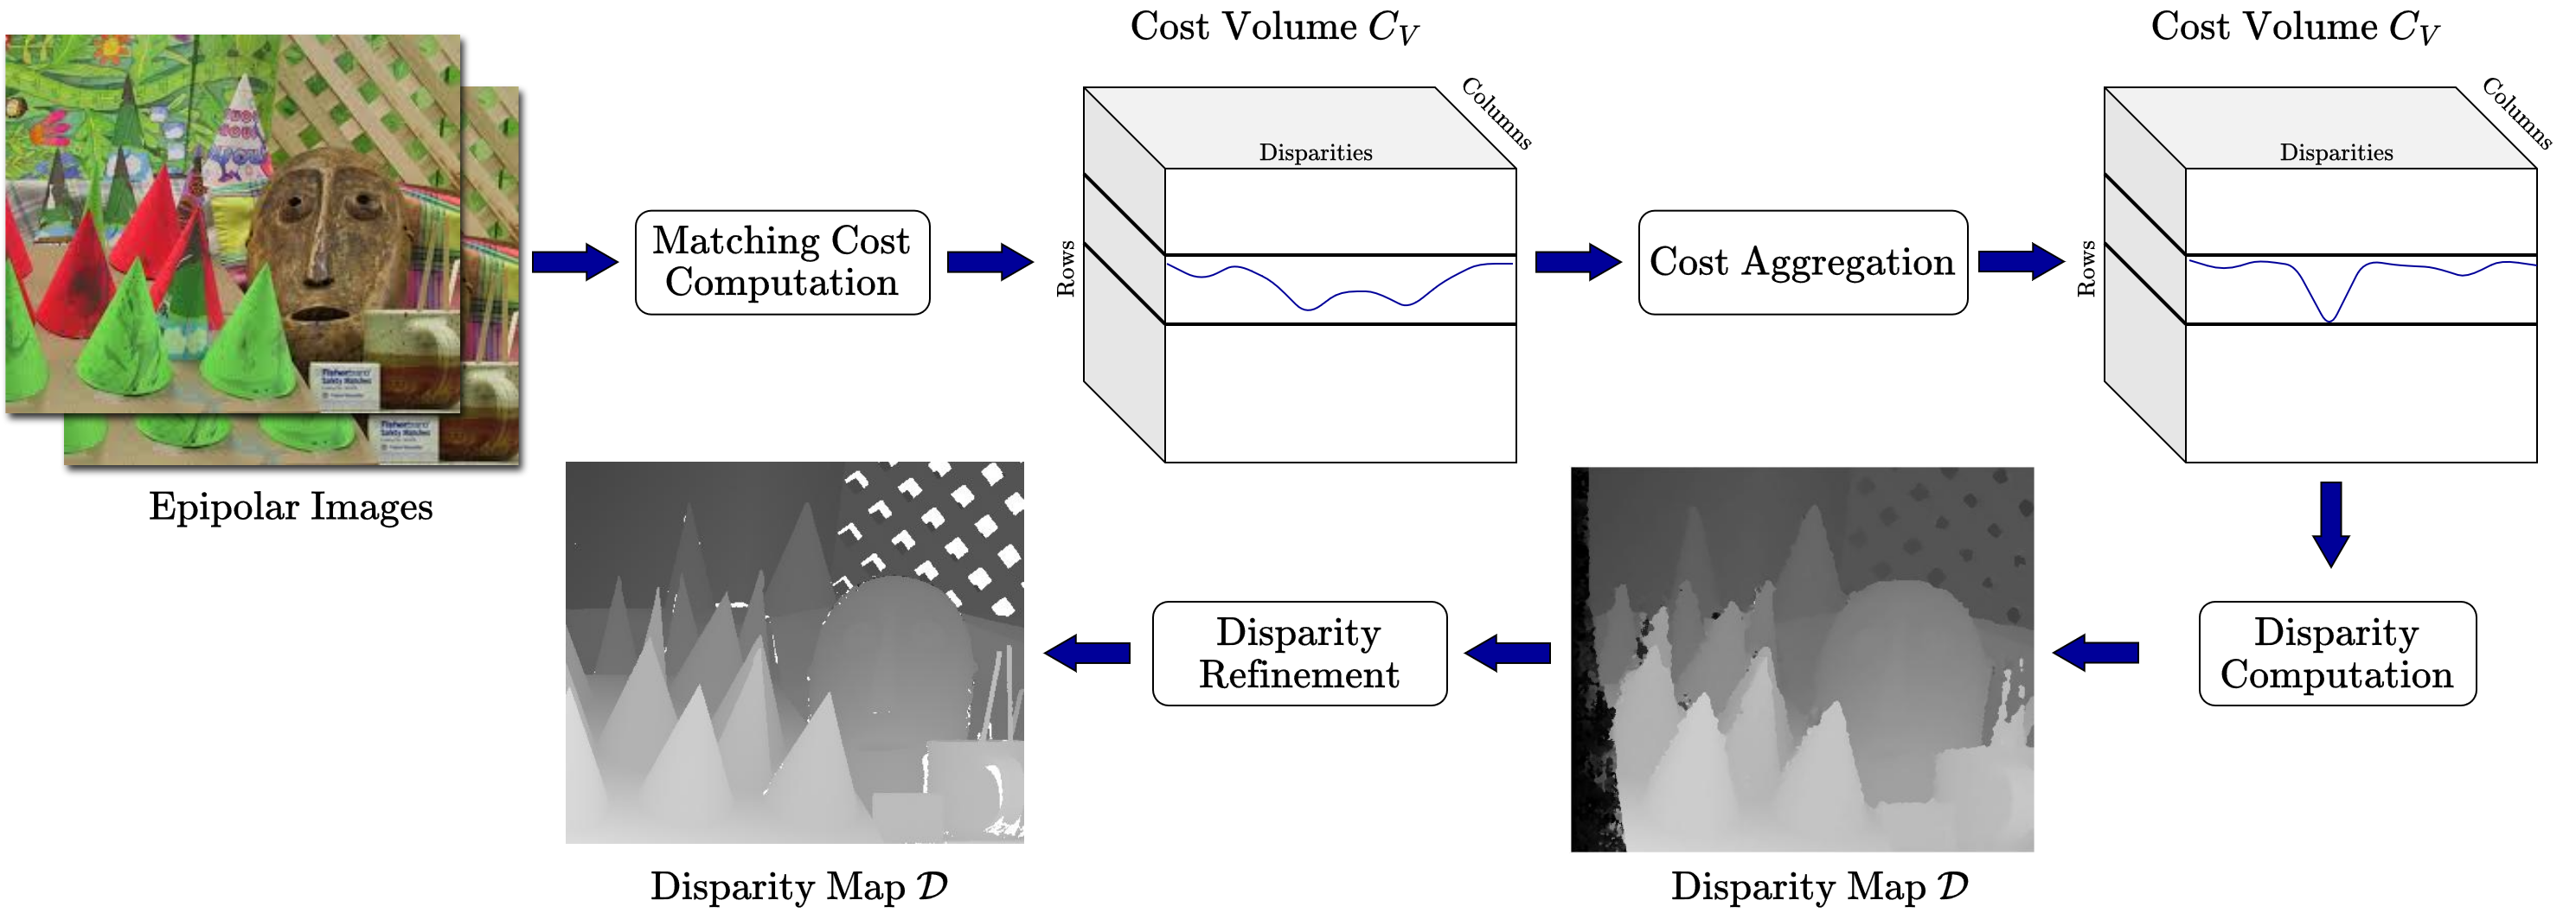
\includegraphics[width=\linewidth]{Images/Chap_1/stereo-matching_pipeline.png}
	\caption{The different steps of classical dense stereo-matching algorithms.}
	\label{fig:stereo_matching_pipeline}
\end{figure}

\subsubsection{Cost Volume Computation}\label{sec:cost_volume_computation}
The cost volume computation can be described as follows: given a range of considered disparity, the cost of matching every pixel of the reference image to every pixel in of the secondary image in the disparity range is stored in an array of data called cost volume (\Cref{fig:cost_volume})\commanue{Avant de dire que c'est stocké dans un cost volume, je dirais que le coût représente la similarité entre deux pixels des deux images. Dans cette première phrase tu mentionnes beaucoup le terme de coût }. The matching cost is evaluated using a cost function, which is a mapping $f$ from subsets of the left and right images to $\mathbb{R}$\commanue{Tu peux peut-être rajouter que la focntion de coût est là pour donner un score sur la similarité entre les pixels de deux images avant de te lancer dans les exemples}. Example\commanue{C'est bizarre le terme example} \ref{ex:cost_functions} provides different examples of cost functions\commanue{Peut-être ajouter une définition générique de la fonction de coût avant de parler des exemples}.

\begin{example}\label{ex:cost_functions}
	Simple examples of cost functions include the Sum of Absolute Differences (SAD), the Zero Normalized Crossed Correlation (ZNCC)  \cite{hannah_computer_1994}, the CENSUS transform \cite{zabih_non-parametric_1994} and MC-CNN \cite{zbontar_stereo_2016}.
	
	Given two windows $W_L$ and $W_R$ from the left and right images, the SAD cost function is defined as follows:
	\begin{equation}
		f_{SAD}(W_L, W_R)  = \sum_i\sum_j | W_L(i,j) - W_R(i,j) |
	\end{equation}
	Low $f_{SAD}$ values indicate that the windows are similar, while high values indicate noticeable differences. A $f_{SAD}$ value of $0$ indicates that the windows are identical. This cost function is probably the simplest cost function one could imagine, and will be used to detail\commanue{le to detail est en trop à mon sens car tu as déjà une autre verbe après} in \Cref{chap:propagating}\comloic{juste used in chapter 4 to didactically} to didactically illustrate how uncertainty models can be propagated throughout a cost function. However, this cost function is not usually used\comloic{usually used? ;-) en gro c'est pas robuste à un bias radio entre les images ni un offset, or meme dans les conditions CO3D (et déjà c'est synchrone ou quasi et pas commun), tu as des objets imagé a la meme heure mais selon l'angl de prise de vue la radio peut différer donc SAD dans les chous}\commanue{in practice ?} in stereo matching algorithms as more efficient cost functions have been proposed since\commanue{tu pourrais juste préciser que ce n'est pas efficace car juste baser sur des différences radio}. It can be a fast and easy way to have a first estimate of similarities between multiple patches. The SAD can also be used for motion estimation and image/video compression \cite{richardson_h264_2006}.
	
	The ZNCC cost function is defined as the correlation coefficient between both images:
	\begin{equation}
		f_{ZNCC}(W_L, W_R)  = \sum_i\sum_j \frac{(W_L(i,j)  - \tilde{W}_L) (W_R(i,j)  - \tilde{W}_R) }{\sigma_L\sigma_R}
	\end{equation}
	where $\tilde{W}$ refers to the mean value of a window, and $\sigma$ its standard deviation. Negatively correlated windows would present a ZNCC value of $-1$ and positively correlated windows present a ZNCC value of $1$. Contrary to the SAD cost function, matching windows will be indicated by a high value of the ZNCC. It is thus not \textit{strictly} a cost function but rather a similarity function. It is not a problem, as multiplying $f_{ZNCC}$ by $-1$ will transform it into a cost function. Another formulation could be to say that the $ZNCC$ is a \textit{maxitive} cost function, in the sense where potential matches are found by searching for its maximum. Conversely, the SAD is a \textit{minitive} cost function in the sense where potential matches are indicated by a minimal cost.\commanue{Avantages? Inconvénients? Est-ce qu'on l'utilise? Non, ça présente pas mal d'intérêt notamment dans les zones homogènes mais pour CO3D on vise des trucs sympas en urbain vu que bon, l'argent il est là... donc il faut pas trop baver enfin adhérer, donc on préfère census}
	
	The CENSUS cost function\comloic{à l'oringe c'est un filtre, Census Filter, ça devient dans le langage commun une cost function juste parce que si tu l'applique à deux images et que tu ajoutes la distance de hamming bein ça marche bien} needs a bit more detailing\commanue{mon anglais pourri penche pour needs to be a little more detailed}\comloic{+1}. For a squared window $W$ with a side of $2n+1$ pixels, we first compare the value of each pixel of the window with the center pixel. This gives a binary string where $1$ indicates that the value of the pixel is superior to that of the center pixel. For instance if we consider the two $3\times3$ following windows $W_L, W_R$:
	$$
    \begin{bmatrix}
        155 & 133 & 97 \\
        80 & 110 & 132 \\
        100 & 102 & 120
    \end{bmatrix}
    \qquad
    \begin{bmatrix}
        175 & 153 & 133 \\
        100 & 130 & 152 \\
        120 & 135 & 125
    \end{bmatrix}
	$$
	Then comparing each of their pixel to the center of the windows will yield the following binary strings (expressed here as matrices):
	$$
    \begin{bmatrix}
        1 & 1 & 0 \\
        0 &  & 1 \\
        0 & 0 & 1
    \end{bmatrix}
    \qquad
    \begin{bmatrix}
        1 & 1 & 1 \\
        0 &  & 1 \\
        0 & 1 & 0
    \end{bmatrix}
	$$
	The cost function $f_{CENSUS}$ is finally obtained by taking the Hamming distance (\ie the number of different bits between those two strings:
	\begin{equation*}
		f_{CENSUS}(W_L, W_R) = 3
	\end{equation*}
	
	The CENSUS cost function compares relative intensity variations, it is thus less sensitive to variations of intensities between images, such as a change of exposure for instance. Similarly to the SAD, two similar patches will tend to have a low value.
	
	The MC-CNN cost function \cite{zbontar_stereo_2016} is using a convolutional neural network architecture to measure the similarity between patches\commanue{ça mérite un peu de schémas}\comloic{la partie convolutionnelle elle permet de décrire un patch, un peu comme un descripteur sift quoi, après il y a une mesure de similarity (cosine similarity) branchée derrière et une loss qui force la sortie du nn à tendre vers des patchs utiles pour le matching en particulier}. It was train on $11\times 11$ patches from stereo images from the Kitti \cite{geiger_vision_2013, menze_object_2015} and Middlebury \cite{scharstein_taxonomy_2001,scharstein_high-accuracy_2003,hirschmuller_evaluation_2007,scharstein_learning_2007,scharstein_high-resolution_2014} datasets. They first trained their network to compute a vector of features for each patch\commanue{Modèle siamois même réseau pour extraire les features entre les iamges}. They then trained a second network to compute the similarity measure between both feature vectors. They also proposed a so-called ``fast'' architecture, which directly computes the cosinus between both vectors, thus by-passing the need of a second network for similarity\commanue{Avec le cosinus simple produit scalaire donc}\comloic{ok tu précises des choses ici, mais du coup plus haut, au moment ou tu dis MCCNN c'est un CNN pour mesurer la similarité c'est pas trop ça... enfin faut choisir, MCCNN c'est soit un outil, celui du papier, soit un réseau de neurones mais qui ne sort pas une mesure de similarité il sort juste un descripteur à la sift}. As ZNCC, MC-CNN is a similarity measure\comloic{ok donc soit c'est une mesure de similarité, mais alors là c'est pas juste un convolutional neural network, c'est soit l'enchainement de deux cnn soit un cnn et une vraie mesure de similarité qui n'a pas besoin de MCCNN pour être une mesure de similarité d'ailleurs}, but can easily be converted into a cost function. Although it has been trained on stereo images of autonomous cars (Kitti) and stereo images of toys (Middlebury), it generalizes well to our satellite images\commanue{cite la publi de Véro et Loïc}.
\end{example}
	
Using the chosen cost function $f$, a cost volume $C_V$ is then evaluated by measuring the cost of matching every patch in the left image to every pixel in the right image in the given disparity range\commanue{ça ressemble bcp à l'intro, donc je pense que ton intro devrait démarrer par la fonction coût et ensuite tu embrailles comme tu le fais avec le cost volume}. The cost volume as thus three dimensions, namely rows, columns and disparity:
\begin{equation}\label{eq:cost_volume}
    C_V(row, ~col, ~d) = f(W_L(row, ~col),  W_R(row, ~col+d))
\end{equation}
where $W_L(row, ~col)$ is a window centered on the pixel at coordinates $(row, ~col)$ in the left image, and $W_R(row, ~col+d)$ is a window centered on the pixel at $(row, ~col+d)$ in the right image. We usually add some padding to the images to avoid problems near borders where the column $col+d$ would not be defined. Given a pixel in the left image $(row, ~col)$, matching cost values for every considered disparity form what is called a cost curvecurve. In theory, the correct disparity for a match is determined by finding the minimum of the cost curve (for minitive cost functions such as SAD or CENSUS). In the rest of this thesis, we will consider that a cost function is always minitive unless specified otherwise. In practice, directly determining correct disparities from the cost volume is not efficient as geometric structure of the scene is not yet taken into account\commanue{Je ne suis pas sure de comprendre. Tu veux parler du fait que sans optimisation on a pas de bons résultats ? C'est pas évident de voir ce que tu sosu-entends par prendre en compte la géométrie de la structure étant donné que c'ets justement ce qu'on cherche a estimé. Peut-être dire juste préciser le meilleur candidat donc approche locale sans tenir compte du voisinage des disparités ne donne pas des choses terribles et donc un exemple pour montrer que c'est très bruité.}. \Cref{fig:cost_volume} represents a cost volume, and one of its cost curves where potential matches have been highlighted\commanue{peut-être mettre cette phrase avant quand tu définis les termes. Ensuite tu pars sur des remarques pour revenir sur un schéma}. 

\begin{figure}
	\centering
	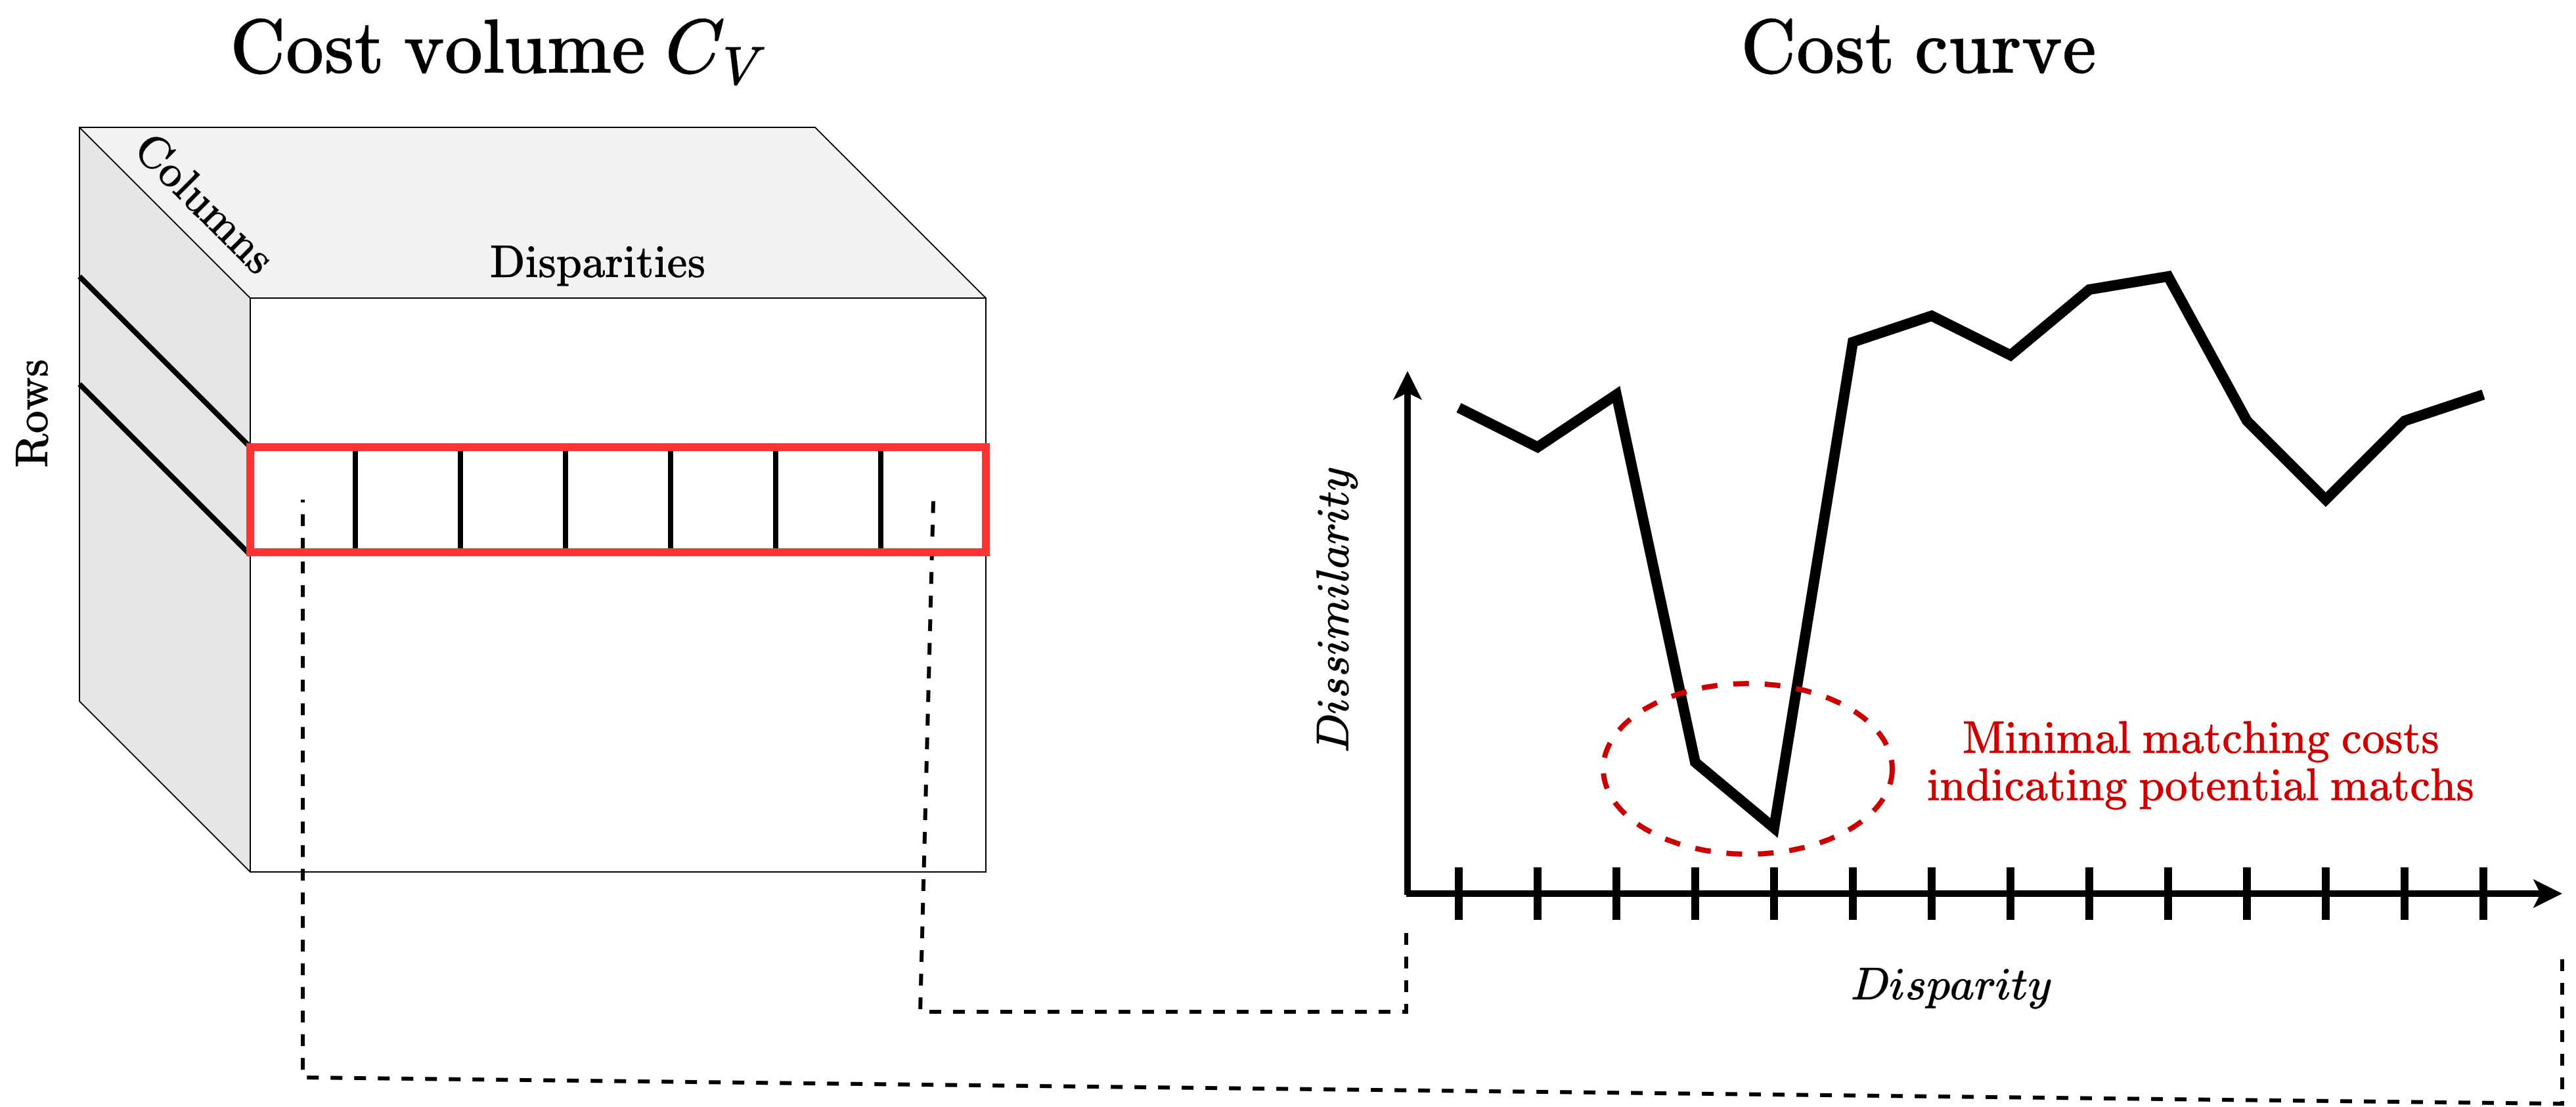
\includegraphics[width=\linewidth]{Images/Chap_1/Cost_volume.png}
	\caption{Matching cost volume and one of its cost curve}
	\label{fig:cost_volume}
\end{figure}\commanu{dans le texte de la figure: minimal matching cost indicating potential match, sans pluriel. ou sinon matchs-> matches}

The usage of windows\commanue{in the calculation of the cost function} allows to take into consideration the surrounding of pixels to better measure their similarity. However, window based approaches\commanue{ajouter peut-être: , mostly square-shaped,} also present the disadvantage of struggling to correctly identify matches near object borders \cite{hirschmuller_real-time_2002}. This is usually called an adherence effect, represented in \Cref{fig:adherence_window}\commanue{Pour montrer l'adhérence il te faut aussi un schéma en 3D pour que les gens comprennent bien ce que voit l'image de gauche et celle de droite. Après tu peux rester 1D pour que ce soit plus simple. Il te faut aussi (oui c'est relou l'adhérence) le résultat en terme de disparité pour montrer pourquoi on appelle cela adhérence}. In this figure, there are three objects represented with three different colors. Centered pixels of both windows do not match, contrary to the rest of the windows which are exactly the same. Sliding the right window in both directions would lead to higher matching costs, as the windows would be even more dissimilar\commanue{je ne suis pas sure de comprendre la phrase. L'adhérence c'est justement que tu vas te retrouver à trouver qu'à cause du voisinage tu vas pas associer le bon pixel. En général tu descends du building un peu plus tard que dans la réalité. En fait ce qu'il te manque dans ta figure c'est qu'est-ce qu'il faudrait associer comme bonne disparité et qu'est-ce que tu as associé en fait du fait de la fenêtre utilisée.}. This illustrates the fact that matching windows do not necessarily mean that the center pixels constitute a match. Other work have been proposing to use a spatial weighting \cite{kuk-jin_yoon_locally_2005}, segmentation \cite{hutchison_segmentation-based_2007}, windows with different shapes \cite{ke_zhang_cross-based_2009, buades_reliable_2015} to solve this problem. 
\begin{figure}
	\centering
	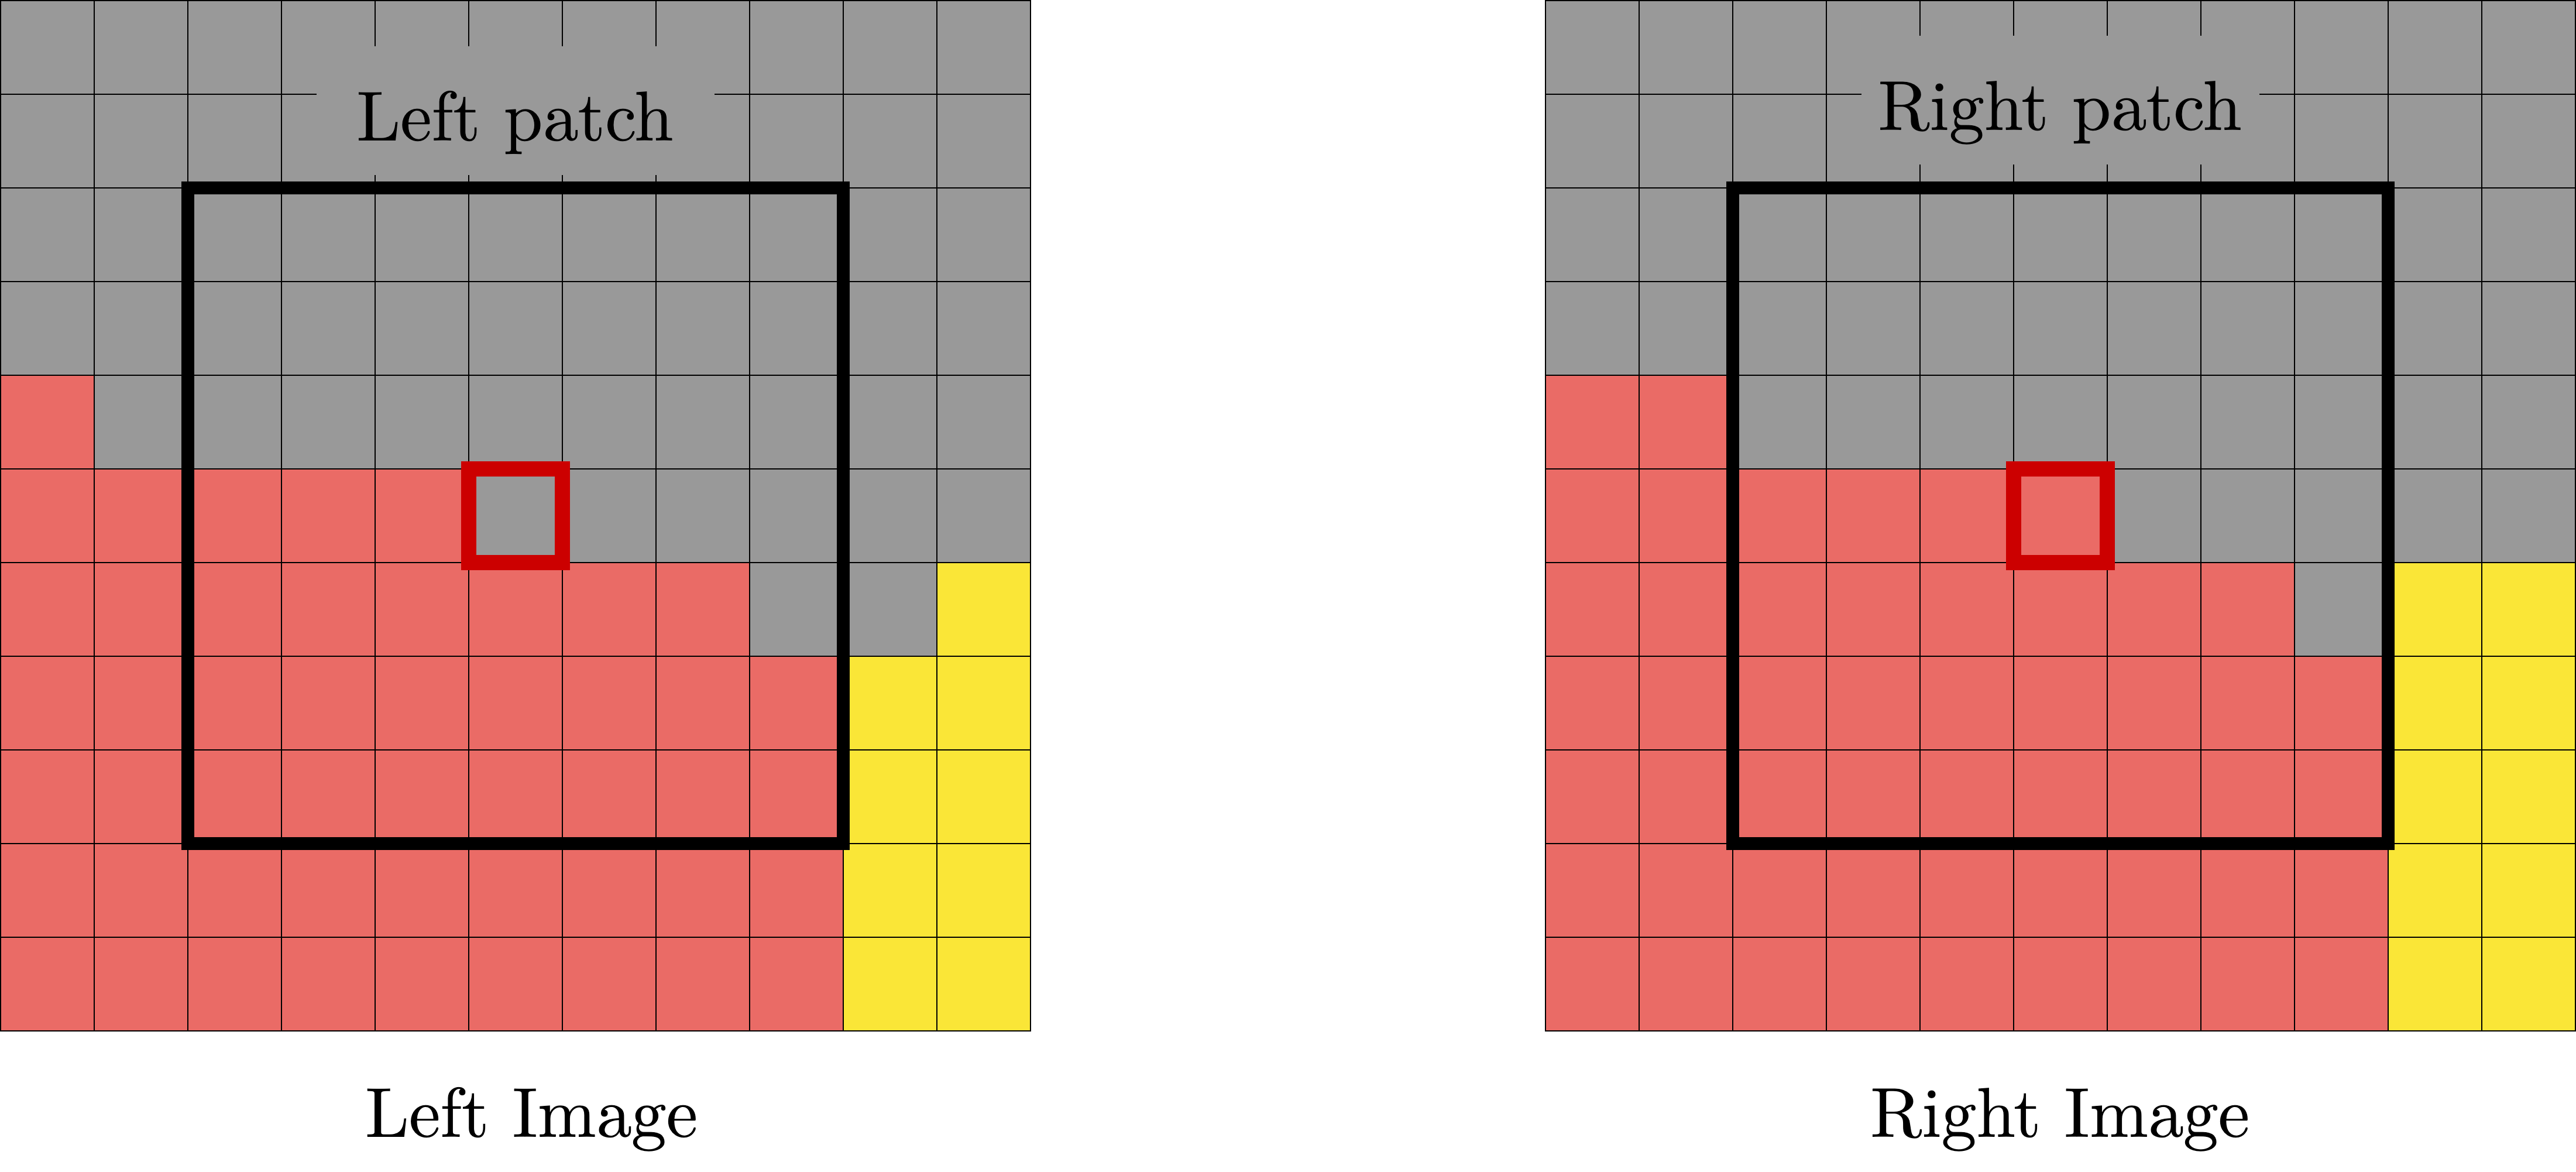
\includegraphics[width=\linewidth]{Images/Chap_1/Adherence_window.png}
	\caption{Adherence problem when comparing two patches between epipolar images}
	\label{fig:adherence_window}
\end{figure}

After computing the matching cost, information regarding the geometric structure of the scene\commanue{c'est pas ton meilleur choix de terme} can be incorporated in the cost volume. A first approach is to aggregate different parts of the cost volume. Usually, costs of pixels belonging to the same objects are aggregated using different methods for segmentation \cite{ke_zhang_cross-based_2009, ji_superpixel_2021}. This part is not always present in algorithms, as we will see next there exists regularization algorithms designed with the same purpose. 

\subsubsection{Semi Global Matching and Disparity Computation}
\commanu{comme dit au début de la partie dense matching, pas évident de retrouver l'ordre de présentation du début. etre cohérent avec le déroulé du début du dense matching, sinon pas évident de suivre pour un lecteur}
Computing the disparity map from the cost volume can be done in several ways. So-called local methods apply a direct \textit{winner-takes-all} strategy, where the $\argmin$ of every cost curve is kept as the selected disparity. This has the disadvantage on allowing multiple pixels from the right image to be matched to the same pixel of the left image\comloic{je vois pas trop pourquoi ça ne peut être le cas pour une méthode globale ? je rate un truc ?}. On the other hand, global method use the information contained in the cost volume to solve an optimization problem, where the objective is to compute the disparity map $\mathcal{D}$ minimizing an energy function expressed as follows:
\begin{equation}
    E(\mathcal{D}) = E_{data}(\mathcal{D}) + \lambda E_{smooth}(\mathcal{D})
\end{equation}
where $\lambda$ is a scalar for tuning the importance of the regularization term $E_{smooth}$. Usually, the data term is directly computed from the cost volume as:
\begin{equation}\label{eq:global_methods}
    E_{data}(D) = \sum_{row,~col}C_V(row, ~col,~D(row, ~col))\commanue{C'est pas le même symbole D que dans la précédente équation}
\end{equation}
The regularization term $E_{smooth}$ can take numerous forms, usually measuring if the neighbouring disparities possess similar values \cite{scharstein_taxonomy_2001}. Then a local minimum for this energy is found using various methods, such as Markov Random Fields \cite{boykov_markov_1998, sun_stereo_2003}, graph cuts \cite{kolmogorov_computing_2001} or minimum spanning trees \cite{zureiki_stereo_2008, qingxiong_yang_non-local_2012}. Those algorithms improves performances in comparison to local methods, but can be computationally expensive.

The most popular method is actually Semi-Global Matching (SGM) \cite{hirschmuller_accurate_2005}: it aims at incorporating regularization constraints to the cost volume similarly to global methods, in order to be processed\commanue{j'aurais tendance à mettre while being processed with relative low computational cost pour montrer que SGM cherche à avoir les avantages des deux côtés}\comloic{ouais parce que il y a aussi un cost volume dans de vraies méthode globale genre basées sur les graphes et résolue par komlogorov ou son copain donc là c'est surtout que c'est semi global parce qu'on résoud pas le problème initial on fait une modélisation simplifiée en réduisant tout ça a quelques chemins} like local methods. It is, in a way, in-between local and global methods. This is the method we will\commanu{j'aurais enlevé le will} use in the CARS pipeline for experiments in this thesis. In short, for each pixel, the SGM algorithm looks into neighbouring pixels recursively, and increases the cost of disparities that do not present a consensus\comloic{pas sur de te comprendre?} amongst neighbours \comloic{je pense que si tu veux être rigoureux tu dois présenter le CV comme un graphe, avec les noeuds qui sont le terme Edata c'est à dire les couts de similarité et les liens qui sont le termes Esmooth. Ensuite SGM dit simplement "je vais pas résoudre le problème dans sa globalité je vais le réduire à une dimension et répéter 4/8 fois ce job pour 4/8 directions}. Although the formulation of the SGM algorithm can be expressed in a few equations, understanding how its inner workings is more complex. We will first present its mathematical formulation in \cref{eq:sgm,eq:sgm_penalties}, and use \Cref{fig:sgm} to illustrate its effect on (a portion of) a cost curve. Formally, for every pixel $p=(row, ~col)$, the cost volume is explored in multiple directions as in \Cref{fig:sgm_directions}.

\begin{figure}
	\centering
	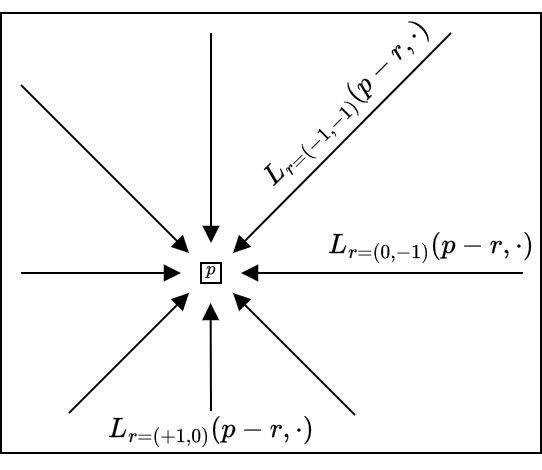
\includegraphics[width=0.5\linewidth]{Images/Chap_1/SGM_directions.png}
	\caption{SGM regularization with $8$ directions}
	\label{fig:sgm_directions}
\end{figure}

The cost is regularized for each direction $r$ to take into account the best disparity $d$ along that direction. A direction can be for instance $r=(0,~1)$, meaning that we will look at same row and travel to the right of the image when browsing direction $r$. Given two positive scalars $P_1<P_2$, the regularized cost $L_r$ along direction $r$ and at disparity $d$ is expressed with the following recursive formulation:
\begin{align}\label{eq:sgm}
    L_r(p,d) = C_V(p,d) + \min_\delta \left(L_r(p-r,~\delta) + R(d, ~\delta)\right)\commanue{elle est bizarre la formulation de SGM. Je comprends le $\delta$, c'est pas évident de retrouver la formule de l'article}
\end{align}
where $R(d, ~\delta)$ equals:
\begin{align}
    R(d, ~\delta) = &P_1\cdot\mathds{1}(|d-\delta|=1) + P_2\cdot\mathds{1}(|d-\delta|\geqslant 2) - \min_k L_r(p-r,~k) \label{eq:sgm_penalties}
\end{align}
Here, $\mathds{1}$ is the indicator function. The first term of \cref{eq:sgm} is the cost volume, which can be compared to $E_{data}$ in \cref{eq:global_methods}. The second term is similar to the regularisation term $E_{smooth}$. This term can be seen as the regularized cost $L_r(p-r, ~d)$ from the previous pixel in direction $r$, but shifted of $P_1$ for neighbouring disparities $d\pm1$, and of $P_2$ for further disparities. The term $\min_k(L_r(p-r,~k))$ prevents $L_r(p,\cdot)$ to diverge to very high values by ensuring that the minimum of $L_r(p-r,~\delta) - \min_k(L_r(p-r,~k))$ always equals $0$. \Cref{fig:sgm}\commanue{J'avoue que j'ai du relire le paragraphe plusieurs fois, j'ai un peu  de mal avec ta notation qui se veut très générique. C'est un peu le même prinicipe pour la figure. C'est ton choix donc à voir si ça parle plus aux autres.}\commanu{en effet pas évident. peut etre un exemple plus concret sur ce que ca permet de faire et donc de mieux comprendre la motiv de l'algo et donc l'algo in fine. mais pas évident de toute façon de bien l'expliquer} presents $L_r(p-r,~\delta) + R(d, ~\delta)$ for two different disparities $d$ and $d+1$ in the blue frame. The minimum of each curve $L_r(p-r,~\delta) + R(d, ~\delta)$ (blue arrows in the figure) are then added to the matching cost $C_V(p,d)$ to obtain the final regularized cost $L_r(p,d)$. Note that in \Cref{fig:sgm}, the minimum of $L_r(p-r,~\delta)+R(d+1, ~\delta)$ equals $0$, thus $C_V$ is unchanged for this disparity. This is because $d+1$ is the minimum of $L_r(p-r,~\cdot)$. In a way, the regularized matching cost will be a mixture between $C_V(p,\cdot)$ and $L_r(p-r,~\cdot)$. Indeed, the regularized cost $L_r(p-r,\cdot)$ indicates that disparity $d+1$ seems likely, while disparity $d$ is unlikely. On the other hand, the matching cost $C_V(p,\cdot)$ indicates that both disparities $d$ and $d+1$ are likely. The final regularized cost $L_r(p-r,\cdot)$ takes into account that both $C_V(p,\cdot)$ and $L_r(p-r,\cdot)$ agree that $d+1$ is likely, but that there is a disagreement on $d$, and thus slightly increases the regularized cost $L_r(p,d)$. Disparities that seem unlikely to both $C_V(p,\cdot)$ and $L_r(p-r,\cdot)$ lead to a larger increase of the regularized cost $L_r(p,\cdot)$ \commanu{mieux sur la fin, ca pourrait donc etre illustré avec un cas plus concret. Ta figure de l'enfer explique l'algo mais on a a du mal à "voir" ce que ca fait, comme tu l'expliques plutot bien sur cette fin de paragraphe. Donc comme dit, un petit exemple plus concret aiderait}.
\begin{remark}
    For the sake of the remark, let suppose that $P_1=P_2$ for now. The value added to $C_V(p, ~d)$ in \eqref{eq:sgm} will be lower than $P_2$ only if $(L_r(p-r,~d) - \min_k L_r(p-r,~k)$ is less than $P_2$. This means that we will always add a penalty of $P_2$ to the cost $C_V$, except if $L_r(p-r,~d)$ is less than $P_2$ away from its minimum. $P_2$ thus represents the penalty that must be overcame in $L_r(p-r,~d)$ in order to not penalize $C_V(p,d)$, or slightly penalize $C_V(p,d)$.
    
    If $P_1<P_2$, then we can draw similar conclusions, except that we also accept to reduce the penalty to $C_V(p,d)$ if a neighboring disparity, \ie $d\pm1$ is less than $P_1$ away from the minimum. Hopefully this remark, equations and figures helped in making sense of the SGM algorithm\commanu{bizarre ta dernière phrase, pas très anglais, j'enleverais. Par contre, intéressant de donner des cas d'exemples P1=P2, P1 très petit par rapport à P2, et tu pourrais illustrer l'impact sur une petite image bien choisie... suivant le temps bien sur, tu vois}
\end{remark}

Formulation of \cref{eq:sgm} is recursive, and thus must be initialized. The regularization curves thus begin at the borders of the image and their value is, by convention, $0$ when undefined. For instance with $r=(0,1)$:
\begin{align*}
    L_r((row, 0),d) = C_V(row, 0 ,d)
\end{align*} 

\begin{figure}
	\centering
	\includegraphics[width=\linewidth]{Images/Chap_1/SGM.png}
	\caption{Schematic explanation of the SGM algorithm in a single direction $r$. Top: regularized cost $L_r$ at $p-r$. In the blue frame $L_r(p-r,~\delta)+R(d,~\delta)$ for two consecutive disparities $d$ and $d+1$ ($L_r-\min_k L_r$ appears in dotted line for clarity). Penalty $P_1$ appears in yellow, penalty $P_2$ appears in red, the minimum of each curve is denoted by a blue arrow. Bottom left: cost volume $C_V$ at $p$. Bottom right: regularized cost $L_r$ at $p$ where the minima of all $L_r(p-r,~\delta)+R(d,~\delta)$ have been added.}
	\label{fig:sgm}
\end{figure}\comroman{C'est un peu le schéma de l'enfer, mais c'est ce que j'ai trouvé de mieux pour expliquer SGM.}\commanue{comme je le dis plus haut, j'avais que le côté très générique des notations n'ai pas facile. Après il y a des trucs intéressants et de tout façon c'est pas simple à schématiser.}\comloic{est ce que si tu le fais que pour une disparité c'est pas plus simple à présenter ? dans le dernier morceau en rose en bas à droite, j'ai eu du mal à comprendre l'extrapolation de la courbe pour les disparités du point r-1 dont tu ne présentes pas les courbes, ça m'a un peu perturbé. Ou alors tu ne mets à jour que les coeffs des deux disparités étudiées peut être ? Après ce que tu montres c'est la conséquence de l'implémentation mais je sais pas si on capte la motivation. Peut être qu'avec des objets genre bati et sol ou quoi ce serait plus palpable mais enfin c'est pas simple je le reconnais}

When all regularized cost curves $L_r$ have been computed, they are summed to obtained the regularized cost volume $C_V^{SGM}$:
\begin{equation}
    C_V^{SGM}(p, d) = \sum_r L_r(p,d)
\end{equation}
The cost volume $C^{SGM}_V$ contains the regularized cost for\commanue{alors il manque la fin de la phrase} 
Since the original paper \cite{hirschmuller_accurate_2005}, different variations of the SGM algorithm have been proposed. For instance using different regularization paths \cite{facciolo_mgm_2015} or a different strategy for the aggregation of costs \cite{poggi_learning_2016}.

The main problem of SGM regularization is its reluctancy to detect discontinuities in the disparity map. Indeed, SGM penalizes disparity changes, therefore strong variations of disparity are badly reconstructed\comloic{je dirais que ça dépend qd meme fortement de ton termes Esmooth... si P2 et P1 sont tout piti piti piti bah pas de pb sur les bati mais par contre ça reste bien bruité dans les zones homogènes}. For instance near the border of a building, instead of having the desired discontinuity in the disparity map, there can be a smooth transition \comloic{c'est dommage de pas parler du termes Esmooth ici, tu y es presque avec "smooth". C'est typiquement que SGM n'applique pas le saut de discontinuité tant que Esmooth reste prépondérant devant Edata, le fait que la transition soit progressive c'est plutôt lié à la somme des 8 directions puisqu'elles sont sommées avec le même poids indépendant de la pertinence de ce choix (chemin visible continue entre r-1 et r)} between the roof and the road, leading to rounded borders and soft edges of buildings. This is even reinforced with the window adherence problem presented in \ref{fig:adherence_window}. \Cref{fig:DSM_toulouse} presents a comparison of two DSM: one obtained directly from LiDAR HD data \cite{monnet_lidarhd_2023}, and the other using the CARS pipeline with the CENSUS cost function over a $5\times5$ window and with SGM regularization. We can see on this figure that the border of the buildings obtained using SGM regularization are not as sharp and precise as those of the LiDAR DSM \comloic{alors.. bon... après t'as qd meme une histoire de résolution aussi}. To provide a solution to this problem, one might limit the SGM regularization to pixels from the same object, defined\commanu{bizarre le defined using, je ferais plus direct from the same object using a segmentation} using a segmentation \cite{dumas_improving_2022}. This method relies on the quality of the segmentation method used and can become quite costly. It has not been considered in the context of this thesis. \todoroman{est-ce que c'est prévu de l'utiliser dans le pipeline CO3D? Sinon je peux aussi dire que je ne considère que ce pipeline là}\commanu{à priori oui via 3SGM qui contraint SGM et les segmentation de yannick dans SLURP, c'est en test cette année}

\begin{figure}
    \centering
    \begin{subfigure}[t]{0.5\linewidth}
        \centering
        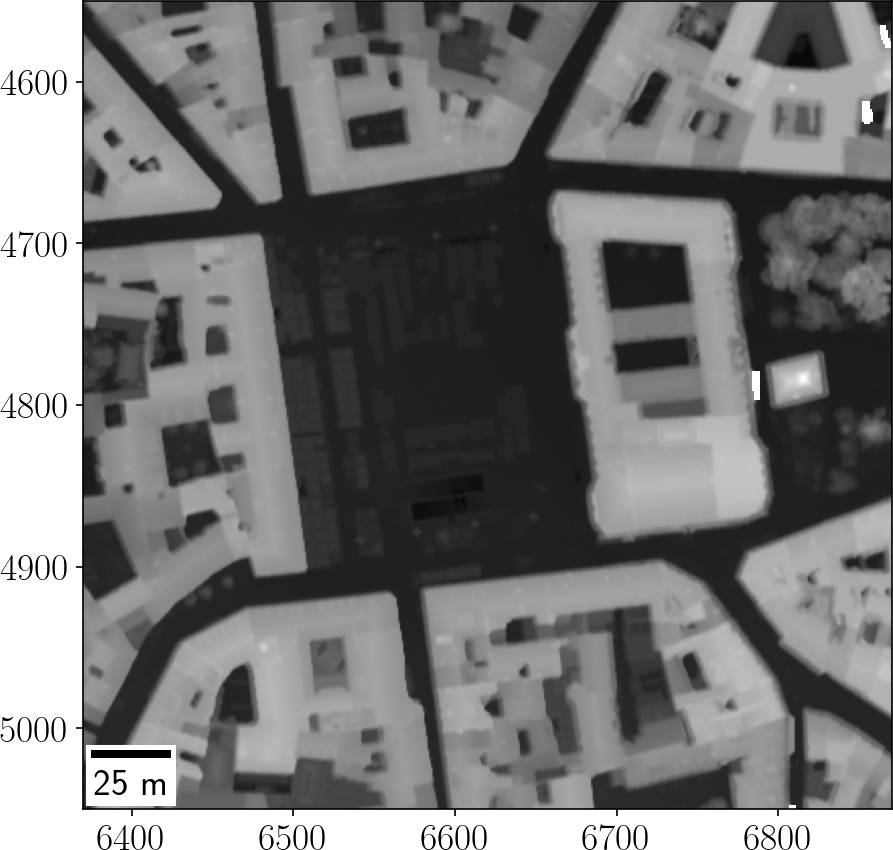
\includegraphics[height=6cm]{Images/Chap_1/DSM_Capitole_LiDAR.png}
        \caption{DSM from LiDAR HD data,\\Place du Capitole}
        \label{fig:DSM_capitole_lidar}
        %\begin{minipage}{.12cm}  % Multiline captions misalign figures
        %    \vfill              % This blank minipage is used to align
        %\end{minipage}          % images
    \end{subfigure}\hfill
    \begin{subfigure}[t]{0.5\linewidth}
        \centering
        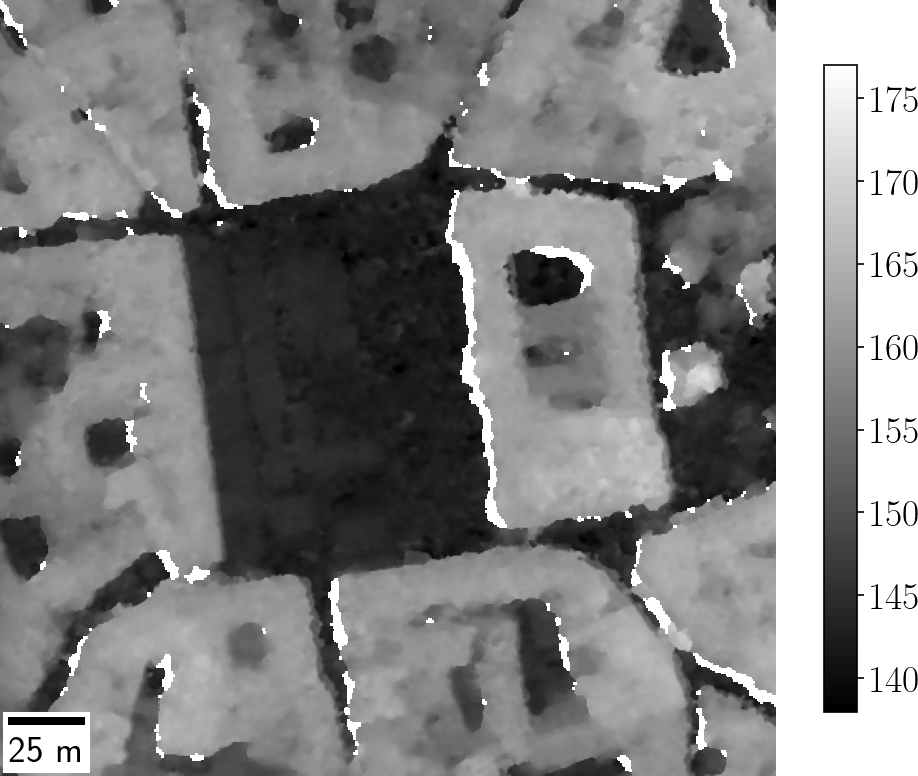
\includegraphics[height=6cm]{Images/Chap_1/DSM_Capitole_CARS.png}
        \caption{CARS DSM from Pléiades images,\\Place du Capitole}
        \label{fig:DSM_capitole_cars}
    \end{subfigure}
    \begin{subfigure}[t]{0.5\linewidth}
        \centering
        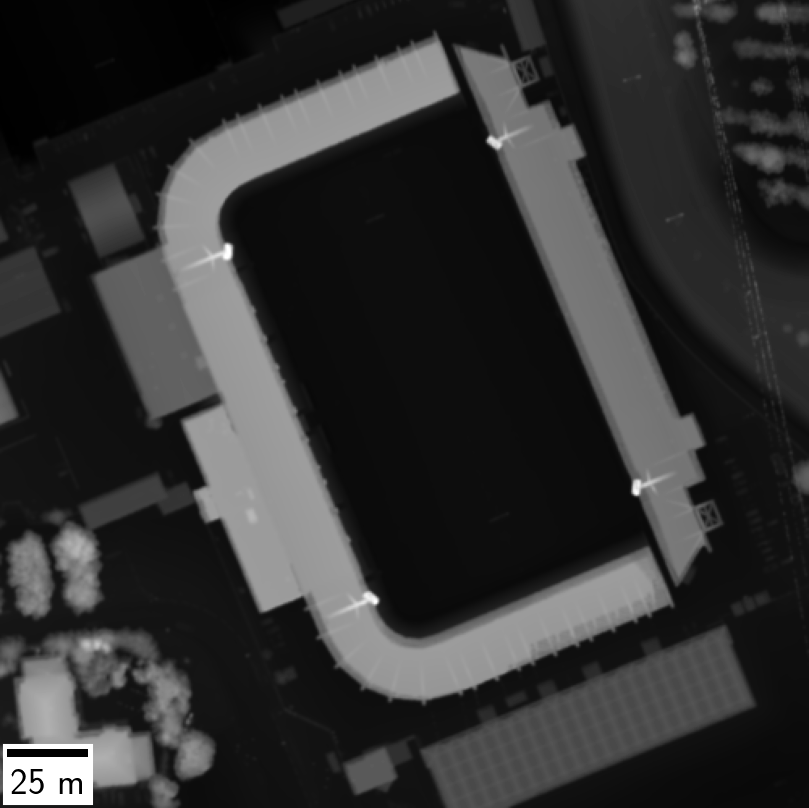
\includegraphics[height=6cm]{Images/Chap_1/DSM_Wallon_LiDAR.png}
        \caption{DSM from LiDAR HD data,\\Ernest Wallon stadium}
        \label{fig:DSM_ernest_wallon_lidar}
    \end{subfigure}\hfill
    \begin{subfigure}[t]{0.5\linewidth}
        \centering
        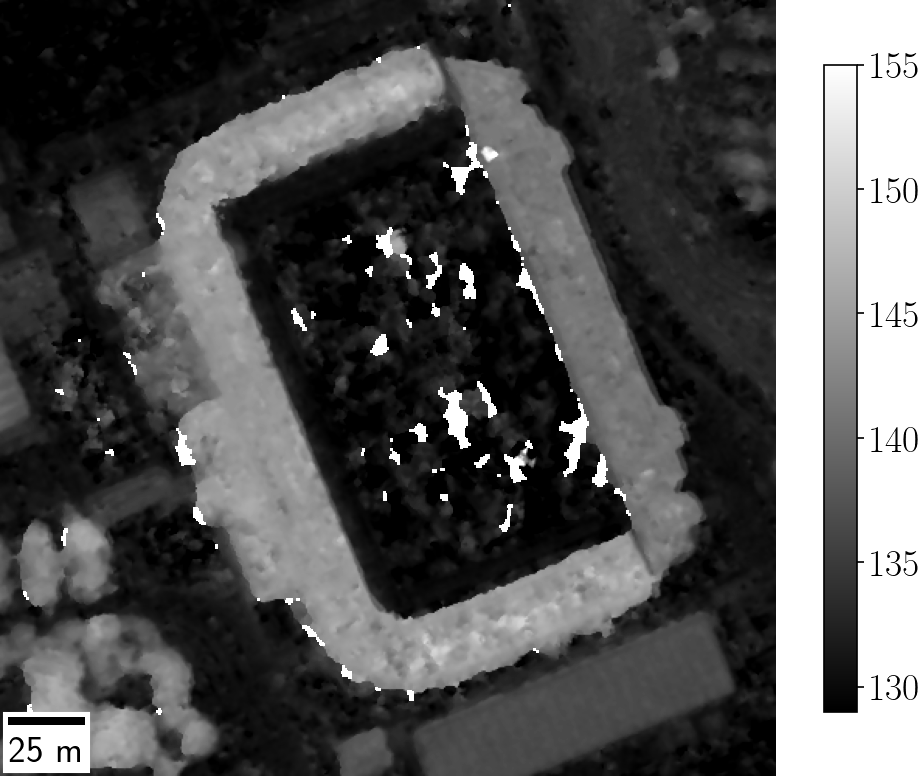
\includegraphics[height=6cm]{Images/Chap_1/DSM_Wallon_CARS.png}
        \caption{CARS DSM from Pléiades images,\\Ernest Wallon stadium}
        \label{fig:DSM_ernest_wallon_cars}
    \end{subfigure}
    \caption{Different DSM over Toulouse, France. DSM were obtained by rasterizing LiDAR HD data or by processing Pléiade stereo images with the CARS pipeline. The CARS pipeline uses a $5\times5$ CENSUS cost function and SGM regularization for stereo reconstruction. \copyright CNES 2017, Distribution AIRBUS DS}
    \label{fig:DSM_toulouse}
\end{figure}


Once the regularized cost volume $C_V^{SGM}$ has been computed, a simple \textit{winner-takes-all} strategy can be used to determine the disparity map $\mathcal{D}$:
\begin{align}
    \mathcal{D}(row, ~col) = \argmin_d C_V^{SGM}(row, col, d) 
\end{align}
\commanu{un peu court sur la stratégie de décision. rien à dire de plus sur l'état de l'art là dessus vu les échanges, et de perpectives? Peut etre juste une phrase du type: Winner takes all is the classical approach taken in literature but other approaches could be interesting to take especially with uncertainty information from this thesis.}

\subsubsection{Processing the Disparity Map}\label{sec:postprocess_disparity}
Once the disparity map has been computed, it is usually post-processed to remove artifacts, and improve disparity resolution.

It is common to add a sub-pixel refinement step, where a non-integer disparity is interpolated around the selected disparity. The main idea is to interpolate a model through the selected disparity $d=\argmin_\delta C_V(row, ~col, ~\delta)$ and its two direct neighbours\commanue{alors j'avais pas remarqué mais tu écris neighbors en anglais UK mais en général tu mets initialize donc c'est anglais US. Donc choisis ton côté de l'atlantique ;)}. The refined disparity $d_{interp}$ is then defined as the $\argmin$ of this interpolation model. \Cref{fig:sub-pixel_refinement} presents examples of interpolated disparities from  \cite{haller_real-time_2010}, mainly a ``V''-like shape as in \ref{fig:vfit_refinement} and a parabola as in \ref{fig:parabola_refinement}. Carrying out sub-pixel refinement suggests we assume the algorithm can attain a significant level of precision, which is debatable (see \Cref{sec:uncertainty_cars})\commanue{Et aussi que la fonction de coût a été suffisamment échantillonnée pour te permettre d'interpoler cotrrectement, ce qu'honnêtement on n'a jamais vérifié. On considère que c'est vrai}.\comloic{alors ça c'est très très inspiré d'autres outils comme s2p à dire vrai, et ce n'est pas forcément justifié. Enfin, disons qu'on utilise Census déjà, donc on peut oublier toute volonté d'étudier l'échantillonnage de la mesure à la capacité à reconstruire le signal correctement. Subpix = 2, = 4, = 48 compte tenu de la mesure Census on n'en sais rien donc on fait rien, et mieux, derrière on fait du V-fit. Là je crois que dans la littérature, s'il n'y a pas une explication il y a au moins une analyse empirique sur le choix de la méthode d'interpolation / approximation si on a utilisé du census}

\begin{figure}
    \centering
    \begin{subfigure}[t]{0.5\linewidth}
        \centering
        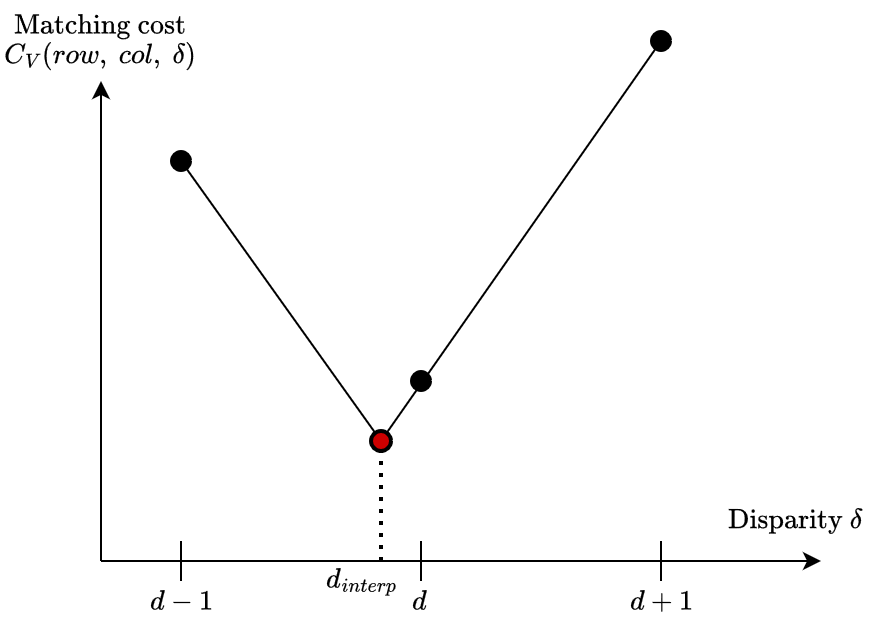
\includegraphics[width=\linewidth]{Images/Chap_1/subpixel_refinment_vfit.png}
        \caption{V-fit sub-pixel refinement}
        \label{fig:vfit_refinement}
    \end{subfigure}\hfill
    \begin{subfigure}[t]{0.5\linewidth}
        \centering
        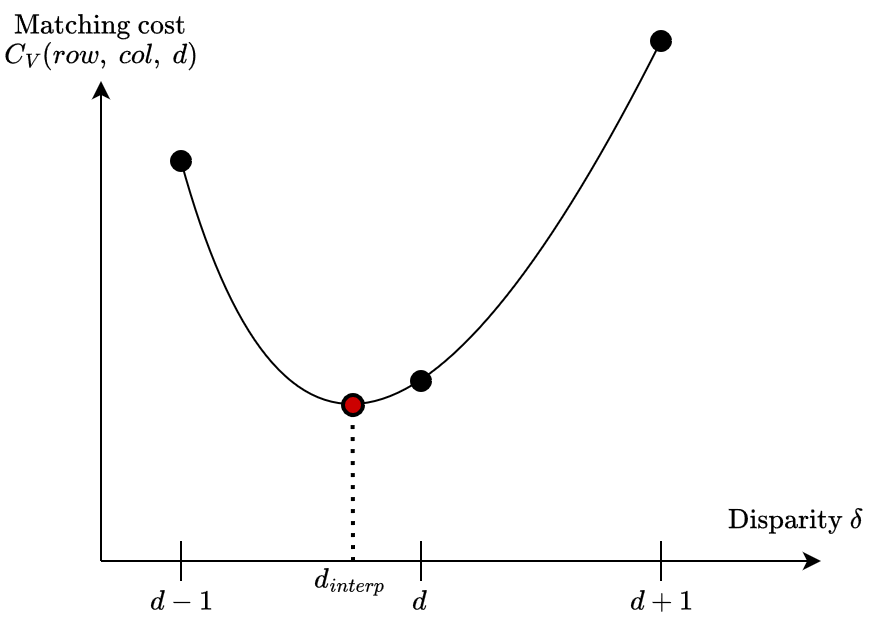
\includegraphics[width=\linewidth]{Images/Chap_1/subpixel_refinment_parabola.png}
        \caption{Parabola sub-pixel refinement}
        \label{fig:parabola_refinement}
    \end{subfigure}
    \caption{Different methods for refining the disparity $d=\argmin_\delta C_V(row, ~col, ~\delta)$}
    \label{fig:sub-pixel_refinement}
\end{figure}

The disparity map can also be filtered in order to remove local outliers. Classical strategies include the use of a mean or median filter for instance. There exists more advance filtering methods, such as bilateral filtering \cite{tomasi_bilateral_1998} which performs a weighted average, where weights depend on the proximity to other pixels both in the spatial and spectral domain. \comloic{en tout état de cause, tu peux argumenter que ton SGM fait déjà un filtrage de la carte de disparité dans la mesure où c'est WTA que tu enchaines derrière. Certains papiers oppose, voire meme compose, le filtrage bilatéral que tu cites, et SGM, lors d'une étape de régularisation du CV. }  

As presented previously, the \textit{winner-takes-all} strategy presents the inconvenient of allowing multiple pixels from the secondary image to be matched to the same pixel of the right image. For instance, if two pixels $(row,~col)$ and $(row,~col+1)$ from the second image have $d$ and $d-1$ as their respective disparity, they will be both matched to pixel $(row, ~col+d)$ in the reference image. This effect indicates that there is probably an error in the estimation of the disparity map. There exist strategies allowing to detect such error in order to eliminate dubious matches. A first strategy is called cross-checking\comloic{alors la validation croisée, elle peut faire ça, mais c'est pour ça qu'elle existe. D'ailleurs dans le scénario que tu cites, la validation croisée pourrait très bien ne pas rejeter aucun des deux matchs ((row, col)L, (row,col+d)R) et ((row,col+1)L, (row, col+d)R). Si tu pars de (row,col+d)R et que tu matchs ça avec (row,col+0,5)L puisque c'est sous pixellique, et que tu fais un seuil d'erreur à 1pixel, alors tu rejettes aucun des deux matchs précédents par la validation croisée. La validation croisée comme tu le montres avec la formule plus loin, c'est au niveau de D qui a été rafinée par interpolation sous pixellique. Ce que tu dis pourrais marcher si tu uilisais (row, col +2)L avec le tau=1 de l'équation 1.14. Dans tous les cas, en } \cite{fua_combining_1991}. We first start by computing a secondary cost volume $C_V'$ by reversing the roles of the images: the reference image becomes the secondary image and vice-versa. We then obtain two disparity maps $\mathcal{D}$ and $\mathcal{D}'$, and check that they are consistent, as in theory we would that $\mathcal{D}=-\mathcal{D}'$. A pixel $(row, ~col)$ is considered consistent across disparity maps if it verifies:
\begin{equation}\label{eq:cross-checking}
    |\mathcal{D}(row, col) + \mathcal{D}'(row, col+\mathcal{D}(row, col))|\leqslant \tau
\end{equation}
where $\tau$ is a consistency threshold usually set to $1$. For errors that do not check this consistency check, it has been proposed in \cite{hirschmuller_stereo_2008} to differentiate between mismatched pixels (pixels for which there exists a correct match) and occluded pixels (pixels that visible in an image but masked by an object in the other) as follows: if there is a disparity $d\in\mathcal{D}$ such that $\mathcal{D}'(row, col+d)=-d$ then it is a mismatch\commanue{la phrase est assez longue et en plus tu as des éléments en parenthèses. Il faudrait peut-être mieux splitter les éléments}. Otherwise, pixel $(row, ~col)$ is occluded. Occluded regions of an image can be filled by interpolation with the closest valid disparities\commanue{alors j'ai un doute on rebouche par interpolation avec les voisins les mismatch aussi, non?}.  

\begin{remark}
     \Cref{eq:cross-checking} requires the computation of a second cost volume, effectively doubles the processing time. As dense stereo matching is also the longest part of a photogrammetry pipeline, one might be reticent to carry out a cross-checking step. However, one might make the following observation: the cost volume contains the dissimilarity between every considered pair of pixels in the disparity range, so the cost of every considered match in the first cost volume is also present in the second cost volume. In theory, for every pixel $(row, ~col)$ and for every disparity $d$ in the (reference) disparity range, it holds \cite{bebis_mutual_2008}:
     \begin{align}\label{eq:diagonal_search}
         C_V(row,~col,~d) = C_V'(row,~col+d, -d)
     \end{align}
     \Cref{eq:diagonal_search} holds only for cost volumes obtained after the matching cost step. However, when SGM regularization or another aggregation cost method modifies cost volumes, then the there can be differences between $C_V(row,~col,~d)$ and $C_V'(row,~col+d, -d)$. In the case of SGM regularization, the differences between cost volumes are small and marginally modify the disparity maps. Using \eqref{eq:diagonal_search} then allow to obtain both cost volume by only computing one and re-indexing it to obtain the other. \todoroman{Ca c'est moi qui l'ait vérifié en faisant une batterie de tests https://confluence.cnes.fr/display/at3d/Faster+Right+Cost+Volume. J'ai pas trop de citations à fournir, est-ce que ça passe? Ou alors je le mets dans mes contributions.}\commanue{Tes contributions ce sont tes prez et articles. Là tu peux comme tu le mentionnes dire qu'après un ensemble de tests tu arrives à cette conclusion. Après Hirshmuller il se permet}
\end{remark}

\subsection{Triangulation}\label{sec:triangulation}
\commanu{une petite transition pour le lecteur, ca part direct sur le depth of a pixel sur une partie triangulation. rappelle peut etre l'objectif de la section et de l'étape métier.}
When working with pinhole camera models, the depth $z$ of a pixel is computed using the following formula:
\begin{equation}
	z=\frac{Bf}{d}\label{eq:z_bfd}
\end{equation}
where $B$ is the baseline between cameras, $f$ is the focal length of the camera, and $d$ is the disparity of a pixel. This formula can be found using optical geometry \cite{bolles_epipolar-plane_1987}, and illustrates the fact that pixels closer to the camera present a bigger position shift in between images\commanue{proposition mais vu comment les indiens ont corrigé mon doc je ne suis pas sure d'être une référence: pixels closer to the camera shift more significantly from one image to the other}. In the case of satellite imagery\commanue{Il me semble que tu l'as déjà dit donc j'ajouterais as mentioned previously au début de la phrase}, the pinhole camera model is not valid and we instead use other geometrical models\commanue{alors là ça fait traduction du français, je pense que sensor models est mieux} (see \Cref{sec:sensors_rpc}). \Cref{eq:z_bfd} thus cannot be used as such to provide accurate results.
\begin{remark}
    \Cref{eq:z_bfd}, although not used to determine the DSM, still provides an estimation of the height which can for instance used to determine the height of SIFT matches during the epipolar resampling step\commanue{C'est pas faux mais demandes-toi si il faut que tu gardes toutes les remarques. Je pense que celle-là tu peux supprimer}. \Cref{eq:z_bfd} also defines an important quantity, the $B/z$ ratio, usually called $B/H$ presented in \Cref{sec:epipolar_geometry}. This ratio is used to indicate the disposition of satellites\commanue{sensor positions} during the stereo acquisitions. A $B/H$ ratio near $0$ indicates a narrow angle between satellites\commanue{acquisitions car si tu n'as qu'un seul satellite...}, which will result in a DSM with few occluded areas but with low precision (an error of one disparity results in a larger height error)\commanue{Tu es comme Yannick un roi des parenthèses. Alors dans un manuscrit c'est pas un mail donc fait une autre phrase.}. Conversely, a higher $B/H$ ratio indicates a large angle between satellites\commanue{acquisitions}, resulting in a DSM with more occluded areas but with higher precision. In the case where one acquisition is made at nadir, the $B/H$ ratio equals the tangent of the angle formed between satellites views (see \Cref{fig:RPC}). For information purposes, the CO3D mission will provide acquisition with a $B/H$ ratio between $0.2$ and $0.3$.
\end{remark}

Instead, as RPC model\commanue{alors model c'est pour le verbe ou c'est RPC model le sujet et dans ce cas il te manque le verbe genre describe} every line of sight, we can use them to find the 3D coordinates of every match. To do so, first consider two stereo images, their RPC models $\RPC_1$, $\RPC_2$ from \cref{eq:rpc} as well as their epipolar grids $g_{e1}$, $g_{e2}$ from \cref{eq:epipolar_grid}. For every pixel $(row_e, ~col_e)$ from the reference epipolar image, whose disparity is $d$, then the 3D point $(X, Y, Z)$ represented by $(row, ~col)$ is the point verifying the following equations:
\begin{align}
    (X, Y, Z) &= \RPC^{-1}_1(g_{e_1}(row_e,~col_e),~Z)\label{eq:triangulation_exact}\\
    (X, Y, Z) &= \RPC^{-1}_2(g_{e_2}(row_e,~col_e+d),~Z) 
\end{align}
If the line\commanue{lines?} of sight intersect, then $Z$ is found by solving the following equation:
\begin{equation}
     \RPC^{-1}_1(g_{e_1}(row_e,~col_e),~Z) = \RPC^{-1}_2(g_{e_2}(row_e,~col_e+d),~Z) 
\end{equation}
Knowing $Z$ and $g_{e_1}(row_e,~col_e)$, \cref{eq:triangulation_exact} provides the $X$ and $Y$ coordinates as well.

\todoroman{En regardant le code de Shareloc, j'ai l'impression que chaque Line Of Sight est en fait une ligne droite lors de la triangulation. A verifier avec Manue/Manu/Loïc}\commanue{Alors je ne suis pas experte mais pour moi tu fais des segments car des RPC sont valides entre deux altitudes et ensuite tu cherches l'intersection ou le point le plus proche.}\commanu{dans shareloc, on a au départ un segment calculé sur  une alt min et alt max ou le RPC est valide mais transformé ensuite sur un starting point et viewing vector donc un point et un vecteur de direction donc une ligne pour la triangulation c'est bien ca qui est utilisé. donc ok avec description juste après, la référence de JMD est bien celle utilisé dans shareloc}
The problem is that lines of sight rarely present an exact intersection. By approximating line of sights by a starting point $P$, and a direction vector $\overrightarrow{V}$, we can instead define the coordinates $(X,Y,Z)$ as the point minimizing its distance two both lines. The exact formula for computing $(X,Y,Z)$ is provided in \cite{delvit_geometric_2006}:
\begin{equation}
    (X,Y,Z) = \left[ Id - V_1V_1^T + Id - V_2V_2^T \right]^{-1} \left[ (Id - V_1V_1^T)P_1 + (Id - V_2V_2^T)P_2 \right]
\end{equation}
where $Id$ is the identity matrix, and $V^T$ is the transposed vector $V$.

Triangulating every point using the disparity map leads to a 3D point cloud. Because we know from which pixel each 3D point originates from, we can associate to every 3D point additional information such as:
\begin{itemize}
    \item The color of the reference pixel (if provided). The point cloud is thus a colored point cloud.
    \item Confidence measures computed during the dense-matching step\commanue{Oui c'est vrai mais tu n'as jamais mentionné les mesures de confiance}. 
\end{itemize}

The 3D points can be filtered to remove obvious errors. Two different filtering\commanu{c'est quand meme bizarre de garder triangulation et filtrage dans la meme section. Si tu parles de filtrage (est ce utile ?), fais une sous section, je pense} steps are carried out: one for removing statistical outliers, and one for removing so-called ``small-components''\commanue{Alors ça c'est les filtrages de CARS}. 
\subsubsection{Statistical outliers filtering}
Points that are statistical outliers, are determined by considering the positions of its neighbours. For each point $P$, we compute the mean distance $\mu_P$ to its $N$ neighbours. Then we can compute for each point $P$ the mean distance $\mu$ and standard deviation $\sigma$ of its $N$ neighbours as:
\begin{align}
    \mu &= \frac{1}{N}\sum_{i=1}^N\mu_i\\
    \sigma &= \sqrt{\frac{1}{N-1}\sum_{i=1}^N(\mu_i-\mu)^2}
\end{align}

A point $P$ is considered to be a statistical outlier if its mean distance $\mu_P$ its far away from the mean distance of all of its neighbours according to the following criterion:
\begin{align}
    \mu_P>\mu+k\sigma
\end{align}
Where $k$ is a constant set by the user, usually set to $5$. We also consider $N=50$.

\subsubsection{Small-components filtering}
The other filtering method, named small-components filtering, attempts to remove small isolated clusters of points. For each point, we count the number of neighbours $N$ present within a distance $D_{max}$. If this number is inferior to a given threshold $N_{min}$, then we consider the point belongs to a small component and is removed. Formally, a point $P$ is removed if:
\begin{align}
    \#\{~\text{Points } Q~|~\sqrt{(P-Q)(P-Q)^T}\leqslant D_{max}~\}\leqslant N_{min}
\end{align}
We usually set $D_{max}$ to $3m$ and $N_{min}$ to $50$.

\Cref{fig:point_cloud_filtering} illustrates the two filtering methods presented. More advanced filtering methods can be implemented, such as bilateral filtering \cite{digne_bilateral_2017}, and filtering using color information or confidence measures from the disparity map (see \Cref{sec:uncertainty_pandora}) \cite{youssefi_geometrically_2024}\commanue{je mettrais ce paragraphe plus haut quand tu mentionnes les filtres de CARS et avant de les décrire en détail}.

\begin{figure}
    \centering
    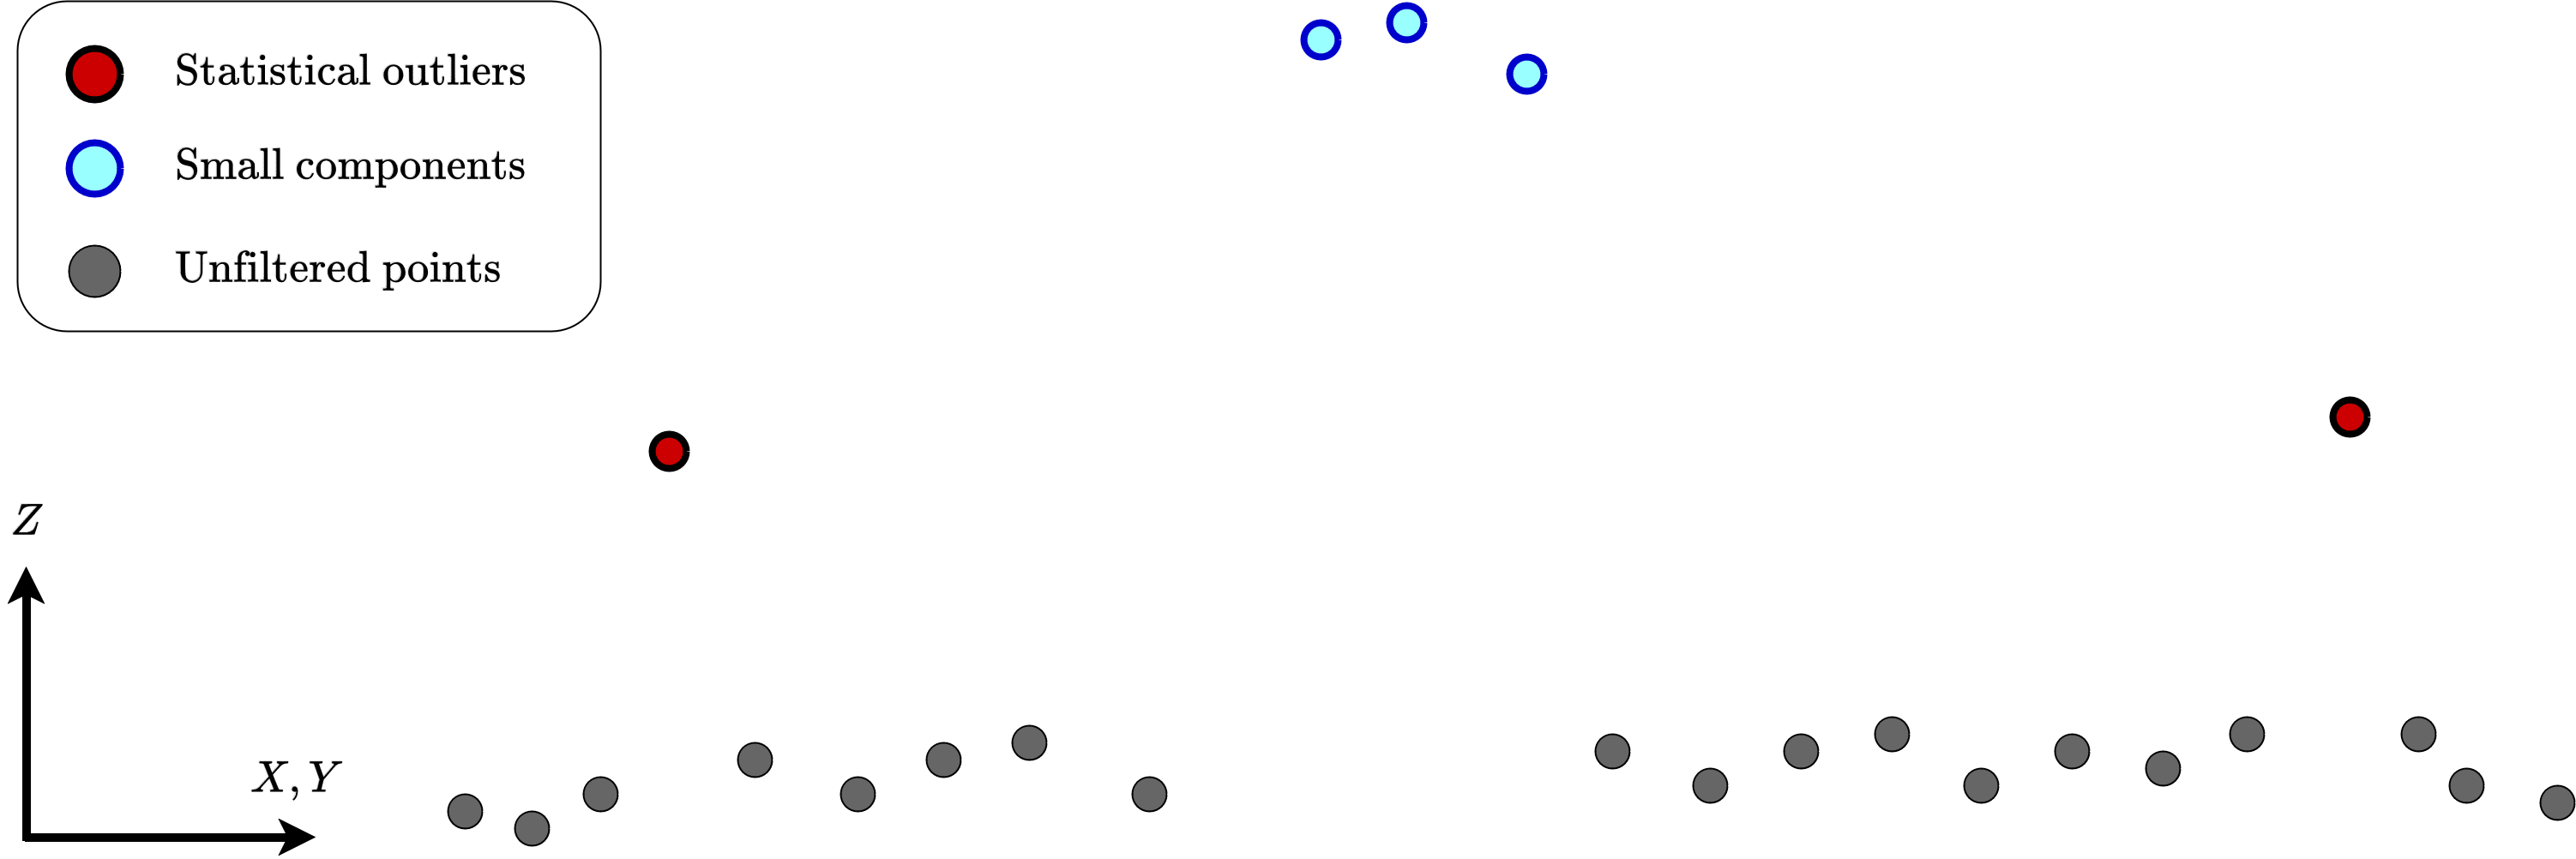
\includegraphics[width=\linewidth]{Images/Chap_1/Point_cloud_filtering.png}
    \caption{Example of statistical outliers and small components filtering of a 3D point cloud.}
    \label{fig:point_cloud_filtering}
\end{figure}

Filtering the point cloud results in a 3D product that can already be provided as such to users. However, point clouds, while containing more 3D information than DSM, can be hard to manipulate in conjunction with other \acrshort{gis} data. Projecting the point cloud on a regular grid to produce a DSM is thus often preferred, which constitutes the final step of the stereo pipeline.

\subsection{Rasterization}\label{sec:rasterization}
Rasterization consists in projecting the 3D points onto a regular grid over the $(X,Y$) plane to produce the final DSM. One of the challenges faced when projecting the point cloud is that of the relative\commanue{low?} density of the point cloud relative to the DSM grid. Indeed, if the density of the point cloud is high enough, multiple 3D points can be projected to the same cell, which raises the question on how to merge their 3D information. On the other hand, if the density is low enough\commanue{loo low?}, there may some cells where no points are projected onto. 

The CARS stereo pipeline uses a Gaussian interpolation to fuse the information of point clouds. Given a cell with coordinates $(X,Y)$ of the DSM, we consider every point $P_i=(X_i, Y_i, Z_i)$ in a given radius $r$ of $(X,Y)$, and note $\mathcal{N}_{XY}$ the set of all those points. The final value of the DSM is then computed as the following mean with Gaussian weights:
\begin{align}
    \DSM(X,Y) &= \frac{\sum_{P_i\in\mathcal{N}_{XY}}Z_i\cdot e^{-\frac{(X_i-X)^2+(Y_i-Y)^2}{2\sigma^2}}}{\sum_{P_i\in\mathcal{N}_{XY}} e^{-\frac{(X_i-X)^2+(Y_i-Y)^2}{2\sigma^2}}}
\end{align}
with sigma usually set to $0.3m$ and the radius $r$ being $3m$. \Cref{fig:rasterization} illustrates the rasterization process.

Rasterizing with this method presents\commanue{provides/offers pour éviter la répétition de present} the advantage of smoothing the potential height variations still present in the 3D point cloud, while allocating more weight to points that are near the cell center. This method can also be found in other stereo pipelines \cite{shean_automated_2016}, while other pipelines use different weighting methods, such as Inverse Distance Weightings (IDW) \cite{rupnik_micmac_2017}, producing similar results.

\begin{figure}
    \centering
    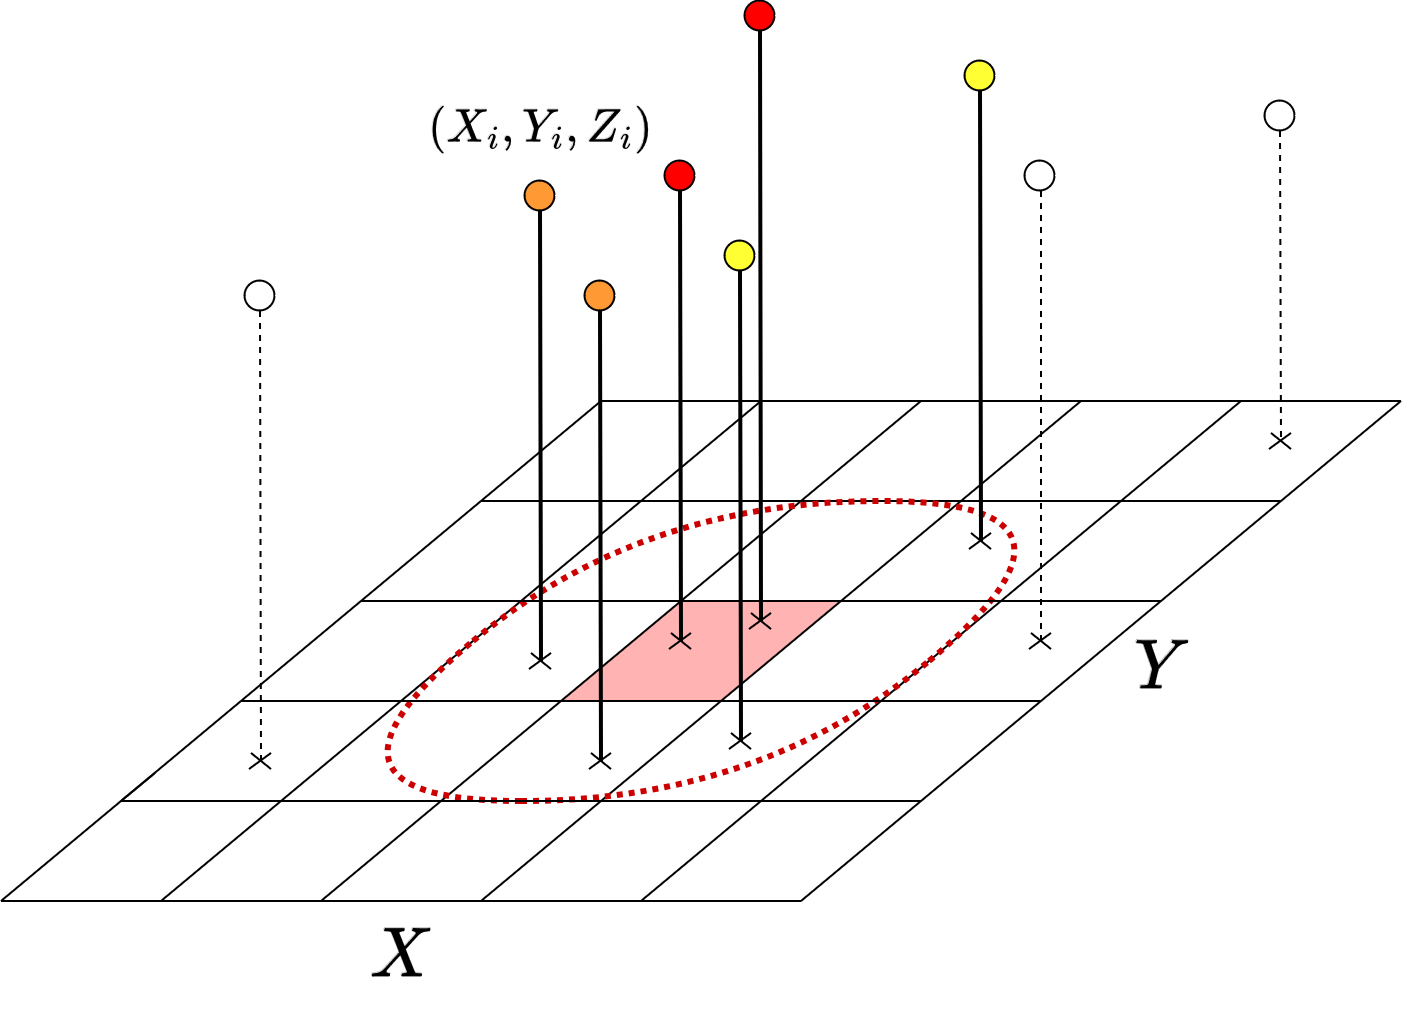
\includegraphics[width=0.7\linewidth]{Images/Chap_1/Rasterization.png}
    \caption{Rasterization of the point clouds on a regular grid. Red points are nearer to the center $(X,Y)$ of the considered cell, while yellow points are further away.}
    \label{fig:rasterization}
\end{figure}

\begin{remark}
    If no points are projected in a given cell (or its direct neighbours), then the cell can be filled with \textit{nodata} values. Different method can be considered to fill holes, such as directly using the values of nearest valid neighbouring cells, or interpolating their values. More advanced methods consists in simulating a cloth-like surface fill the holes as in \cite{lallement_bulldozer_2022}.
\end{remark}

\subsection{From LiDAR to Ground Truth Disparity}
\commanu{bizarre dans la section stereophotogrammetry pipeline. C'est plus pour la qualification. T'as vraiment besoin d'expliquer ou tu peux juste citer dans ta partie résultats quand tu abordes la qualification ? tu verras si ca saute pas du coup. Moi j'enleverais d'ici, ca n'a pas vraiment sa place, je trouve}
Parler du LiDAR HD en général. 

Explaination on how to obtain GT disparity maps from georeferenced LiDAR, \cite{cournet_ground_2020}. Line of sight and default geoid. 

\section{Uncertainty in Stereophotogrammetry}\label{sec:previous_work_stereo_uncertainty}
\todoroman{Sources d'incertitudes : acquisition des images et bruit sur le capteur. Précision du model RPC. Incertitude issue des différentes traitement (rééchantillonage, stereo matching). Intersection des lignes de visée. Rasterization.}
\commanu{du coup intro de la section à faire pour comprendre le déroulé ensuite}
\commanu{bien mettre en avant quelque part début ou fin de la section qu'il y a peu de travaux sur le sujet et que donc ton travail est novateur et défriche quelque chose de peu regardé. Remarque des implémenteurs de Mic Mac: c'est trop complexe. donc mettre quelque chose qui donne ce recul au lecteur et qui explique qu'il n'y ait pas bcp de travaux cités. Ce n'est pas un raté de ton travail d'état du lard!}
\subsection{Previous work}
\commanu{titre: on dirait que c'est ton travail précédent. Plutot state of the art?}
\todoroman{Regarder ce qui se fait sur les autres produits 3D: BD ALTI \url{https://geoservices.ign.fr/bdalti}, section 2.2.2 \url{https://geoservices.ign.fr/sites/default/files/2021-07/DC_RGEALTI_2-0.pdf}. Mission Copenicus avec WorldDEM par TandDEM X \url{https://fr.wikipedia.org/wiki/TanDEM-X}}

The quality of \acrshort{dsm} obtained using stereophotogrammetry can greatly vary depending on the quality/resolution of the images used, the precision of the geolocation, the performances of the stereo matching algorithm \etc. Reducing the magnitude of errors, or evaluating the uncertainty \textit{a posteriori} has been investigated in multiple work.
Uncertainty on \acrshort{dsm} has been mainly evaluate using a single confidence interval over the whole DSM \cite{hugonnet_uncertainty_2022, deschamps-berger_apport_2021, wang_robust_2015, oksanen_digital_2006,panagiotakis_validation_2018}. Intervals are computed based on a set of reference points, either extracted from a better resolution \acrshort{dsm}, or ground truth data. \todoroman{Reprendre le papier où ils samplent depuis leur prorpre DSM}. Fusing \acrshort{dsm} to get better accuracy \cite{qin_uncertainty-guided_2022}
\cite{hu_quantitative_2012,poggi_confidence_2021}
Deep uncertainty for disparity?

The ASP pipeline\commanu{je remettrais: The NASA's ASP pipeline cited before... } can take as inputs camera standard deviation of position uncertainty (expressed in meters) in the horizontal ground plane, and propagate it during the triangulation and rasterization steps. The documentation (\url{https://stereopipeline.readthedocs.io/en/stable/error_propagation.html}) details the covariance matrix propagation method used. It explicitly states that the propagated uncertainty does not represent the error between the predicted height and a hypothetical ground truth, even though they are expressed in the same unit of measure. It is rather the propagated covariance from the camera position projected in the horizontal and vertical directions, regardless of the matching errors or triangulation error if the line of sight do not intersect.

\subsection{Uncertainty in the CARS pipeline}\label{sec:uncertainty_cars}
In this thesis, we focused on quantifying the uncertainty alongside the creation process of \acrshort{dsm}. We thus differ in this regard from previous work, which produces a single confidence intervals from the final produced DSM. Multiple sources of uncertainty influence the production of a DSM, which we will now detail\commanu{proposition: I will now detail the multiple sources of uncertainty that influence the DSM production. remarque tjrs sur I et we, choisis et sois cohérent sur l'ensemble}.

First, the images contain noise from the captor\commanue{sensor?}, and some atmospheric effects may appear on the acquisitions. For push-broom sensors, satellite movements can have a big impact on the final images. For instance, vibration of the satellite that are not taken into account in the geometric model can lead to biases on the geolocation of the different rows of the image. Those biases will themselves be propagated to the final DSM. Those are the main uncertainties associated with the input data.\commanu{en gros tu aurais des effets sur la radiométrie (pas forcément que le bruit et l'atmosphère, ca peut etre compression ou autre artefact dans la production, je suis pas expert mais quasi sur que plein de choses...) et la géométrie (pas forcément que les vibrations, ca peut etre un mauvais calage, une mauvaise référence, je dirais qu'il y a plus que les vibrations, voir daniel). Bref, tu dois pouvoir généraliser en "radiométrie" et "géométrie" pour etre plus juste, tout en citant en exemple ce que tu as mis. A mon avis, l'analyse d'incertitude sur ces "input data" pourrait etre une thèse en soi, donc un peu court}

Other errors occur when processing this data. First, different resampling\commanue{several resamplings?} occur in order to convert stereo images from captor\commanue{alors captor je ne suis pas fan je mettrais sensor} geometry to epipolar geometry. Those resamplings introduce errors if the input and target resolutions do not respect Shannon criteria \cite{delon_small_2007} \todoroman{mettre les formules? affiner la phrase}. Moreover, the sparse matches used to refine the epipolar grid heavily\commanue{strongly?} depend on the performance of the SIFT algorithm used to obtain them. In similar terrain, for instance on glaciers where many homogeneous region are present, some false matches can be observed. This leads to wrong epipolar lines, and those errors will themselves be propagated in the following steps of the pipeline\commanue{Oui on a aussi un problème sur des champs où l'alignement n'était pas bon. Après je pense que c'est surtout qu'avec les SIFTS parfois on trouve pas le bon intervalle...}. Those errors are usually minor, compared to those occurring in the dense stereo matching step\commanue{Ah bah voilà c'est forcément la faute de pandora. David et Dimitri ont trop déteint sur toi ;)}.

Dense stereo matching is a complex task, for which many different algorithms exist, each potentially presenting different performances. Using a window-based correlator with SGM regularization usually presents good performance in areas without height discontinuities. This can become a problem in urban areas, where the presence of high buildings represents an additional challenge for the correlator. Because the correlator compares windows ($5\times5$ using the CENSUS cost function or $11\times11$ using MC-CNN) and not single pixels, this naturally creates an adherence effect near building borders\commanue{Alors moi j'ai lu les différentes versions de ce chapitre donc là il faut peur-être faire un renvoi à l'adhérence}. Note that in \cite{okutomi_stereo_1994}, authors have been trying to adapt the window shape to reduce the uncertainty of stereo matching, but this method requires to iteratively compute costs on different windows, which can become quite expensive. SGM regularization also penalizes disparity changes, thus reinforcing the adherence effect. Other processes, such as filtering or sub-pixel refinement, improve the quality of the disparity map but require specific care for handling their induced uncertainty. Sub-pixel refinement also supposes that sub-pixel disparities can be deducted without upsampling the input images, which is debatable\commanue{C'est plutôt qu'on ne vérifie pas que la fonction de coût est suffismament échantillonnée et effectivement si ce n'était pas le cas il faudrait suréchantillonner l'image, là tu me fais un peu la version raccourcie}. The dense matching step is crucial as previous errors usually have a smaller impact on the final product than the errors potentially occurring in stereo-matching\commanue{Même si la phrase me rend triste il faudrait la mettre en début du paragraphe, elle est importante et te fera le lien avec avant. D'ailleurs tu peux mettre aussi le reste du paragraphe avant.}. For instance, a bias in the epipolar grid typically leads to a shift of one row between the epipolar images. This leads to typical errors of around $1$ disparity. In comparison, the correlator can produce errors with a magnitude of the whole disparity research interval, sometimes reaching values near $100$ disparities. Considering those orders of magnitude, estimating and quantifying the uncertainty of the stereo-matching process is crucial to control the uncertainty on the output DSM. \Cref{sec:uncertainty_pandora} dives more into details regarding the different methods that have been developed to quantify the uncertainty of dense stereo matching.

Once the disparity has been estimated, 3D points can be triangulated by intersecting RPC lines from each matched pixel. However, we saw previously that there is no guarantee that the 3D lines do intersect. If they indeed do not intersect, the 3D point is defined as the point minimizing its squared distances to both lines of sight. An alternative is to modify the geolocation line from the secondary image so as it intersects the line from the reference image. In both cases, the localization of the 3D point is not exact. This uncertainty stems from the fact that we determine the 3D coordinates of the point from a match between two pixels that do not point exactly to the same object\commanue{Je comprends ce que tu veux dire mais il faudrait voir si on peut pas améliorer la formulation. Avec l'échantillonnage des pixels les pixels ne sont pas exactement comparable. Je réfléchis à comment le reformuler}. Additionally, RPC models attempt to represent real lines of sight with polynomial coefficient, which is not exact and possess its own accuracy. The method used for coefficients calibration and the frequency of calibration also bring their share of uncertainty.

The final part of the stereo pipeline is to rasterize the point cloud onto a regular grid, thus yielding the DSM. When characterizing the uncertainty on the final result, we must first agree on what the DSM is supposed to represent. It is common to consider that each pixel's value should represent the average height over the cell. However, providing the maximum or minimal height might be more adapted to some scenarios: for instance if the DSM is used to prepare very low altitude flights (for drones \etc), the maximum height is more relevant as one would want to avoid any foliage or power line. Those elements could disappear in the fin\commanue{clairement il manque la fin ;)}. In this thesis, we will consider that the DSM represents the (weighted) average height. The weights considered will be computed with a Gaussian whose variable is the distance to the center of the cell\commanue{Remarque un peu globale mise à l'arrache ici, mais il faudrait relire quand tu auras fini la partie d'avant pour voir si ça ne fait pas trop redite avec la description du pipeline}. Other weights can be considered, most notably the \textit{inverse distance weighting} (IDW), which produces very similar results in our applications. We now specified the projection method\commanue{Pourquoi au passé?}. Depending of the resolution of input images and the desired output resolution of the DSM, the density of points per DSM cell will vary. In our applications, the input and output resolutions are identical as we typically desire to produce a DSM at $50$cm resolution from $50$cm panchromatic images. This means that there is on average one 3D point per DSM cell. For occluded regions, or when we discarded stereo matches that seemed wrong, there might be no point directly in the output cell. In this case, the value of the DSM cell will be completely determined by the value of points in neighbouring cells, even if their distance is high and the averaging weights are small. Interpreting the final DSM as the average height on each cell is thus debatable, as the average is computed on a limited number of points, and sometimes not even belonging to the considered cell.  Note that if there is no points around in a given radius, the cell will be left empty. 

Different sources of uncertainty occurring throughout the stereo pipeline were presented in the previous paragraphs. Characterizing, modelling and propagating all of those uncertainties could not be considered in the span of this thesis. We thus focus mostly on the uncertainty arising from the dense stereo matching step, as it is the source of the biggest errors in the pipeline. \Cref{chap:propagating} investigates how uncertainty from the input epipolar images can be propagated in the stereo matching step, and \Cref{chap:epistemic_uncertainty} attempts to model the processing uncertainty of stereo algorithm itself. We also propagate this uncertainty all the way to the output DSM and show that it can correctly estimate the errors made during the DSM production. 

We conclude this section with a small disclaimer: our methodology estimates the uncertainty independently for every pixels, leading to small confidence intervals in confident areas, and bigger confidence intervals where the algorithms may have performed badly. We differ in this regard to the methods presented in \Cref{sec:previous_work_stereo_uncertainty}, which estimate a single global confidence interval \textit{a posteriori}, based solely on the DSM (and reference points), regardless of the method used to obtain it. In this regard, it does not seem relevant to compare our intervals to theirs, as there most similar characteristics is their name ``interval'', but neither share the same form (single \vs multiple intervals), nor are based on the same data. \commanu{je me demande si tu peux pas mettre cette dernière partie dans une sous section à part. Ce ne serait donc pas un disclaimer mais une présentation  Cette sous section (et la suivante sur le dense matching) décrit les sources d'incertitude que tu vois et pourrait amener à une sous section de transition ou tu expliques et justifies les choix pris pour la thèse vers le chap 4 et 5 en disant que l'idée était de prendre aussi les techniques méthodologiques du chap 2 et 3 en considération. }

\subsection{Uncertainty Quantification in Dense Stereo Matching}\label{sec:uncertainty_pandora}
As stereo-matching is a popular problem in computer vision, many methods for quantifying its uncertainty have been proposed in the literature. Without being exhaustive, this section presents a quick overview of the main approaches as well as the solutions currently implemented in the dense stereo correlator Pandora used in the CARS pipeline.

The way uncertainty is quantified in stereo matching is by producing \textit{confidence maps}, \ie a mapping for each pixel $(row, ~col)$ to a real confidence value, usually between $0$ and $1$. By convention, a value of $0$ means that we are not confident in the disparity value associated to $(row, ~col)$. Conversely, a confidence value of $1$ indicates that we are very confidence in the predicted disparity.

\begin{remark}
    \todoroman{Faire relire cette remarque à Manue et Seb car je l'ai écrite après leur relecture }It is interesting to see that in \cite{quinio_random_1992}, the author considered using closed random sets (a concept related to imprecise probabilities and belief functions studied in \cref{chap:representation_of_uncertainty} \cite{quinio_random_1991}) to model the uncertainty of a stereoscopic setup. They mainly consider the uncertainty arsing from the limited resolution of digital images (as we do in \cref{chap:propagating}), and from the precision of the calibration setup: focal length of cameras, baseline distance, orientation and vengeance angle of the cameras \etc. They consider that the uncertainty from dense matching is not of epistemic nature, but of aleatoric nature, and thus do not model it by imprecise models as we do in \Cref{chap:epistemic_uncertainty}. This hypothesis is justified as they achieve the stereo matching step using a window based ZNCC cost function (without \acrshort{sgm}, as it was not published at the time), which by nature possess strong links with probabilistic models.
\end{remark}

There are multiple sources of information that can be used to compute a confidence measure. Left and right input images and the predicted disparity map being those available to every method, but cost-based approaches can also make use of the cost volume, as it contains a lot of useful information. Most confidence measures were first handcrafted using those different information sources. For reviews on those methods, we refer to \cite{egnal_stereo_2004, hu_quantitative_2012, poggi_quantitative_2017}. With the rising use of deep-learning in stereo, many networks have been developed to estimate the uncertainty. A review for methods using regression forests can be found in \cite{min-gyu_park_leveraging_2015}, and a more general review, including the use 2D and 3D CNNs on the cost volume, can be found in \cite{poggi_confidence_2021}.

\begin{remark}
     Quantifying the uncertainty in stereo matching is a popular field of research. Recently, people have even been trying to evaluate the uncertainty of the confidence estimation itself, called \textit{meta-confidence} \cite{kim_meta-confidence_2022}.
\end{remark}

\begin{example}
    Let us present some examples of confidence measures that use different sources of information.\commanue{Pourquoi tu ne mets pas cette phrase à l'extérieur de l'encart, afin de ne pas avoir l'encart qui poppe. Après je ne sais pas au final si un encart est nécessaire.}
    
    Regarding confidence measure based on the disparity map, we already presented a type of binary confidence measure in \Cref{sec:postprocess_disparity} with the cross-checking test from \cref{eq:cross-checking}. Other methods compute for instance the local variance of the disparity map, where a low variance suggests confident regions.
    
    For methods using the cost volume, a simple method for measuring the cost would be using the value of the matching score measure (MSM, \cite{egnal_stereo_2004}) for a given disparity at coordinates $(row, ~col)$:
    \begin{equation}
        MSM(row, ~col) = -C_V(row, col, \mathcal{D}(row, ~col))
    \end{equation}
    This measure can be normalized between $0$ and $1$ using the global minimum and maximum of the cost volume. The idea behind this measure is the following: a high matching cost for a selected disparity indicates that the two matched pixels are not that similar, and thus the match is not confident. Other measures using the matching cost compare the value of the first and second minimum of a cost curve, or measure the curvature of the cost curves. More advances measures make use of 3D CNNs on the entirety of the cost volume to learn an efficient confidence measure \cite{mehltretter_cnn-based_2019}.
    
    Measures based on the input images usually measure the gradient \cite{haeusler_ensemble_2013} or variance \cite{park_learning_2019} of input images. High gradient or high variances indicate highly-textured regions, which are often easier to match. The confidence is therefore higher for those pixels. 
    
    Deep-learning approaches can combine multiple sources of information (input images, cost volume, disparity map) to learn a confidence measure \cite{tosi_beyond_2018, kim_adversarial_2020}.
\end{example}

In this thesis, we will also consider three confidence measures that can already be computed with our correlator. Those measures will help us to quantify the uncertainty in the photogrammetry pipeline or will be used as comparison with our proposed method.

\begin{figure}
    \centering
    \begin{subfigure}[t]{0.5\linewidth}
        \centering
        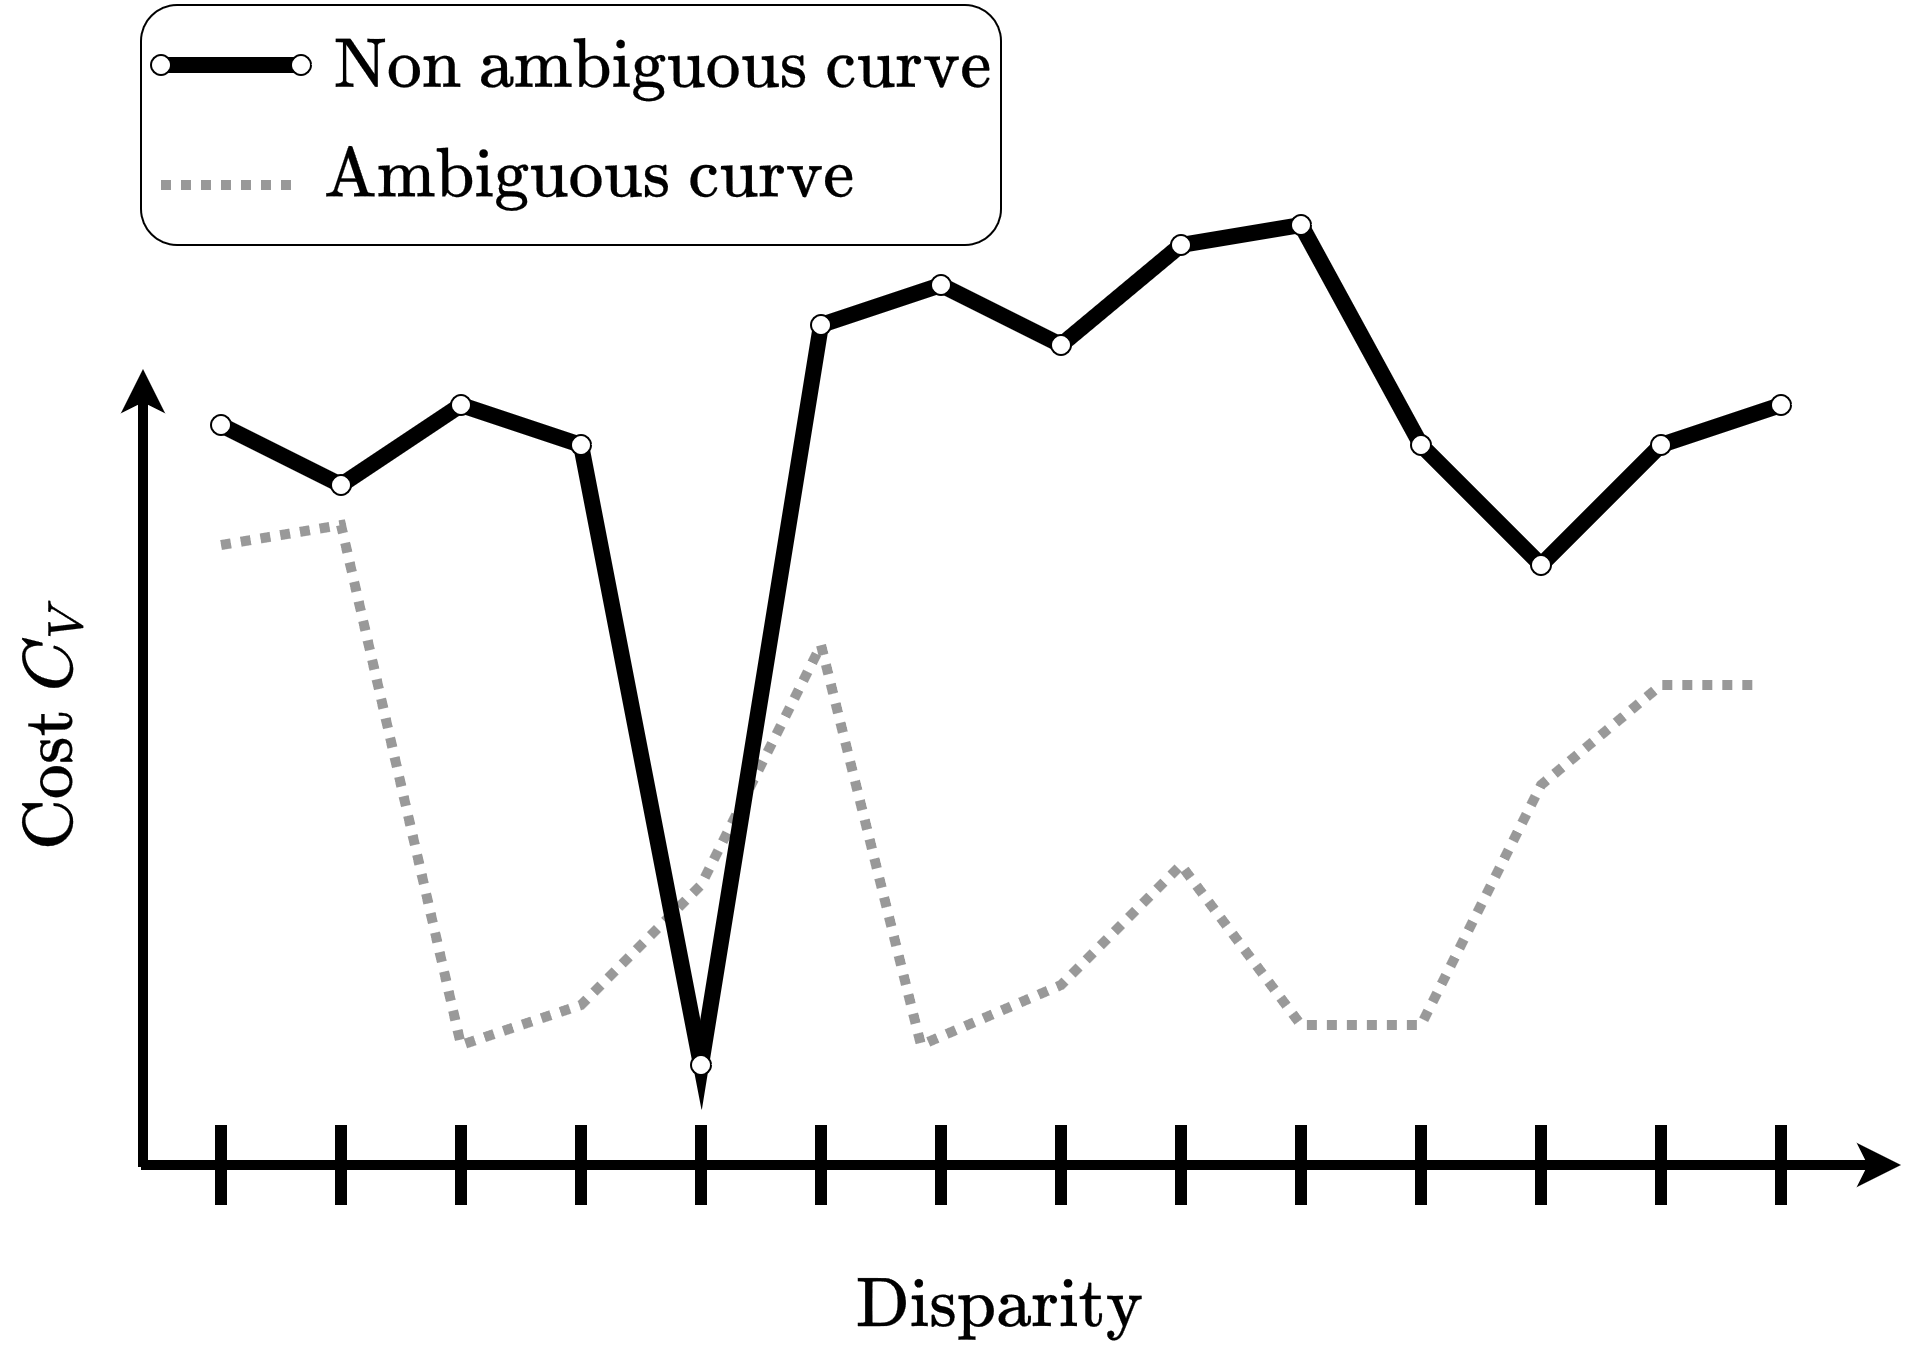
\includegraphics[width=\linewidth]{Images/Chap_1/Ambiguity.png}
        \caption{}
        \label{fig:ambgiuity}
    \end{subfigure}\hfill
    \begin{subfigure}[t]{0.5\linewidth}
        \centering
        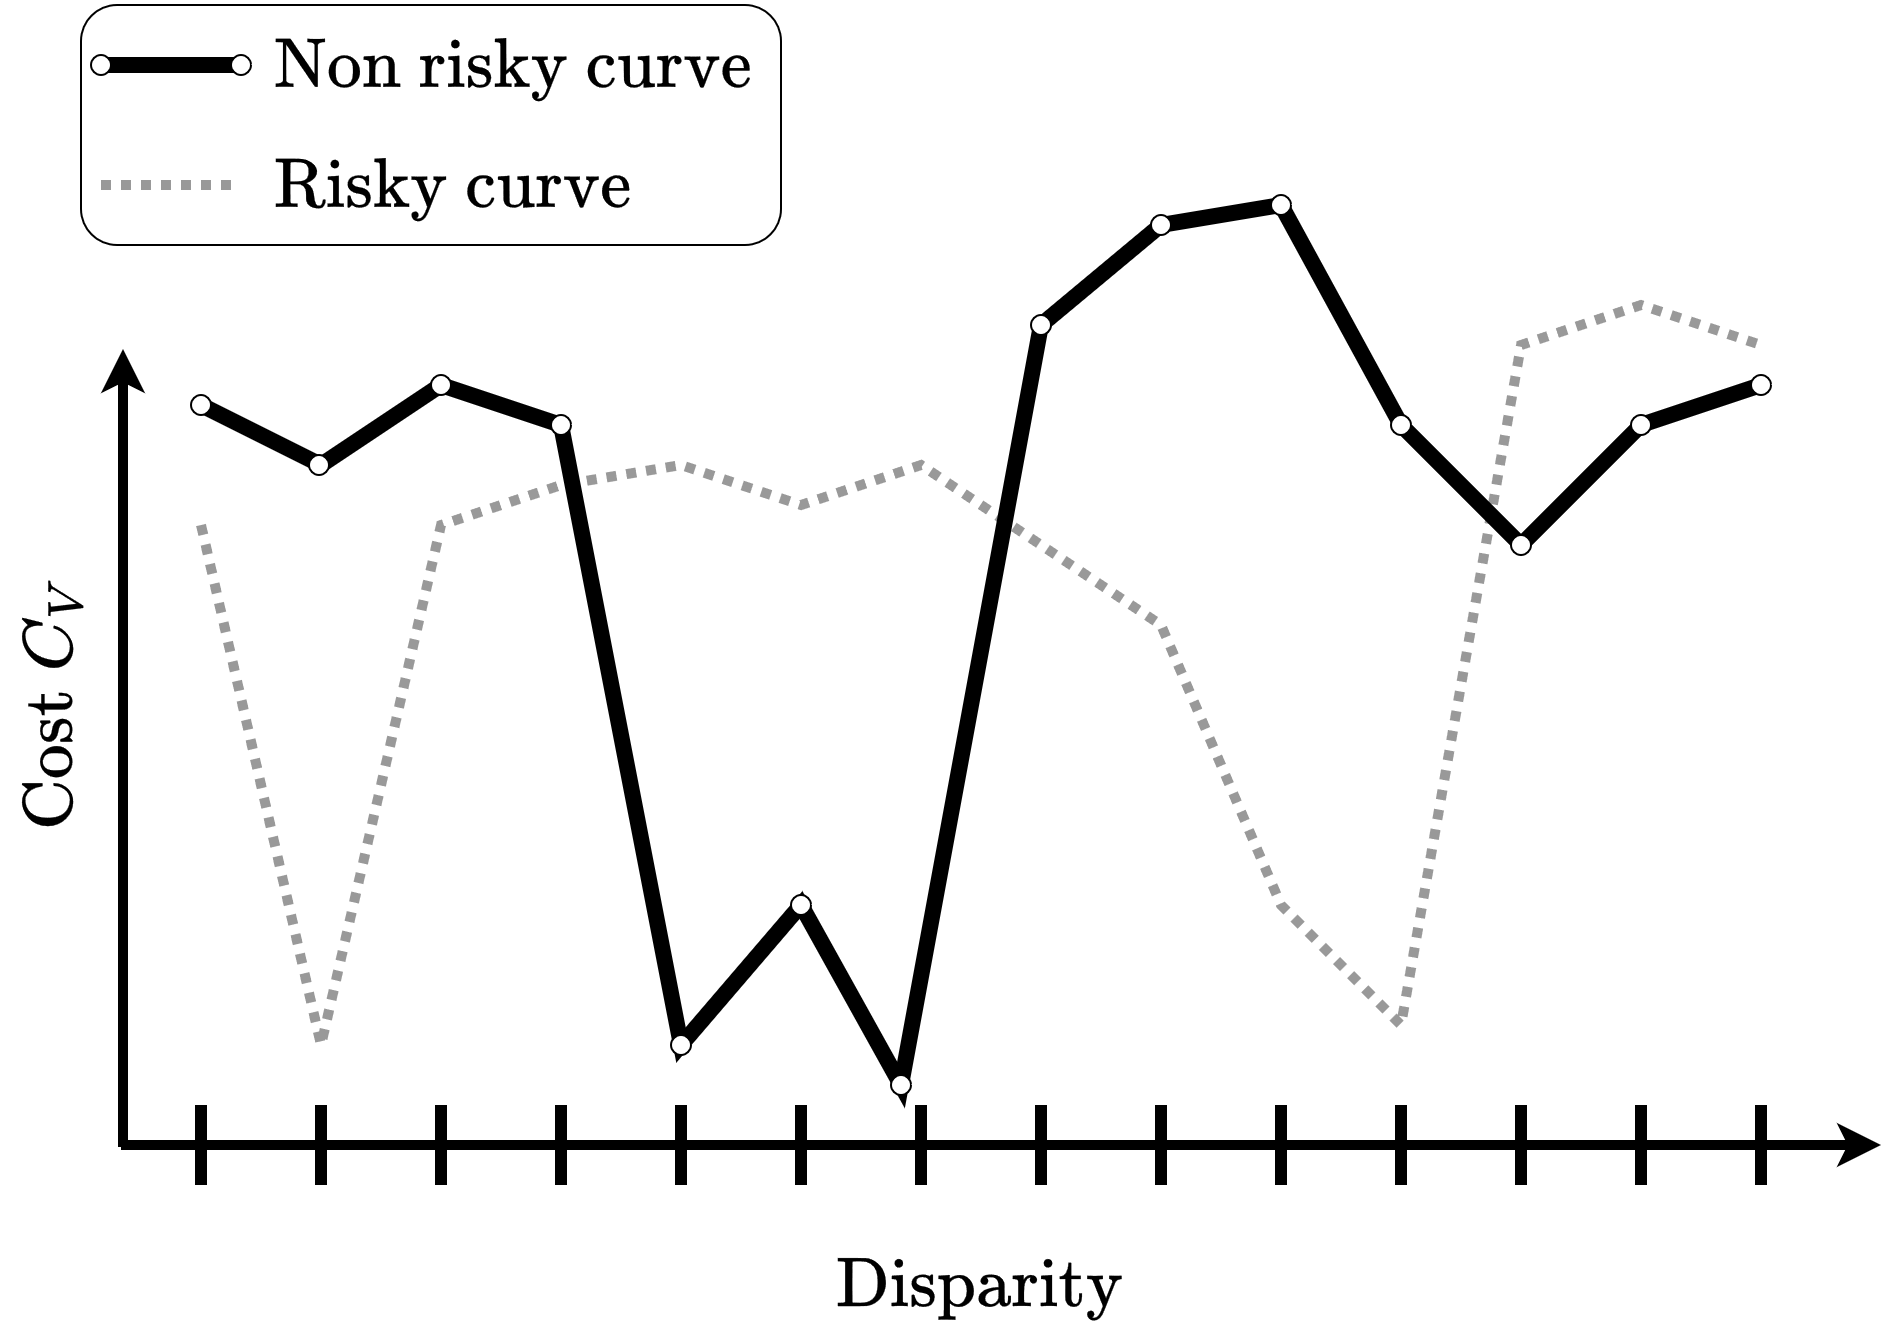
\includegraphics[width=\linewidth]{Images/Chap_1/Risk.png}
        \caption{}
        \label{fig:risk}
    \end{subfigure}\hfill
    \caption{Cost curves with different levels of ambiguity \ref{fig:ambgiuity} and risk \ref{fig:risk}}
    \label{fig:ambiguity_risk}
\end{figure}

The first confidence measure is a confidence measure called \textit{confidence from ambiguity} \cite{sarrazin_ambiguity_2021}. This method is based on the cost volume and quantifies how easy or hard it is to single out the correct disparity in a cost curve. \Cref{fig:ambgiuity} presents two curves: one that is ambiguous and one that is not\commanue{Alors tu as une phrase qui reprend cette info en la complétant donc cette phrase est en trop.}. To compute it, we first start by constructing what is called an \textit{ambiguity curve}. We do that by counting how many disparities have a cost close within a threshold $\eta$ to the minimal cost, for increasing values of $\eta$. \Cref{fig:ambgiuity} presents two cost curves, one which is not ambiguous as there is a single well defined minimum, and an ambiguous cost curve which presents multiple values that are close to the minimum. Formally we need to define for a pixel $(row, ~col)$ the set of all disparities whose cost is within a range $\eta$ of the minimal cost, and then define the ambiguity curve as the cardinal of this set:
\begin{align}
    &\mathcal{D}_\eta = \{d ~|~ C_V(row,~col,~d) \leqslant \min_\delta C_V(row, ~col, ~\delta) + \eta\}\\
    &Amb(row, ~col, ~\eta) = \#\mathcal{D}_\eta
\end{align}
where $\#$ is the cardinal of a set. Evaluating $Amb$ for different $\eta$ gives the ambiguity curve. \Cref{fig:integral_ambiguity_1} presents a cost curve with different values of $\eta$. \Cref{fig:integral_ambiguity_2} presents the resulting ambiguity curve. On those two figures we can see for instance that for $\eta_3$ there are $6$ disparities whose cost is lower than $\min_\delta C_V(row, ~col, ~\delta) + \eta_3$. For non-ambiguous cost curves, $Amb$ will increase only for high values of $\eta$. On the contrary, for ambiguous curves, $Amb$ will be high for small values of $\eta$. To obtain a scalar value from $Amb$, we compute the area under its curve, normalized by the range of $\eta$:
\begin{equation}
    \mathrm{AUC}_{Amb}(row, ~col) = \frac{1}{\max\eta-\min\eta}\int_\eta Amb(row,~col,~\eta)d\eta
\end{equation}
However, this results on low values for confident (non-ambiguous) cost curves, and high values for less confident (ambiguous) curves. The confidence from ambiguity $c_{Amb}$ is thus obtained by normalizing and reverting the integral:
\begin{equation}\label{eq:confidence_from_ambiguity}
    c_{Amb}(row, ~col) = \frac{\max \mathrm{AUC}_{Amb}- \mathrm{AUC}_{Amb}(row, ~col)}{\max \mathrm{AUC}_{Amb} -\min \mathrm{AUC}_{Amb}}
\end{equation}
This way, values of $c_{Amb}$ near $0$ indicate that we are not confident in the predicted disparity. Reversely, values of $c_{Amb}$ near $1$ indicate that we are confident in the predicted disparity.

\begin{figure}
    \centering
    \begin{subfigure}[t]{0.6\linewidth}
        \centering
        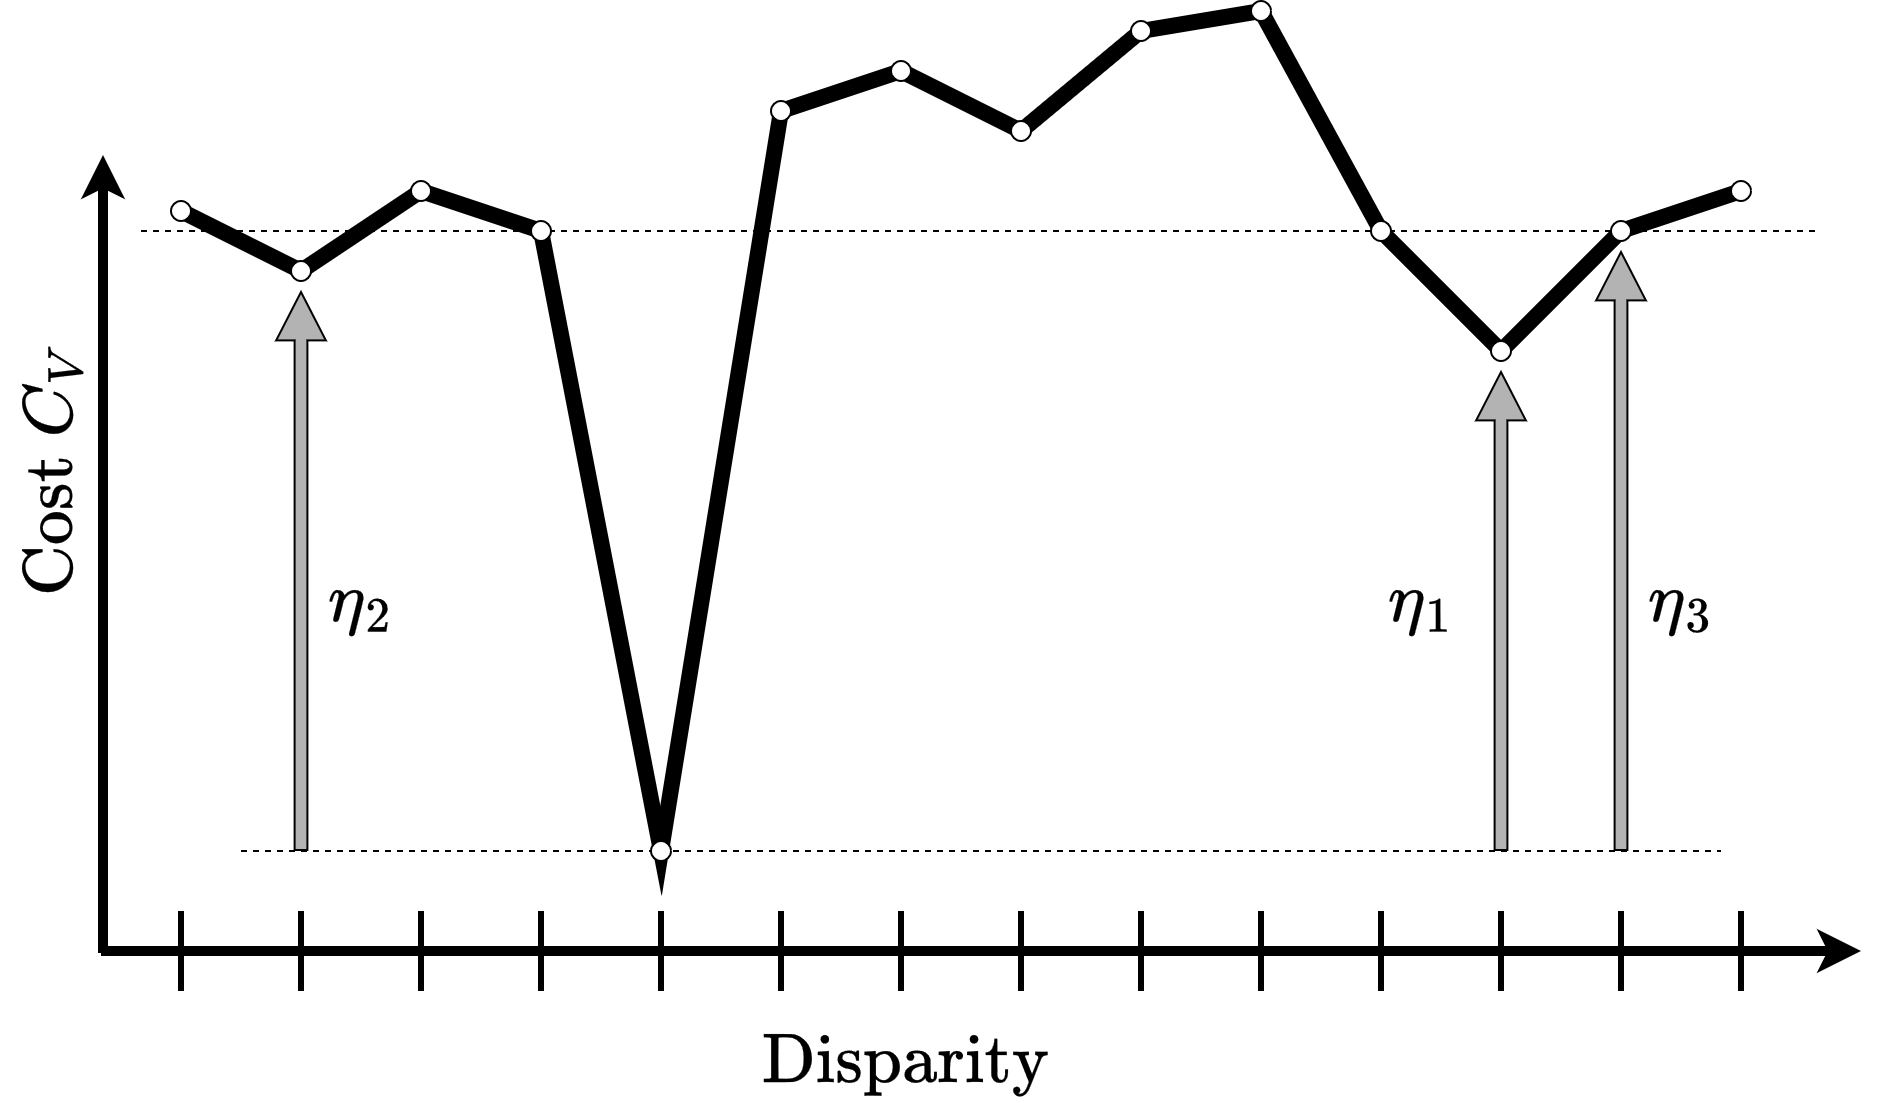
\includegraphics[width=\linewidth]{Images/Chap_1/Integral_Ambiguity_1.png}
        \caption{Cost curve with different values of $\eta$. Horizontal dotted lines indicates the range of costs between $\min_\delta C_V(row, ~col, ~\delta)$ and $\min_\delta C_V(row, ~col, ~\delta)+\eta_3$}
        \label{fig:integral_ambiguity_1}
    \end{subfigure}\hfill
    \begin{subfigure}[t]{0.4\linewidth}
        \centering
        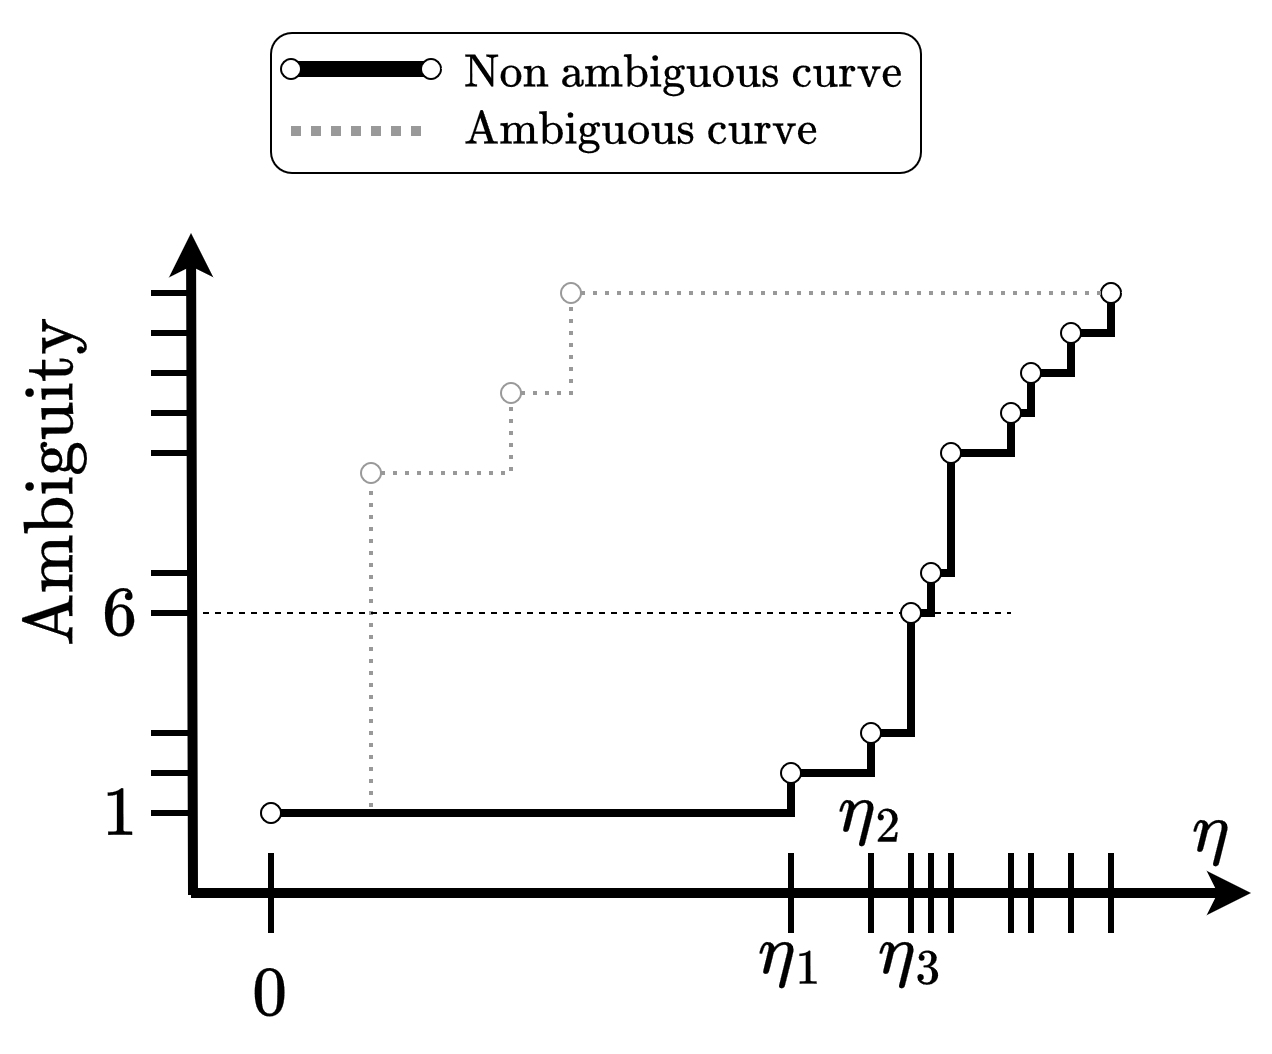
\includegraphics[width=\linewidth]{Images/Chap_1/Integral_Ambiguity_2.png}
        \caption{Associated ambiguity curve in full line. Ambiguous curve in gray dotted line}
        \label{fig:integral_ambiguity_2}
    \end{subfigure}\hfill
    \caption{Illustration of the computation of the ambiguity curve.}
    \label{fig:integral_ambiguity}
\end{figure}

The second confidence measure that we consider is named \textit{confidence from risk}. It is designed to measure if the magnitude of a potential error is high or low. After all, if we predict a wrong disparity while the correct disparity is right next to our prediction, the impact on the final result will be smaller than if the true disparity is at the other side of the disparity range. Keeping this in mind, we apply the same methodology as for the ambiguity. We consider the set $\mathcal{D}_\eta$ of all disparities whose cost is less than $\eta$ away from the minimal cost, and define the risk as the gap between extrema of this set:
\begin{equation}
    R(row, ~col, ~\eta) = \max_{\mathcal{D}_\eta}d - \min_{\mathcal{D}_\eta}d
\end{equation}
\Cref{fig:integral_risk_1} presents a cost curve with different values of $\eta$ and their associated risk $R$. \Cref{fig:integral_risk_2} presents the resulting risk for all $\eta$. For non-risky cost curves, $R$ will increase only for high values of $\eta$. On the contrary, for risky curves, $R$ will be high for small values of $\eta$. To obtain a single scalar, we compute the area under the risk curve, normalized by the range of $\eta$:
\begin{equation}
    \mathrm{AUC}_R = \frac{1}{\max\eta-\min\eta}\int_\eta R(row,~col,~\eta)d\eta
\end{equation}
$\mathrm{AUC}_R$ is thus expressed in number of disparities. Contrary to the confidence from ambiguity, the risk is kept as such with its current unity. 

\begin{remark}
     The risk measures the magnitude of the potential error, but not its probability. It is therefore possible to have a very risky cost curve, but which is not ambiguous at all. In other words, it means that the probability of an error occurring can be very low, but if it somehow happened, then the magnitude of this error would also be very low. The risk is thus a confidence measure that need to be completed by a measure such as ambiguity. On it own, it has less meaning than other measures.
     
    \begin{comment}
        As detailed in \Cref{sec:co3d}, one of the requirements of the CO3D mission is to produce a performance map associated with the output DSM, expressed in meters. In order to produce such a performance map, one of the leads explored at CNES was to combine the confidence from ambiguity and the risk. This is done by weighting the risk with $1-c_{Amb}$, so as to reduce the risk of confident pixels. The result, expressed in number of disparities, can itself be converted into meters using the disparity to altitude ratio $d_{alt}$ computed along epipolar grids (see \Cref{sec:epipolar_geometry}). Finally, internal studies using real data have concluded that a good candidate for a performance criterion was:
        \begin{equation}
            perf(row, ~col) = \min(1, ~\frac{1-c_{amb}(row,~col)}{\tau_{amb}})\cdot \mathrm{AUC}_R(row,~col) \cdot d_{alt}
        \end{equation}
        where $\tau_{amb}$ is a threshold usually set to $0.4$. In plain words, if the confidence from ambiguity drops below $1-\tau_{amb}$, then we do not use the ambiguity weighting and the performance equals $\mathrm{AUC}_R \cdot d_{alt}$. This performance criterion thus provide a confidence measure expressed in meters, associated to a 3D point, which can then be rasterized alongside the DSM to produce the desired performance map. We will use it as a comparison for our method in \Cref{chap:epistemic_uncertainty}.
    \end{comment}
\end{remark}

\todoroman{Dire qu'il y a eu des tentatives internes pour allier risk et amb pour faire une carte de perf. Nos travaux s'inscrivent dans cette continuité pour proposer une autre méthode. Il est envisagé de peut être l'utiliser dans la chaine CO3D.}

\begin{figure}
    \centering
    \begin{subfigure}[t]{0.6\linewidth}
        \centering
        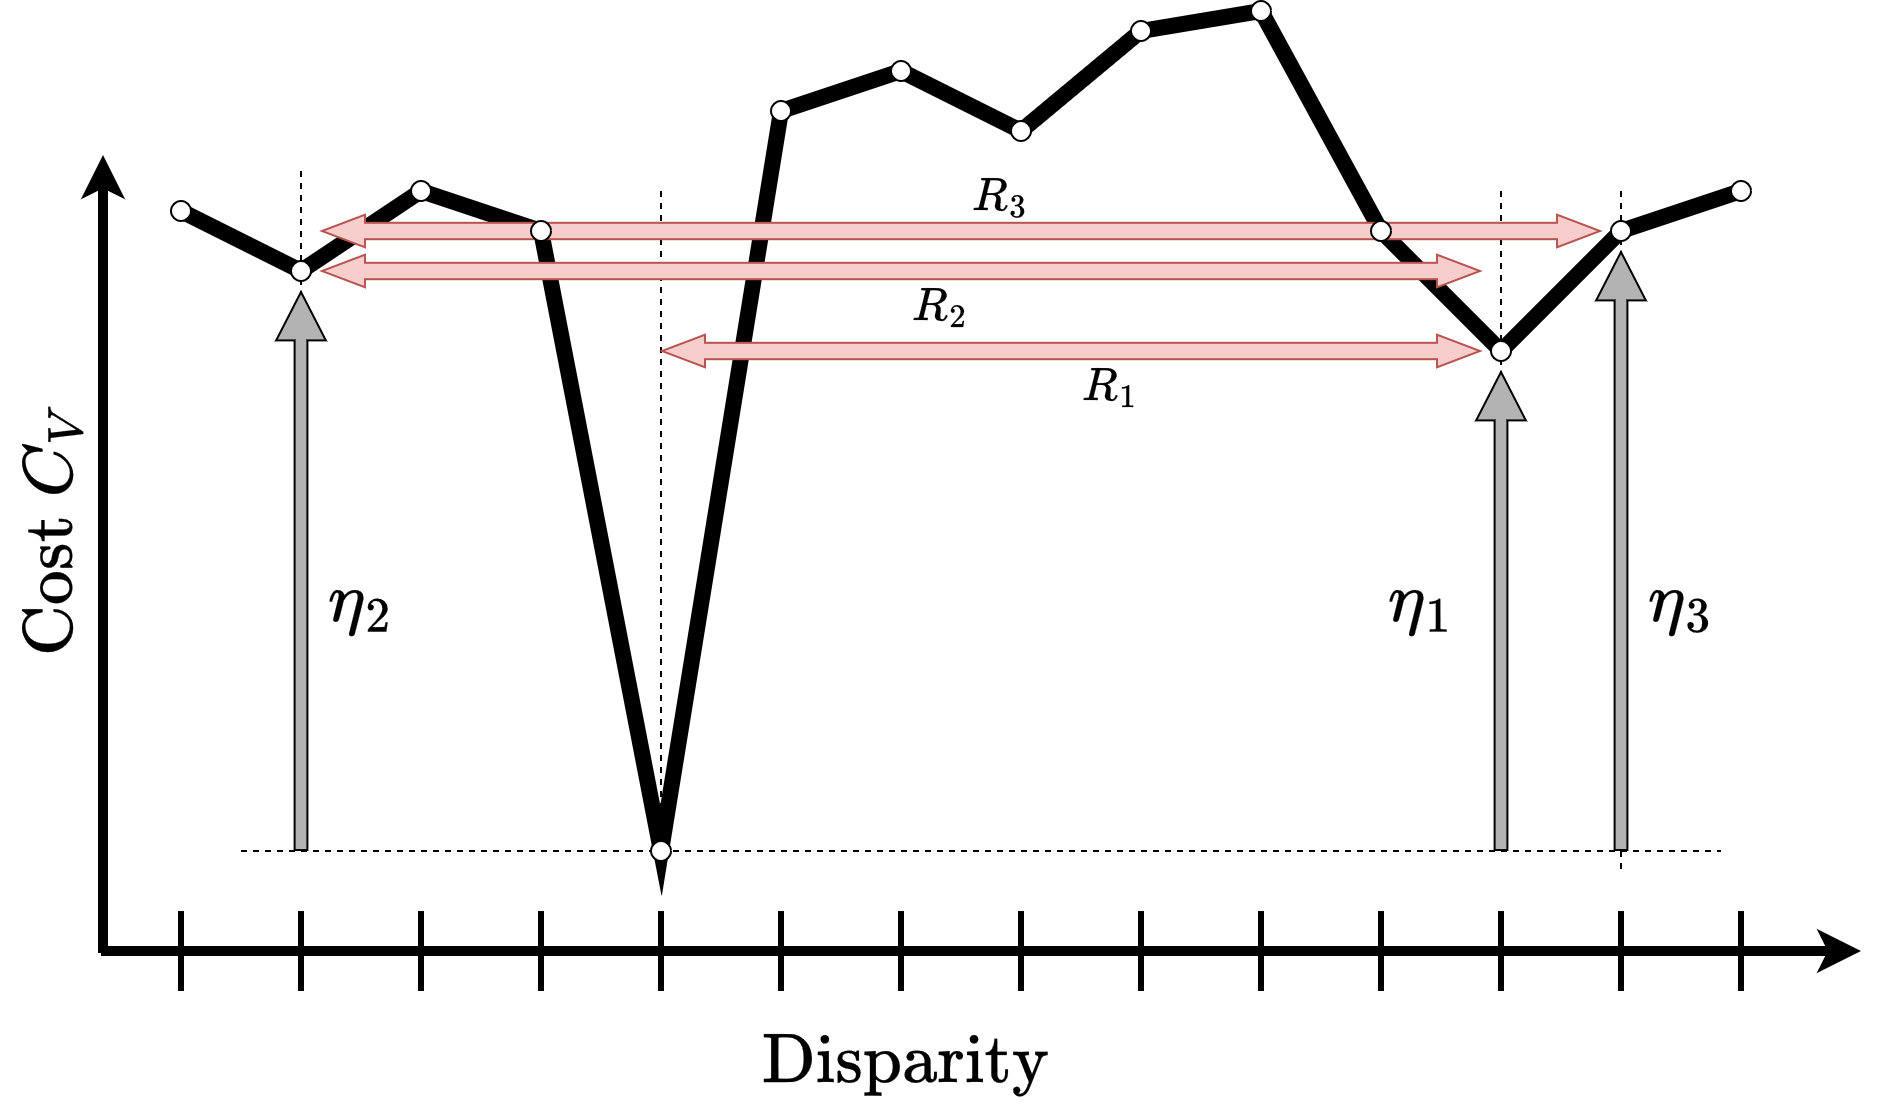
\includegraphics[width=\linewidth]{Images/Chap_1/Integral_Risk_1.png}
        \caption{Cost curve with different values of $\eta$ and risk}
        \label{fig:integral_risk_1}
    \end{subfigure}\hfill
    \begin{subfigure}[t]{0.4\linewidth}
        \centering
        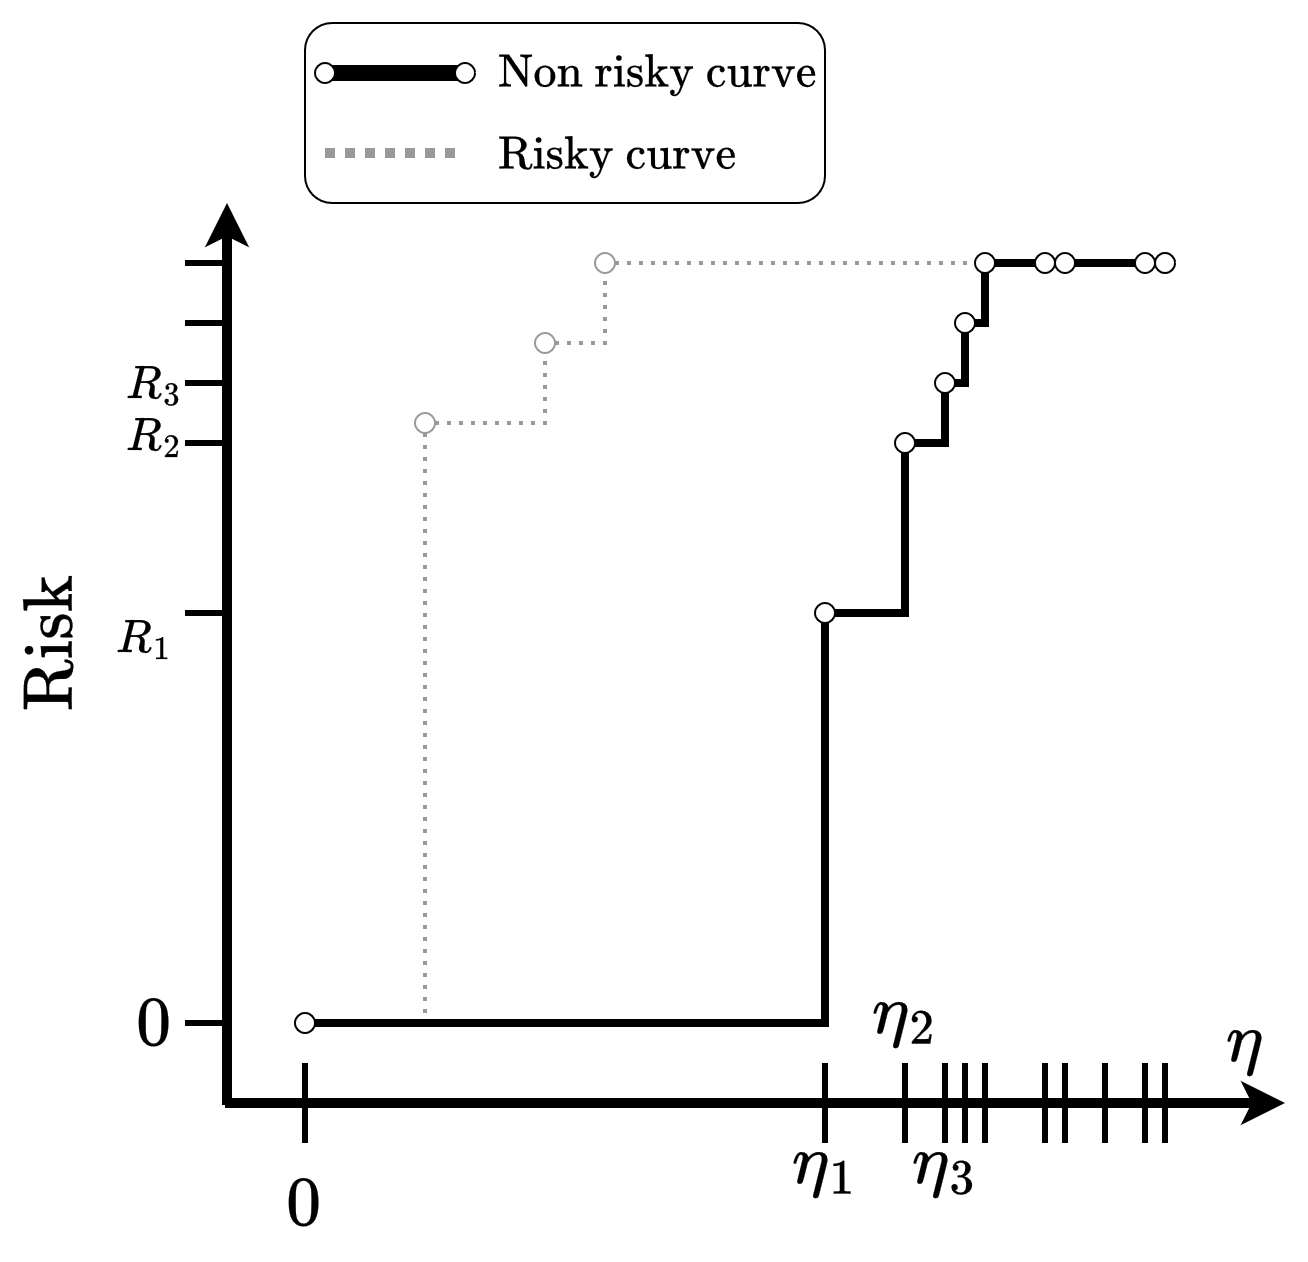
\includegraphics[width=\linewidth]{Images/Chap_1/Integral_Risk_2.png}
        \caption{Associated risk curve in full line. Risky curve in gray dotted line}
        \label{fig:integral_risk_2}
    \end{subfigure}\hfill
    \caption{Illustration of the computation of the risk curve.}
    \label{fig:integral_risk}
\end{figure}

\commanue{pas de conclusion ? en même temps tu reste constant avec tes principes}
\pagebreak
\blankpage
